\documentclass{article}

% --- NeurIPS 2026 style ---
\usepackage{neurips_2026}

% --- Packages ---
\usepackage[utf8]{inputenc}
\usepackage[T1]{fontenc}
\usepackage{amsmath, amssymb, amsthm}
\usepackage{mathtools}
\usepackage{booktabs}
\usepackage{graphicx}
\usepackage{algorithm}
\usepackage{algorithmic}
\usepackage[colorlinks=true,citecolor=blue,linkcolor=blue,urlcolor=blue]{hyperref}
\usepackage{cleveref}
\usepackage{xcolor}
\usepackage{microtype}
\usepackage{enumitem}
\usepackage{wrapfig}
\usepackage{tikz}
\usetikzlibrary{patterns,arrows.meta,decorations.pathreplacing}

% --- Theorem Environments ---
\newtheorem{definition}{Definition}
\newtheorem{theorem}{Theorem}
\newtheorem{lemma}{Lemma}
\newtheorem{proposition}{Proposition}
\newtheorem{corollary}{Corollary}
\newtheorem{assumption}{Assumption}
\newtheorem{remark}{Remark}
\newtheorem{example}{Example}

% --- Custom Commands ---
\newcommand{\thetavec}{\boldsymbol{\theta}}
\newcommand{\R}{\mathbb{R}}
\newcommand{\E}{\mathbb{E}}
\newcommand{\Prob}{\mathbb{P}}
\newcommand{\ind}{\mathbf{1}}
\newcommand{\cS}{\mathcal{S}}
\newcommand{\cA}{\mathcal{A}}
\newcommand{\cM}{\mathcal{M}}
\newcommand{\cT}{\mathcal{T}}
\newcommand{\cB}{\mathcal{B}}
\newcommand{\cN}{\mathcal{N}}
\newcommand{\Sviol}{\mathcal{S}_{\mathrm{viol}}}
\newcommand{\piord}{\pi_{\mathrm{ord}}}
\newcommand{\Rmax}{R_{\max}}
\newcommand{\Vmax}{V_{\max}}
\DeclareMathOperator*{\argmax}{arg\,max}
\DeclareMathOperator*{\argmin}{arg\,min}
\DeclareMathOperator{\sign}{sign}
\DeclareMathOperator{\Lip}{Lip}
\DeclareMathOperator{\Var}{Var}

% ============================================================
\title{Ordinal MDP: Zero-Shot Policy Transfer \\ via Ordinal Consistency}

\author{Anonymous Author(s)}

\begin{document}
\maketitle

% ============================================================
\begin{abstract}
A reinforcement learning policy trained at Earth gravity ($9.8$\,m/s$^2$) is asked to act in a low-gravity environment ($5$\,m/s$^2$). Does it still act optimally? The standard answer tracks how far the Q-\emph{values} drifted, but a greedy policy depends only on the \emph{ordering} of actions, not their magnitudes: it transfers without retraining exactly when the rank of the best action at each state survives the shift. We capture this by the \emph{action-gap distribution} $F_\kappa$ of the source environment, which records how decisively each state prefers its top action over the runner-up. Our central result, the Violation Growth Theorem, bounds the fraction of states where the policy fails by $F_\kappa(2 L_Q \|\Delta\theta\|)$: only states whose action gap is smaller than the perturbation can flip. This bound is tight to factor $1$ for every $\gamma \in [0,1)$, recovers a quadratic-in-$\|\Delta\theta\|$ degradation law for continuous actions, yields a stability radius for safe deployment, and admits a source-side diagnostic that combines policy-agreement statistics with a finite-difference upper bound on $L_Q$ (using a user-supplied curvature constant and critic tolerance, valid on the source support; no target rewards or rollouts are used). Across discrete and continuous control benchmarks, $F_\kappa$ measured from source data alone correctly predicts which environments transfer gracefully and identifies the regime in which the quadratic refinement holds. $F_\kappa$ is a structural fingerprint of an environment: measured from source data alone, it indicates when zero-shot transfer is likely to remain reliable under physics shifts.
\end{abstract}

% ============================================================
\section{Introduction}
\label{sec:intro}
% ============================================================

Transferring reinforcement learning (RL) policies across environments with different physical dynamics (the \emph{sim-to-real} problem) is a central challenge in robot learning~\citep{zhao2020sim, muratore2022robot}. Standard approaches learn \emph{cardinal} value information: domain randomization averages over parameter distributions~\citep{tobin2017domain, peng2018sim}, system identification estimates parameters online~\citep{ljung1998system, yu2017preparing}, and meta-learning adapts value functions to new tasks~\citep{finn2017model, rakelly2019efficient}. All require either target-domain interaction, reward access, or both.

We ask a more basic question:
\begin{quote}
\emph{Under what conditions is ordinal information (the ordering of actions by Q-value) sufficient for zero-shot policy transfer?}
\end{quote}

If the ordering of actions is preserved when gravity changes from $9.8$ to $5$\,m/s$^2$, then a policy learned under $9.8$ is already optimal under $5$ without adaptation, reward access, or target interaction. This observation motivates the \emph{Ordinal MDP} framework (Figure~\ref{fig:framework}).

\textbf{Why ordinal?} Action orderings are more robust than values: as parameters shift, all Q-values drift, but the relative ranking of actions persists wherever the perturbation is small relative to the action gap (Theorem~\ref{thm:violation-growth}). The action-gap CDF $F_\kappa$ measured on the source side then determines, before any target interaction, what fraction of states can possibly flip under a given $\|\Delta\theta\|$. Multi-source aggregation inherits scale-invariance: majority voting over orderings is immune to magnitude differences, while Q-value averaging is not (\S\ref{sec:exp-baselines}, \S\ref{sec:exp-neural}).

\begin{figure}[t]
\centering
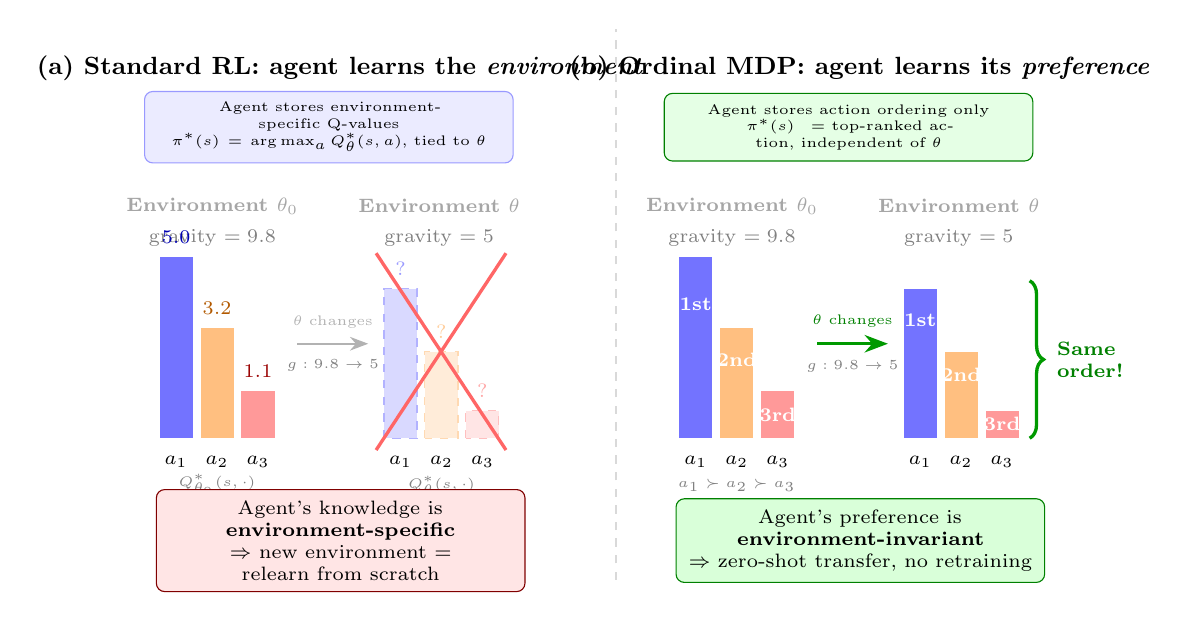
\begin{tikzpicture}[every node/.style={font=\footnotesize}]

  % ========== Panel (a): Standard MDP — agent learns the environment ==========
  \begin{scope}[shift={(-5.8,0)}]
    \node[font=\small\bfseries] at (2.3,5.3) {(a) Standard RL: agent learns the \emph{environment}};

    % What agent stores
    \node[fill=blue!8, draw=blue!40, rounded corners=3pt, inner sep=4pt, font=\tiny, text width=4.4cm, align=center] at (2.15,4.55) {Agent stores environment-specific Q-values\\$\pi^*(s) = \argmax_a Q^*_\theta(s,a)$, tied to $\theta$};

    % --- Source environment ---
    \node[font=\scriptsize\bfseries, gray!70] at (0.67,3.55) {Environment $\theta_0$};
    \node[font=\scriptsize, gray] at (0.67,3.15) {gravity $= 9.8$};
    % Q-bars with numerical values
    \fill[blue!55] (0,0.6) rectangle (0.42,2.9);
    \fill[orange!50] (0.52,0.6) rectangle (0.94,2.0);
    \fill[red!40] (1.04,0.6) rectangle (1.46,1.2);
    \node[font=\scriptsize] at (0.21,0.3) {$a_1$};
    \node[font=\scriptsize] at (0.73,0.3) {$a_2$};
    \node[font=\scriptsize] at (1.25,0.3) {$a_3$};
    % Values prominently displayed
    \node[font=\scriptsize\bfseries, blue!70!black] at (0.21,3.15) {$5.0$};
    \node[font=\scriptsize\bfseries, orange!70!black] at (0.73,2.25) {$3.2$};
    \node[font=\scriptsize\bfseries, red!60!black] at (1.25,1.45) {$1.1$};
    \node[font=\tiny, gray] at (0.73,0.0) {$Q^*_{\theta_0}(s,\cdot)$};

    % --- Arrow: environment changes ---
    \draw[-{Stealth}, thick, gray!60] (1.75,1.8) -- (2.65,1.8)
      node[midway, above=2pt, font=\tiny] {$\theta$ changes}
      node[midway, below=2pt, font=\tiny, gray] {$g: 9.8 \to 5$};

    % --- New environment ---
    \node[font=\scriptsize\bfseries, gray!70] at (3.55,3.55) {Environment $\theta$};
    \node[font=\scriptsize, gray] at (3.55,3.15) {gravity $= 5$};
    % Ghost bars (unknown values)
    \fill[blue!15, draw=blue!30, dashed] (2.85,0.6) rectangle (3.27,2.5);
    \fill[orange!15, draw=orange!30, dashed] (3.37,0.6) rectangle (3.79,1.7);
    \fill[red!10, draw=red!25, dashed] (3.89,0.6) rectangle (4.31,0.95);
    \node[font=\scriptsize] at (3.06,0.3) {$a_1$};
    \node[font=\scriptsize] at (3.58,0.3) {$a_2$};
    \node[font=\scriptsize] at (4.10,0.3) {$a_3$};
    % Question marks
    \node[font=\scriptsize\bfseries, blue!40] at (3.06,2.75) {$?$};
    \node[font=\scriptsize\bfseries, orange!40] at (3.58,1.95) {$?$};
    \node[font=\scriptsize\bfseries, red!35] at (4.10,1.2) {$?$};
    \node[font=\tiny, gray] at (3.58,0.0) {$Q^*_{\theta}(s,\cdot)$};

    % Red X overlay
    \draw[red!60, very thick] (2.75,0.45) -- (4.4,2.95);
    \draw[red!60, very thick] (2.75,2.95) -- (4.4,0.45);

    % Result box
    \node[fill=red!10, draw=red!50!black, rounded corners=3pt, inner sep=4pt, font=\scriptsize, text width=4.4cm, align=center] at (2.3,-0.7) {Agent's knowledge is \textbf{environment-specific}\\$\Rightarrow$ new environment $=$ relearn from scratch};
  \end{scope}

  % ========== Vertical divider ==========
  \draw[gray!30, thick, dashed] (0.0,-1.2) -- (0.0,5.8);

  % ========== Panel (b): Ordinal MDP — agent learns its own preference ==========
  \begin{scope}[shift={(0.8,0)}]
    \node[font=\small\bfseries] at (2.3,5.3) {(b) Ordinal MDP: agent learns its \emph{preference}};

    % What agent stores
    \node[fill=green!10, draw=green!50!black, rounded corners=3pt, inner sep=4pt, font=\tiny, text width=4.4cm, align=center] at (2.15,4.55) {Agent stores action ordering only\\$\pi^*(s) = $ top-ranked action, independent of $\theta$};

    % --- Source environment ---
    \node[font=\scriptsize\bfseries, gray!70] at (0.67,3.55) {Environment $\theta_0$};
    \node[font=\scriptsize, gray] at (0.67,3.15) {gravity $= 9.8$};
    % Same Q-bars
    \fill[blue!55] (0,0.6) rectangle (0.42,2.9);
    \fill[orange!50] (0.52,0.6) rectangle (0.94,2.0);
    \fill[red!40] (1.04,0.6) rectangle (1.46,1.2);
    \node[font=\scriptsize] at (0.21,0.3) {$a_1$};
    \node[font=\scriptsize] at (0.73,0.3) {$a_2$};
    \node[font=\scriptsize] at (1.25,0.3) {$a_3$};
    % Ordinal labels instead of values
    \node[font=\scriptsize\bfseries, white] at (0.21,2.3) {1st};
    \node[font=\scriptsize\bfseries, white] at (0.73,1.6) {2nd};
    \node[font=\scriptsize\bfseries, white] at (1.25,0.9) {3rd};
    \node[font=\tiny, gray] at (0.73,0.0) {$a_1 \succ a_2 \succ a_3$};

    % --- Arrow: environment changes ---
    \draw[-{Stealth}, very thick, green!60!black] (1.75,1.8) -- (2.65,1.8)
      node[midway, above=2pt, font=\tiny, green!50!black] {$\theta$ changes}
      node[midway, below=2pt, font=\tiny, gray] {$g: 9.8 \to 5$};

    % --- New environment ---
    \node[font=\scriptsize\bfseries, gray!70] at (3.55,3.55) {Environment $\theta$};
    \node[font=\scriptsize, gray] at (3.55,3.15) {gravity $= 5$};
    % Bars with different heights but SAME ordering
    \fill[blue!55] (2.85,0.6) rectangle (3.27,2.5);
    \fill[orange!50] (3.37,0.6) rectangle (3.79,1.7);
    \fill[red!40] (3.89,0.6) rectangle (4.31,0.95);
    \node[font=\scriptsize] at (3.06,0.3) {$a_1$};
    \node[font=\scriptsize] at (3.58,0.3) {$a_2$};
    \node[font=\scriptsize] at (4.10,0.3) {$a_3$};
    % Same ordinal labels
    \node[font=\scriptsize\bfseries, white] at (3.06,2.1) {1st};
    \node[font=\scriptsize\bfseries, white] at (3.58,1.4) {2nd};
    \node[font=\scriptsize\bfseries, white] at (4.10,0.78) {3rd};

    % Green brace
    \draw[decorate, decoration={brace, amplitude=5pt}, very thick, green!60!black]
      (4.45,2.6) -- (4.45,0.6) node[midway, right=6pt, font=\scriptsize\bfseries, green!50!black, text width=1.2cm, align=left] {Same\\order!};

    % Result box
    \node[fill=green!15, draw=green!50!black, rounded corners=3pt, inner sep=4pt, font=\scriptsize, text width=4.4cm, align=center] at (2.3,-0.7) {Agent's preference is \textbf{environment-invariant}\\$\Rightarrow$ zero-shot transfer, no retraining};
  \end{scope}

\end{tikzpicture}
\caption{\textbf{Standard RL vs.\ Ordinal MDP} under a gravity shift ($9.8 \to 5$\,m/s$^2$). \textbf{(a)}~Standard RL stores Q-values that become invalid when $\theta$ shifts. \textbf{(b)}~An Ordinal MDP stores only the action ordering ($a_1 \succ a_2 \succ a_3$), preserved within the stability radius $\rho = \kappa_{\min}/(2L_Q)$ (Theorems~\ref{thm:transfer-gap},~\ref{thm:stability-radius}), enabling zero-shot transfer.}
\label{fig:framework}
\end{figure}

\textbf{Contributions.} Our central result is that the action gap distribution $F_\kappa$ characterizes transfer robustness:
\begin{enumerate}[leftmargin=*,itemsep=1pt,topsep=2pt]
\item \textbf{$F_\kappa$ as the right object: matching tightness for all $\gamma$ plus informational necessity.} Individual ingredients used along the way (Performance Difference Lemma, Lipschitz $Q$ sensitivity, action gap as a per-MDP scalar) are classical; our contribution is the action-gap \emph{distribution} $F_\kappa$ as the population-level object that governs transfer. The violation growth theorem (Theorem~\ref{thm:violation-growth}) shows the violation fraction scales as $F_\kappa(2L_Q\|\Delta\theta\|)$. Matching constructions (Propositions~\ref{prop:tight-growth},~\ref{prop:tight-growth-gamma}) saturate the bound to factor $1$ for every $\gamma \in [0,1)$ on a worst-case Lipschitz family (the standard meaning of upper-bound tightness; non-adversarial families like the chain MDP of Appendix~\ref{app:gamma-tightness} have substantially looser actual rates). The full distribution is moreover \emph{informationally necessary}: any predictor depending only on $\kappa_{\min}$ and the median of $F_\kappa$ leaves the violation rate undetermined up to an arbitrary multiplicative factor $K$ (Proposition~\ref{prop:fkappa-necessity}). The transfer gap decomposition (Theorem~\ref{thm:transfer-gap}) is a direct restriction of PDL to $\Sviol$ and serves as the enabling lemma rather than an independent contribution.
\item \textbf{Corollaries of $F_\kappa$.} The $F_\kappa$ framework yields: (a)~an ordinal stability radius $\rho = \kappa/(2L_Q)$ via Bellman sensitivity (\S\ref{sec:stability}); (b)~quadratic degradation $O(\|\Delta\theta\|^2)$ for continuous actions via implicit differentiation of the Bellman equation (\S\ref{sec:continuous}); (c)~a within-support source-agreement certificate for data-driven OC verification with no target-reward access (\S\ref{sec:model-free}); and (d)~a finite-difference upper bound on $L_Q$ from the same source ensemble (Proposition~\ref{prop:lq-estimator}), replacing direct $L_Q$ knowledge by the milder smoothness $H_Q$ and critic-error $\varepsilon_Q$ inputs.
\item \textbf{Experiments} spanning tabular MDPs, LQR, DQN, Gymnasium, and MuJoCo with SAC ($d=3$ parameter variation, 3 seeds): tabular and discrete-control predictions hold quantitatively; on MuJoCo, $F_\kappa$ correctly ranks all three environments by transfer fragility, and multi-seed transfer-gap slopes stay strictly below the quadratic upper bound on Hopper ($\approx 1.17$) and HalfCheetah ($\approx 1.20$), as Theorem~\ref{thm:continuous-bound-main} predicts (it is an upper, not exact, slope), while Ant ($\approx 2.52$) exceeds it. The strong-concavity diagnostic in Appendix~\ref{app:hessian-diag} localizes the deviation to environments and gravities where Assumption~\ref{asm:local-sc} empirically collapses (\S\ref{sec:experiments}).
\end{enumerate}

% ============================================================
\section{Preliminaries}
\label{sec:prelim}
% ============================================================

\begin{definition}[Parameterized MDP Family]
\label{def:param-mdp}
A \emph{parameterized MDP family} is $\cM = \{M_\theta\}_{\theta \in \Theta}$ with $\Theta \subseteq \R^d$, where each $M_\theta = (\cS, \cA, P_\theta, R_\theta, \gamma)$ shares state space $\cS$, action space $\cA$, and discount $\gamma \in [0,1)$, with parameter-dependent transition $P_\theta : \cS \times \cA \to \Delta(\cS)$ and reward $R_\theta : \cS \times \cA \to [0, \Rmax]$.
\end{definition}

We allow $\cA$ to be finite (\S\ref{sec:transfer-bound}--\S\ref{sec:sample-complexity-discrete}) or a compact convex subset of $\R^m$ (\S\ref{sec:continuous}). The optimal Q-function, value, and policy are $Q^*_\theta$, $V^*_\theta$, $\pi^*_\theta = \argmax_a Q^*_\theta(\cdot, a)$, with $\Vmax = \Rmax/(1-\gamma)$. The \emph{Q-gap} is $G_\theta(s,a,a') \coloneqq Q^*_\theta(s,a) - Q^*_\theta(s,a')$ and the \emph{discounted visitation} is $d^\pi_{\theta,\rho}(s) \coloneqq (1-\gamma)\sum_{t=0}^{\infty}\gamma^t \Prob^{\pi,\theta}(s_t = s \mid s_0 \sim \rho)$.

\begin{definition}[Ordinal Consistency]
\label{def:oc}
$\cM$ is \emph{ordinally consistent} (OC) at state $s$ if for all $\theta_1, \theta_2 \in \Theta$ and $a, a' \in \cA$:
$G_{\theta_1}(s,a,a') > 0 \implies G_{\theta_2}(s,a,a') > 0$.
$\cM$ is \emph{globally OC} if this holds at every $s \in \cS$.
\end{definition}

\begin{definition}[Violation Set]
\label{def:viol}
$\Sviol(\theta_0,\theta) \coloneqq \{s \in \cS : \pi^*_{\theta_0}(s) \neq \pi^*_{\theta}(s)\}$. The per-state suboptimality gap $\Delta_{\theta}(s) \coloneqq V^*_{\theta}(s) - Q^*_{\theta}(s, \pi^*_{\theta_0}(s)) \geq 0$ vanishes outside $\Sviol$.
\end{definition}

% ============================================================
\section{Transfer Gap via Violation States}
\label{sec:transfer-bound}
% ============================================================

The central question of policy transfer is: \emph{how much performance do we lose by deploying a source-optimal policy in a target environment?} The classical Simulation Lemma~\citep{kearns2002near} bounds this loss using worst-case distributional distance. We decompose it over the states where the source policy's action ordering is actually violated.

\begin{theorem}[Transfer Gap Decomposition]
\label{thm:transfer-gap}
Let $\pi_0 = \pi^*_{\theta_0}$ be deployed in $M_{\theta}$. For any initial distribution $\rho$:
\begin{equation}
\label{eq:transfer-exact}
\boxed{V^*_{\theta}(\rho) - V^{\pi_0}_{\theta}(\rho) = \frac{1}{1-\gamma}\sum_{s \in \Sviol(\theta_0,\theta)} d^{\pi_0}_{\theta,\rho}(s)\;\Delta_{\theta}(s).}
\end{equation}
\end{theorem}

\begin{proof}
The Performance Difference Lemma~\citep{kakade2002approximately} gives:
$V^{\pi'}_\theta(\rho) - V^{\pi}_\theta(\rho) = \frac{1}{1-\gamma}\sum_{s} d^{\pi}_{\theta,\rho}(s)\,A^{\pi'}_\theta(s, \pi(s))$.
Setting $\pi = \pi_0$, $\pi' = \pi^*_{\theta}$ in $M_{\theta}$, and noting $A^*_{\theta}(s, \pi_0(s)) = -\Delta_{\theta}(s)$ with $\Delta_{\theta}(s) = 0$ outside $\Sviol$, we obtain~\eqref{eq:transfer-exact}.
\end{proof}

\begin{remark}[Relation to Simulation Lemma]
\label{rem:sim-lemma}
Restricting to $\Sviol$, weighting by actual visitation, and using per-state cost $\Delta_\theta(s) \ll \Vmax$ make~\eqref{eq:transfer-exact} structurally tighter than the Simulation Lemma; its key value is enabling the violation growth analysis below.
\end{remark}

\subsection{Violation Growth and Graceful Degradation}
\label{sec:violation-growth}

Theorem~\ref{thm:transfer-gap} decomposes the transfer gap over $\Sviol$, but how does $|\Sviol|$ grow as the parameter shifts? The answer depends on the \emph{distribution of action gaps} across states.

\begin{definition}[Action Gap and its CDF]
\label{def:gap-cdf}
The per-state action gap is $\kappa(s, \theta_0) = \min_{a \neq \pi^*_{\theta_0}(s)} [Q^*_{\theta_0}(s, \pi^*_{\theta_0}(s)) - Q^*_{\theta_0}(s, a)]$, and its global minimum is $\kappa(\theta_0) = \min_s \kappa(s, \theta_0)$. The action gap CDF is $F_\kappa(x) = |\{s : \kappa(s, \theta_0) \leq x\}| / |\cS|$.
\end{definition}

\begin{theorem}[Violation Growth Rate]
\label{thm:violation-growth}
Under Assumption~\ref{asm:lipschitz}:
\begin{enumerate}[leftmargin=*,itemsep=1pt]
\item $|\Sviol(\theta_0, \theta)| / |\cS| \leq F_\kappa(2L_Q\|\theta - \theta_0\|)$.
\item The transfer gap satisfies:
\begin{equation}
\label{eq:graceful}
V^*_\theta(\rho) - V^{\pi_0}_\theta(\rho) \leq \frac{\Vmax}{1-\gamma} \cdot F_\kappa(2L_Q\|\theta - \theta_0\|).
\end{equation}
\end{enumerate}
\end{theorem}

\begin{proof}
(i) If $\kappa(s, \theta_0) > 2L_Q\|\Delta\theta\|$, then by Lemma~\ref{lem:q-lipschitz}, every Q-gap changes by at most $2L_Q\|\Delta\theta\|$, so the ordering at $s$ is preserved and $s \notin \Sviol$. By contrapositive, $s \in \Sviol \Rightarrow \kappa(s, \theta_0) \leq 2L_Q\|\Delta\theta\|$. (ii) Apply Theorem~\ref{thm:transfer-gap} with $\Delta_\theta(s) \leq \Vmax$ and $d^{\pi_0}_{\theta,\rho}(s) \leq 1/(1-\gamma)$. When $F_\kappa$ is Lipschitz near the origin ($F_\kappa(x) \leq cx$), the gap is thus linear in $\|\Delta\theta\|$; a tighter continuous-action bound combining this with Theorem~\ref{thm:quadratic-subopt} is given in Appendix~\ref{app:tight-violation}.
\end{proof}

Unlike the Simulation Lemma's uniform $|\cS|\Vmax$ scaling, \eqref{eq:graceful} exploits $F_\kappa$'s shape (linearity in $\|\Delta\theta\|$ requires $F_\kappa(x) \leq cx$ near zero, generic under smooth parameterizations) and can be much tighter (\S\ref{sec:exp-transfer-gap}). The full distribution is moreover necessary, not stylistic: any predictor depending only on $\kappa_{\min}$ and the median of $F_\kappa$ leaves the violation rate undetermined up to an arbitrary multiplicative factor (Proposition~\ref{prop:fkappa-necessity}, with $2.6$--$22\times$ MSE separation in Table~\ref{tab:shape-vs-median}). Appendix~\ref{app:tight-growth} constructs a Lipschitz MDP saturating the bound to factor $1$ for every $\gamma \in [0,1)$ (Propositions~\ref{prop:tight-growth} and~\ref{prop:tight-growth-gamma}); the $(1-\gamma)^{-1}$ factor inside $L_Q$ is information-theoretically necessary for any reward-Lipschitz-based bound. The empirical $5.2\times$ looseness on the chain MDP of Appendix~\ref{app:gamma-tightness} reflects that the chain family is not worst-case (Remark~\ref{rem:gamma-positive-tightness}).

% ============================================================
\section{Ordinal Stability Radius}
\label{sec:stability}
% ============================================================

When is ordinal consistency guaranteed? We derive computable certificates.

\subsection{Conservative Radius via Lipschitz Bounds}

\begin{assumption}[Lipschitz MDP Family]
\label{asm:lipschitz}
$|R_{\theta_1}(s,a) - R_{\theta_2}(s,a)| \leq L_R\|\theta_1 - \theta_2\|$ and $|P_{\theta_1}(s'|s,a) - P_{\theta_2}(s'|s,a)| \leq L_P\|\theta_1 - \theta_2\|$ for all $(s,a,s')$.
\end{assumption}

Under Assumption~\ref{asm:lipschitz}, the optimal Q-function is Lipschitz in $\theta$ with constant $L_Q = (L_R + \gamma|\cS|L_P\Vmax)/(1-\gamma)$ (Lemma~\ref{lem:q-lipschitz}, Appendix~\ref{app:proofs}). This controls how fast Q-gaps can close under perturbation.

\begin{theorem}[Conservative Stability Radius]
\label{thm:stability-radius}
Under Assumption~\ref{asm:lipschitz}: $\rho_{\mathrm{cons}}(\theta_0) \coloneqq \frac{\kappa(\theta_0)}{2L_Q}$ satisfies $\|\theta - \theta_0\| < \rho_{\mathrm{cons}}(\theta_0) \implies \Sviol(\theta_0, \theta) = \emptyset$.
\end{theorem}
\begin{proof}
For $s \in \cS$ and $a \neq \pi^*_{\theta_0}(s)$: $G_{\theta_0}(s,\pi^*_{\theta_0}(s),a) \geq \kappa(\theta_0)$. Since $|G_\theta - G_{\theta_0}| \leq 2L_Q\|\theta - \theta_0\|$ by Lemma~\ref{lem:q-lipschitz}, if $\|\theta-\theta_0\| < \kappa(\theta_0)/(2L_Q)$, then $G_\theta(s,\pi^*_{\theta_0}(s),a) > 0$.
\end{proof}

\subsection{Tight Radius via Bellman Sensitivity}

The conservative radius uses the global Lipschitz constant $2L_Q$. Under $C^1$ smoothness of $R_\theta, P_\theta$ in $\theta$ (Assumption~\ref{asm:smooth}, Appendix~\ref{app:proofs}), differentiating the Bellman optimality equation yields a closed-form Q-value sensitivity $\mathbf{s}_\theta$ (Proposition~\ref{prop:sensitivity}), and the Q-gap sensitivity is $\sigma_\theta(s,a,a') = s_\theta(s,a) - s_\theta(s,a')$. Intuitively, $|\sigma_\theta|$ captures the \emph{actual} rate at which a given Q-gap changes, which can be much smaller than the worst-case $2L_Q$ because the latter bounds every gap simultaneously along every path. Replacing $2L_Q$ with the per-gap rate $\sup_\theta|\sigma_\theta|$ gives $\rho_{\mathrm{tight}}(\theta_0) = \min_{s,\, a \neq a'} |G_{\theta_0}(s,a,a')|/\sup_{\theta \in \Theta_{\mathrm{reg}}}|\sigma_\theta(s,a,a')| \geq \rho_{\mathrm{cons}}(\theta_0)$ (Theorem~\ref{thm:tight-stability}, Appendix~\ref{app:proofs}).

\textbf{Empirical tightening.} On an 8-state chain (Appendix~\ref{app:exp-stability}), $\rho_{\mathrm{tight}} = 0.367$ vs.\ $\rho_{\mathrm{cons}} = 0.018$---a $20.8\times$ improvement; both are valid lower bounds on the true OC region. For neural MuJoCo policies, direct $\rho_{\mathrm{tight}}$ requires Bellman sensitivity under function approximation, so we use the empirical strong-concavity margin (Appendix~\ref{app:hessian-diag}) as a proxy.

% ============================================================
\section{Continuous Action Spaces}
\label{sec:continuous}
% ============================================================

We extend to $\cA \subset \R^m$ (compact, convex), studying the optimal action map $a^*_\theta(s) = \argmax_{a \in \cA} Q^*_\theta(s,a)$. In this setting, exact ordinal consistency (identical optima) is measure-zero; the relevant question is \emph{how fast does the transfer gap grow?}

\begin{assumption}[Local Strong Concavity]
\label{asm:local-sc}
There exist $\mu, L_{aa} > 0$ such that $-L_{aa}\mathbf{I} \preceq \nabla^2_{aa}Q^*_\theta(s,a) \preceq -\mu\mathbf{I}$ for all $a$ near $a^*_\theta(s)$, uniformly in $s$ and $\theta$.
\end{assumption}
\begin{assumption}[Basin Dominance]
\label{asm:basin-dom}
The global optimum dominates: $Q^*_\theta(s, a^*_\theta(s)) - \sup_{a \notin \cB_\theta(s)} Q^*_\theta(s, a) \geq \delta_{\mathrm{basin}} > 0$, where $\cB_\theta(s)$ is the strong concavity basin.
\end{assumption}
\begin{assumption}[Interior Optimum and Joint Smoothness]
\label{asm:interior}
$a^*_\theta(s) \in \mathrm{int}(\cA)$ for all $\theta, s$, and $Q^*_\theta(s,a)$ is $C^2$ in $a$ and $C^1$ in $\theta$.
\end{assumption}

Two ingredients drive the continuous bound: (i) a \emph{quadratic suboptimality} bound $\Delta_\theta(s) \leq \tfrac{L_{aa}}{2}\|a^*_\theta(s) - a^*_{\theta_0}(s)\|^2$ from local strong concavity; (ii) an \emph{action displacement} bound $\|a^*_\theta(s) - a^*_{\theta_0}(s)\| \leq \Lambda(s)\|\theta - \theta_0\|/\mu$ from the implicit function theorem applied to $\nabla_a Q^*_\theta(s, a^*_\theta(s)) = 0$, where $\Lambda(s) = \sup_\theta\|\nabla^2_{a\theta}Q^*_\theta\|_{\mathrm{op}}$. Chaining them and summing via Theorem~\ref{thm:transfer-gap} yields:

\begin{theorem}[Continuous Transfer Bound, informal]
\label{thm:continuous-bound-main}
Under Assumptions~\ref{asm:local-sc}--\ref{asm:interior}, for $\|\theta-\theta_0\|$ sufficiently small,
\[
V^*_\theta(\rho) - V^{\pi_0}_\theta(\rho) \;\leq\; \frac{L_{aa}\Lambda_{\max}^2}{2\mu^2(1-\gamma)}\,\|\theta-\theta_0\|^2, \qquad \Lambda_{\max} = \max_s \Lambda(s).
\]
\end{theorem}

This is qualitatively different from the $O(\|\Delta\theta\|)$ Simulation Lemma bound and is a direct consequence of the smooth optimality landscape. Full statement and proof: Theorem~\ref{thm:continuous-bound} in Appendix~\ref{app:proofs}.

% ============================================================
\section{Sample Complexity}
\label{sec:sample-complexity}
% ============================================================

Given $K$ source environments $\theta_1, \ldots, \theta_K \overset{\text{i.i.d.}}{\sim} \mu$, how many suffice to recover the correct ordinal policy?

\subsection{Discrete Actions}
\label{sec:sample-complexity-discrete}

\begin{definition}[Population Ordinal Margin]
\label{def:pop-margin}
$\kappa_{\min} = \min_{s,\,a \neq a'}|\Prob_{\theta \sim \mu}[G_\theta(s,a,a')>0] - 1/2| > 0$.
\end{definition}

This quantifies how decisively the population ``votes'' for one action over another. When $\kappa_{\min} > 0$, majority voting over $K$ i.i.d.\ source policies recovers the population-optimal ordering at every state with probability $\geq 1 - \delta$ once $K = \Theta(\kappa_{\min}^{-2}\log(|\cS||\cA|^2/\delta))$ (Theorem~\ref{thm:sample-complexity}, Appendix~\ref{app:proofs}), via a Hoeffding bound on each of $|\cS|\binom{|\cA|}{2}$ pairwise comparisons---the classical Condorcet jury theorem~\citep{young1988condorcet} applied to action orderings. Noisy Q-estimates $\|\hat{Q}_{\theta_k} - Q^*_{\theta_k}\|_\infty \leq \epsilon_Q$ preserve all ordinal comparisons provided the minimum nonzero Q-gap $g_{\min} > 2\epsilon_Q$ (Corollary~\ref{cor:noisy-q}, Appendix~\ref{app:proofs}).

\subsection{Continuous Actions}
\label{sec:sample-continuous}

For continuous actions, the mean-action policy $\bar{a}(s) = \frac{1}{K}\sum_{k=1}^K a^*_{\theta_k}(s)$ converges at the standard $O(1/K)$ rate with an irreducible $\Var_\mu[a^*_\theta(s)]$ bias from the source distribution not centering on the target (Theorem~\ref{thm:continuous-sample}, Appendix~\ref{app:proofs}). This bias vanishes asymptotically only if the target is drawn from $\mu$, which is one reason our certificate in \S\ref{sec:model-free} restricts guarantees to within $\operatorname{supp}(\mu)$.

\subsection{Source-Agreement Certificates}
\label{sec:model-free}

The stability radius and violation growth (Theorems~\ref{thm:stability-radius},~\ref{thm:violation-growth}) require model access to compute $\kappa(s)$ and $L_Q$. We show $\kappa_{\min}$ can instead be lower-bounded \emph{from source policy agreement alone}, certifying OC at $\theta \in \operatorname{supp}(\mu)$; extension outside the support (the typical sim-to-real regime) further relies on $L_Q$ (Corollary~\ref{cor:model-free-transfer}, Algorithm~\ref{alg:ordinal-transfer}).

\begin{proposition}[Source-Agreement Certificate]
\label{prop:model-free}
Given $K$ source policies $\pi^*_{\theta_k}$ with $\theta_k \overset{\text{i.i.d.}}{\sim} \mu$, let $\hat{\eta} = \min_{s,\,a \neq a'} |\hat{p}(s, a, a') - \tfrac{1}{2}|$ where $\hat{p}(s, a, a') = \frac{1}{K}\sum_k \ind[G_{\theta_k}(s, a, a') > 0]$. With probability $\geq 1 - \delta$,
\begin{equation}
\label{eq:model-free-margin}
\kappa_{\min} \;\geq\; \hat{\kappa} \;:=\; \hat{\eta} - \sqrt{\tfrac{\ln(2|\cS|\binom{|\cA|}{2}/\delta)}{2K}}.
\end{equation}
If $\hat{\kappa} > 0$, the source distribution $\mu$ satisfies OC with positive margin, and the stability radius is at least $\hat{\rho} = \hat{\kappa}/(2L_Q)$.
\end{proposition}

\begin{proof}
Hoeffding on each of $|\cS|\binom{|\cA|}{2}$ i.i.d.\ Bernoulli pairs with a union bound gives $|\hat{p} - \Prob_\mu[G_\theta > 0]| \leq \sqrt{\ln(2|\cS|\binom{|\cA|}{2}/\delta)/(2K)}$ simultaneously; subtracting $1/2$ and taking $\min$ yields~\eqref{eq:model-free-margin}.
\end{proof}

\textbf{Protocol.} Train $K$ policies under diverse $\theta_k\sim\mu$, count action agreements, obtain $\hat\kappa$ and the empirical radius $\hat\rho=\hat\kappa/(2L_Q)$. Algorithm~\ref{alg:ordinal-transfer} (Appendix~\ref{app:algorithm}) then deploys in three regimes: \textbf{certified} ($\theta\in\operatorname{supp}(\mu)$, $\|\theta-\theta_0\|<\hat\rho$ $\Rightarrow$ gap $=0$); \textbf{extrapolated} (out of support, contingent on $L_Q$ along the path); \textbf{bounded} (outside the radius, gap $\leq \tfrac{2\Vmax}{1-\gamma}\int_0^{2L_Q\|\theta-\theta_0\|}F_\kappa(x)\,dx$). The $L_Q$ dependence is itself estimable from the same source ensemble (Proposition~\ref{prop:lq-estimator} below); the union-bound sharpening to $\log\mathcal{N}_\varepsilon(\cS)$ is in Appendix~\ref{app:covering-number}.

\begin{proposition}[Source-Side Certified $L_Q$ Estimator]
\label{prop:lq-estimator}
Let $\Theta = [\theta_{\min}, \theta_{\max}] \subset \R$ and assume $Q^*_\theta(s,a)$ is twice continuously differentiable in $\theta$ with $\sup_{s,a,\theta} |\partial^2_\theta Q^*_\theta(s,a)| \leq H_Q$. Let $\theta_{\min} = \theta_1 < \cdots < \theta_K = \theta_{\max}$ span $\Theta$ with gaps $h_k = \theta_{k+1} - \theta_k$, and let $\hat Q_{\theta_k}$ be source-side critic estimates with $\sup_{s,a} |\hat Q_{\theta_k}(s,a) - Q^*_{\theta_k}(s,a)| \leq \varepsilon_Q$. Then
\begin{equation}
\label{eq:lq-cert}
L_Q \;\leq\; \hat L_Q^{\mathrm{cert}} \;:=\; \max_{s,a}\,\max_{1 \leq k < K} \!\left[\,\frac{|\hat Q_{\theta_{k+1}}(s,a) - \hat Q_{\theta_k}(s,a)| + 2\varepsilon_Q}{h_k} + H_Q\, h_k\,\right].
\end{equation}
Substituting $\hat L_Q^{\mathrm{cert}}$ for $L_Q$ in Proposition~\ref{prop:model-free} preserves the OC margin guarantee while replacing direct knowledge of $L_Q$ by the (typically milder) inputs $H_Q$ and $\varepsilon_Q$. The proof is in Appendix~\ref{app:lq-estimator-proof}.
\end{proposition}

% ============================================================
% ============================================================
\section{Experiments}
\label{sec:experiments}
% ============================================================

We validate the Ordinal MDP framework through three main experiments: transfer gap decomposition on tabular MDPs, baseline comparisons, and neural policies (DQN on Gymnasium and SAC on MuJoCo). Additional experiments---ordinal stability radius, LQR quadratic degradation (\S\ref{sec:exp-lqr}), control-environment transfer (Wind Grid + Pendulum), sample complexity, and a 4-joint robot surrogate---are deferred to Appendix~\ref{app:additional-exp} for space; multi-dimensional ($d=3$) parameter transfer is in Appendix~\ref{app:exp-multidim}. Code is available in the supplementary material.

% ────────────────────────────────────────────────────────────
\subsection{Transfer Gap Decomposition (Theorem~\ref{thm:transfer-gap})}
\label{sec:exp-transfer-gap}
% ────────────────────────────────────────────────────────────

\paragraph{Setup.} $5 \times 5$ grid-world MDP family parameterized by $\theta \in [0,1]$ controlling wind strength and step cost. Source policy $\pi^*_{\theta_0}$ at $\theta_0 = 0$, deployed across 50 target parameters.

\paragraph{Results.} Our decomposition matches the true gap exactly while the Simulation Lemma overestimates by $3{,}600$--$123{,}700\times$ (Figure~\ref{fig:transfer-gap}(a,b))---it sums over all $|\cS|{=}25$ states (vs.\ $|\Sviol|{\leq}2$), uses worst-case $\Vmax$, and ignores visitation; when $\Sviol{=}\emptyset$ our bound is zero while the Simulation Lemma exceeds $200$. Figure~\ref{fig:transfer-gap}(d) validates Theorem~\ref{thm:violation-growth}: $F_\kappa(2L_Q\|\Delta\theta\|)$ upper-bounds the actual violation fraction at all parameters. Appendix~\ref{app:perstate} confirms the mechanism: states violate in order of increasing $\kappa(s)$.

\begin{figure}[t]
\centering
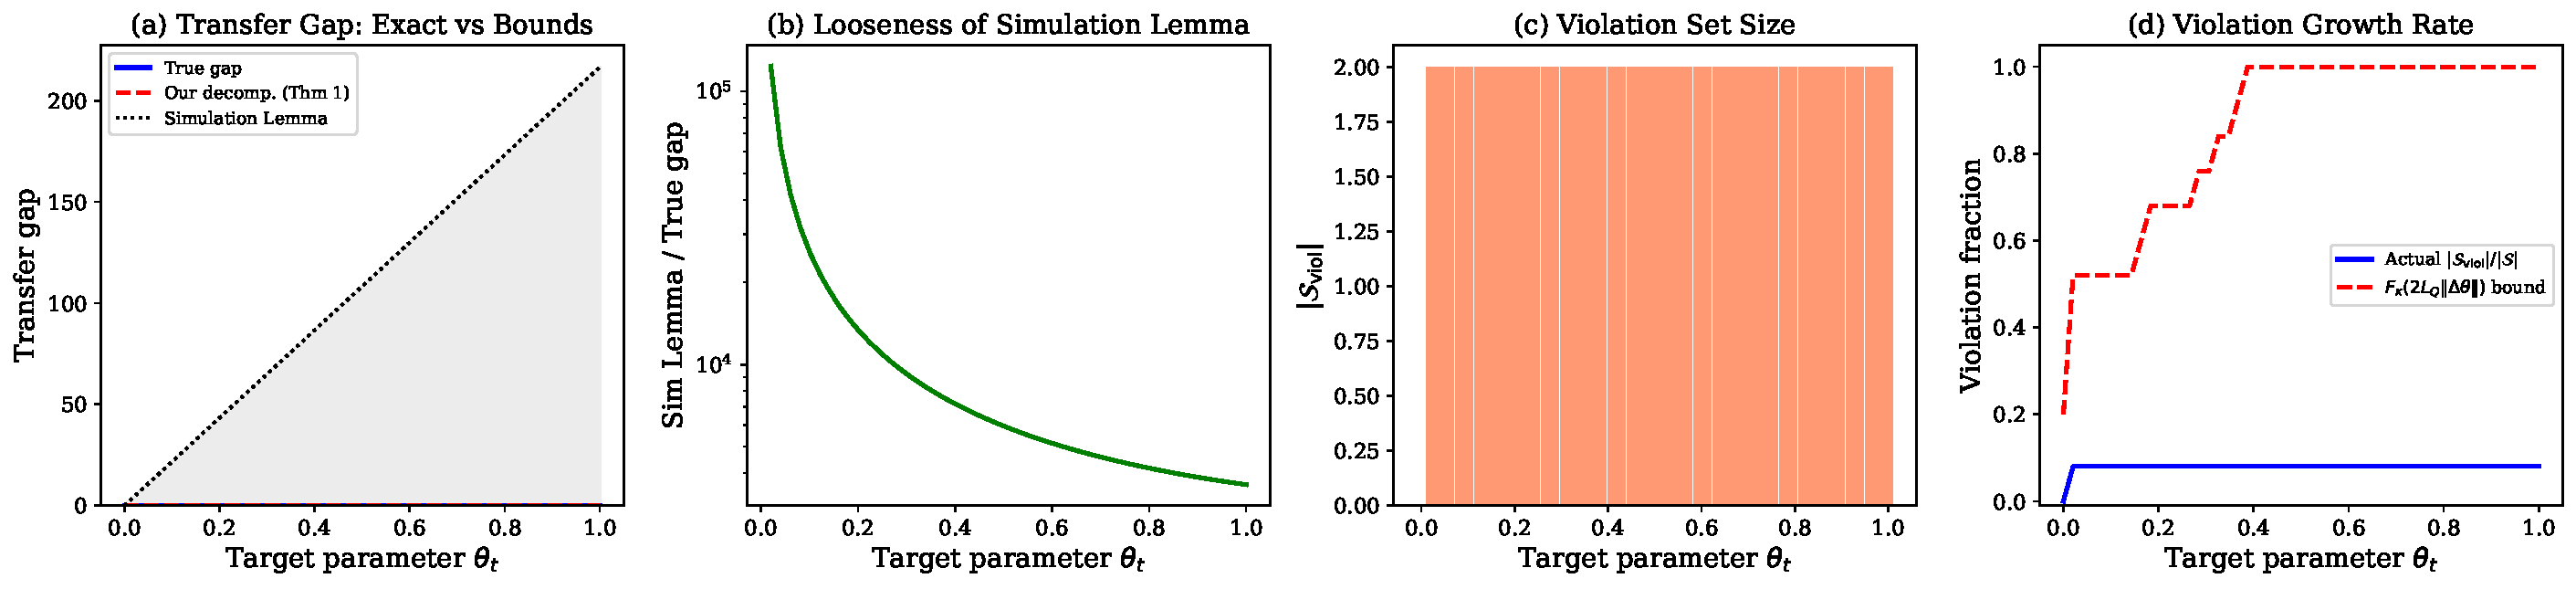
\includegraphics[width=\textwidth]{figures/exp1_transfer_gap.pdf}
\caption{Transfer gap decomposition. (a) Our decomposition (Thm.~\ref{thm:transfer-gap}) matches the true gap; the Simulation Lemma is orders of magnitude loose. (b) Looseness ratio (log scale). (c) $|\Sviol| \leq 2$ out of 25 states. (d) Violation growth: $F_\kappa(2L_Q\|\Delta\theta\|)$ upper-bounds the actual violation fraction (Thm.~\ref{thm:violation-growth}).}
\label{fig:transfer-gap}
\end{figure}

% ────────────────────────────────────────────────────────────
% §7.2 Quadratic Degradation in LQR moved to Appendix~\ref{app:exp-lqr}
% ────────────────────────────────────────────────────────────

% ────────────────────────────────────────────────────────────
\subsection{Comparison with Transfer Baselines}
\label{sec:exp-baselines}
% ────────────────────────────────────────────────────────────

\paragraph{Setup.} $10 \times 10$ grid with two competing goals, wind, and ice ($\theta \in \R^3$). Sources have \emph{heterogeneous reward scales}: each source's Q-values are multiplied by a random factor in $[1/r, r]$ for scale range $r$, simulating environments with different reward magnitudes. We compare: Ordinal (majority-vote, $K=30$), Domain Randomization (solve mean MDP with scaled rewards), Q-Averaging (mean of scaled Q-values), Robust (maximin), and Single Source.

\paragraph{Results.} The ordinal policy is scale-invariant by construction: its transfer gap stays at $4.6$ across all scale ranges $r$ (Figure~\ref{fig:baselines}(c)), while Q-Averaging degrades from $8.2$ to $12.9$ and DR from $4.9$ to $5.8$ as $r$ grows from $1$ to $50\times$. Overall, Ordinal (avg.\ gap $17.4$) beats Q-Averaging ($25.2$), Robust ($39.2$), Single Source ($19.8$) and matches DR ($17.1$); ordinal beats DR in regions far from the source center (Figure~\ref{fig:baselines}(f)).

\begin{figure}[t]
\centering
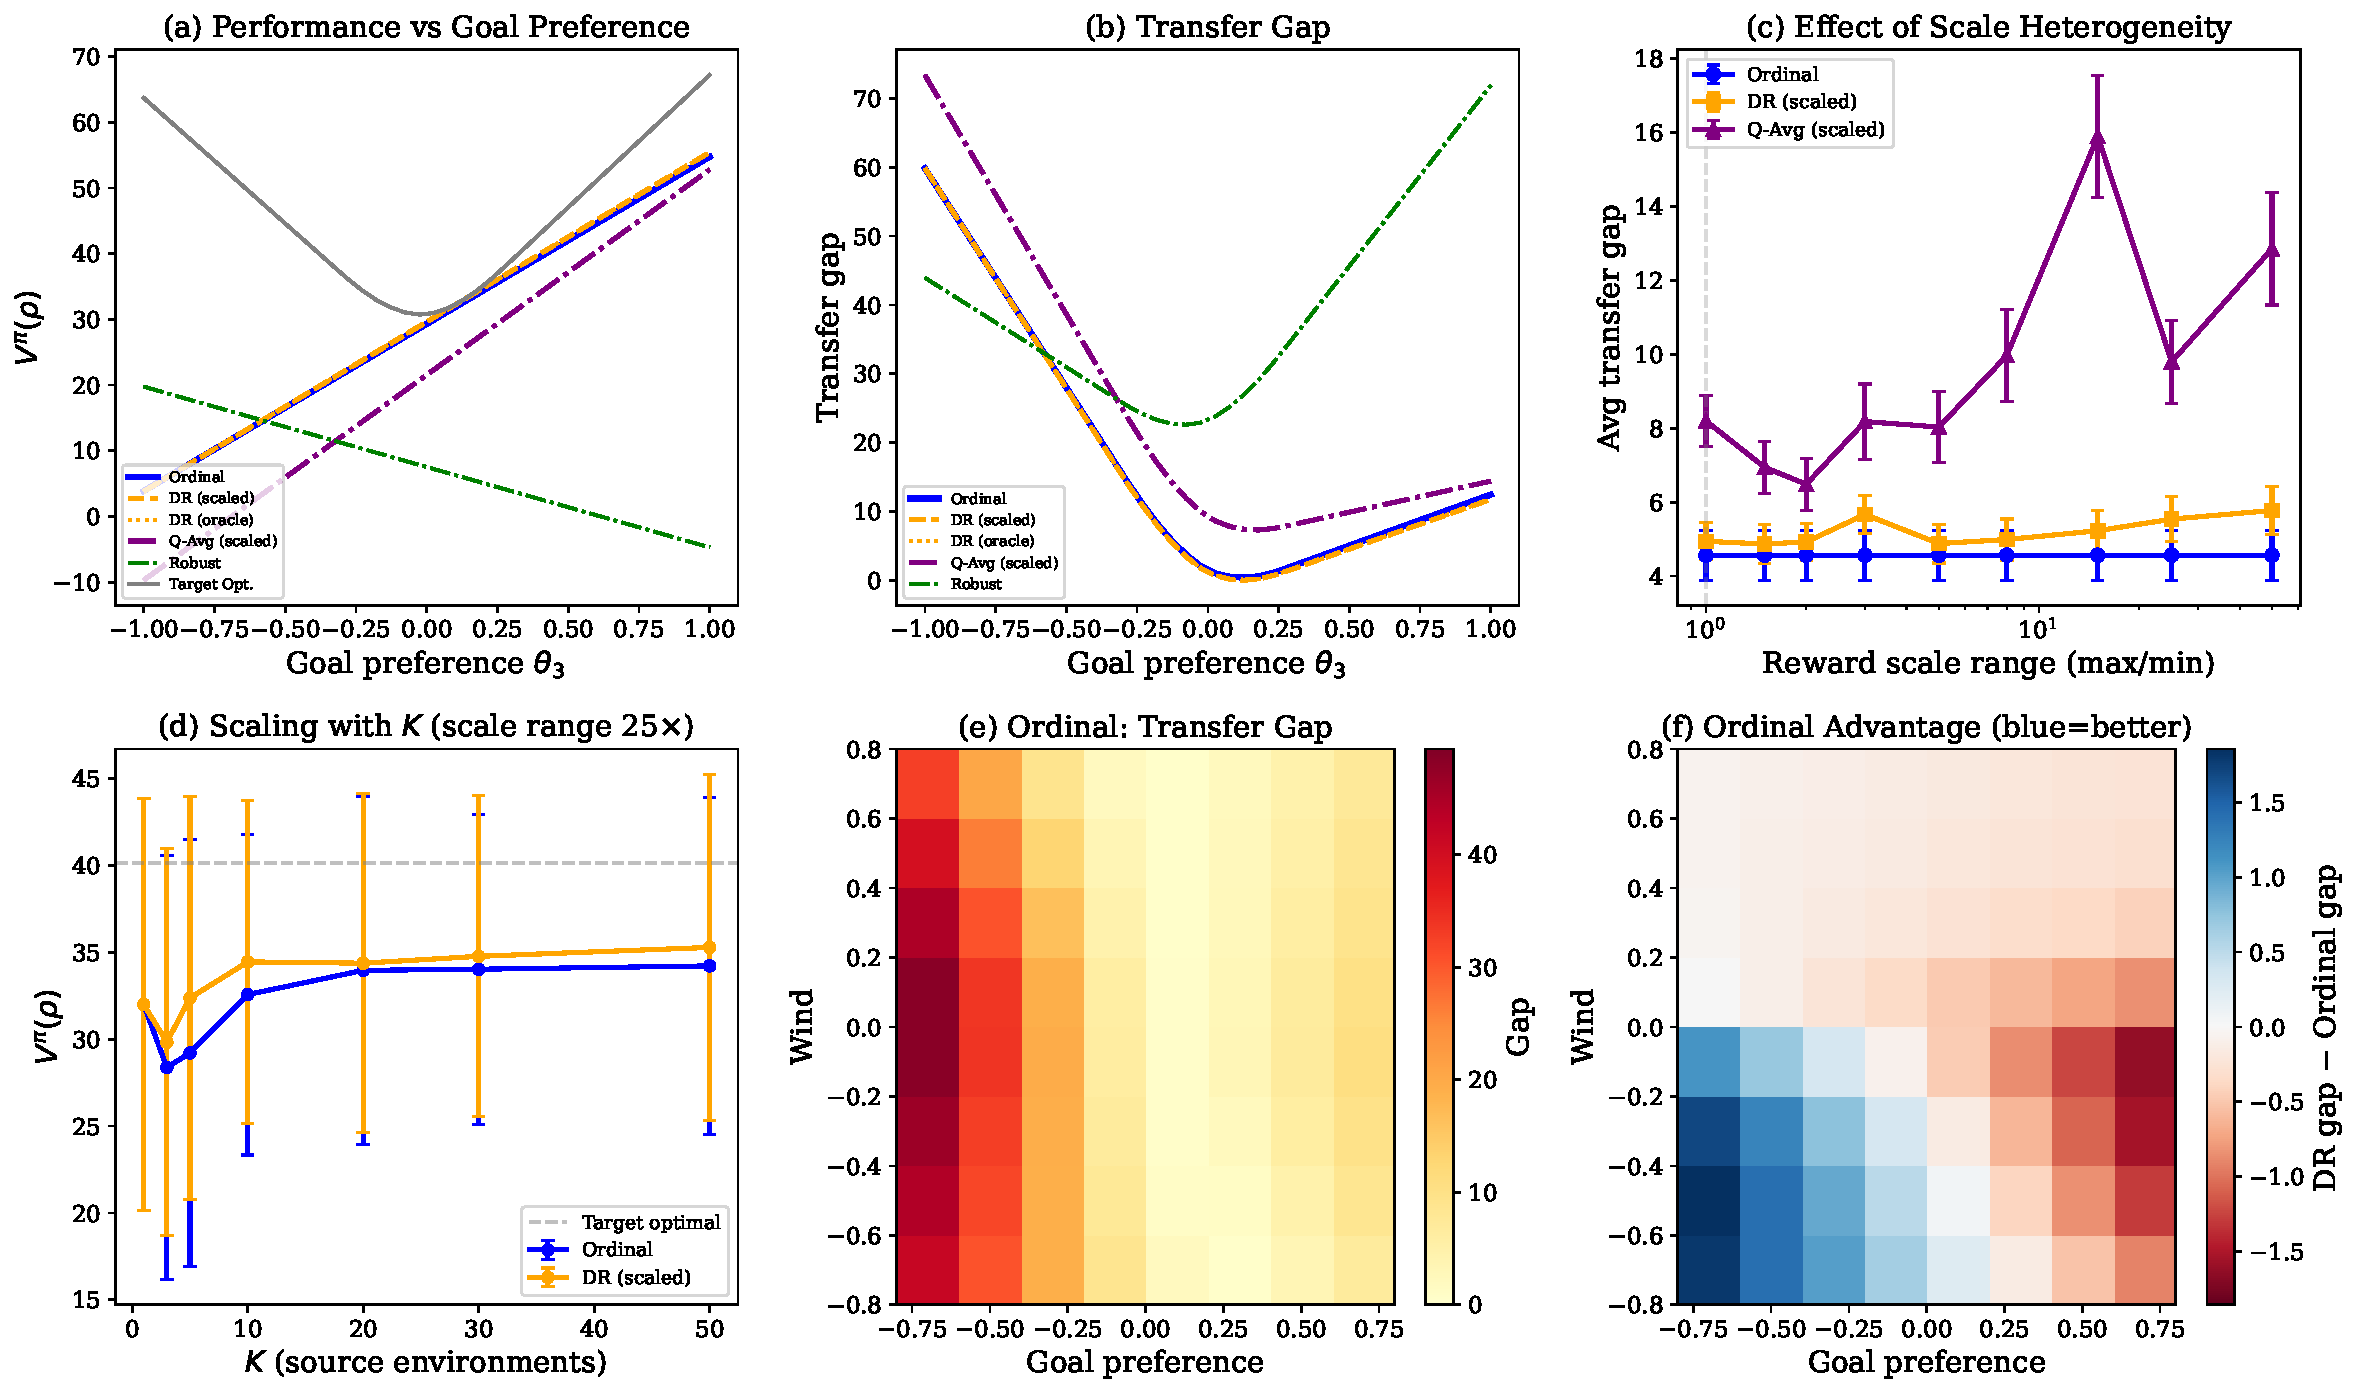
\includegraphics[width=\textwidth]{figures/exp6_baselines.pdf}
\caption{Baseline comparison on $10 \times 10$ grid with heterogeneous reward scales. (a) Performance vs.\ goal preference. (b) Transfer gap. (c) Ordinal gap is flat (scale-invariant) while Q-Averaging and DR degrade with scale heterogeneity. (d) Scaling with $K$. (e) Ordinal gap heatmap. (f) Ordinal advantage over DR (blue = ordinal better).}
\label{fig:baselines}
\end{figure}

% ────────────────────────────────────────────────────────────
\subsection{Neural Policy Transfer: DQN, Gymnasium, and MuJoCo}
\label{sec:exp-neural}
% ────────────────────────────────────────────────────────────

We now test whether ordinal transfer extends to \emph{neural} policies trained from scratch, across three settings of increasing complexity.

\paragraph{Discrete CartPole (DQN).}
\label{sec:exp-dqn}
DQN agents (2-layer MLP, 64 units) on 4-action CartPole (forces $\{-10,-3,+3,+10\}$\,N) at 6 gravities in $[6, 19]$\,m/s$^2$. Directional OC between the source ($g{=}9.8$) and LQR-optimal decays smoothly from $\approx 0.95$ to $\approx 0.75$; majority vote maintains agreement $=1.0$ up to $100\times$ rescaling, while Q-averaging drops to $0.81$ (Figure~\ref{fig:dqn}, Appendix~\ref{app:additional-exp}).

\paragraph{Gymnasium benchmarks (unmodified).}
\label{sec:exp-gymnasium-benchmark}
\texttt{CartPole-v1} (discrete, DQN, 3 seeds, 11 gravities) and \texttt{Pendulum-v1} (continuous, analytical LQR, 20 gravities) rule out custom-environment artifacts. On CartPole-v1, ensemble-averaged OC declines with $|\Delta g|$ and majority vote holds $=1.0$ up to $500\times$ rescaling while Q-averaging degrades (Figure~\ref{fig:gym-bench}, top). On Pendulum-v1, the transfer gap grows with log-log slope $\approx 1.88$ and gain/action displacement are linear in $|\Delta g|$, matching Theorems~\ref{thm:quadratic-subopt}--\ref{thm:action-displacement} (Figure~\ref{fig:gym-bench}, bottom).

\begin{figure}[t]
\centering
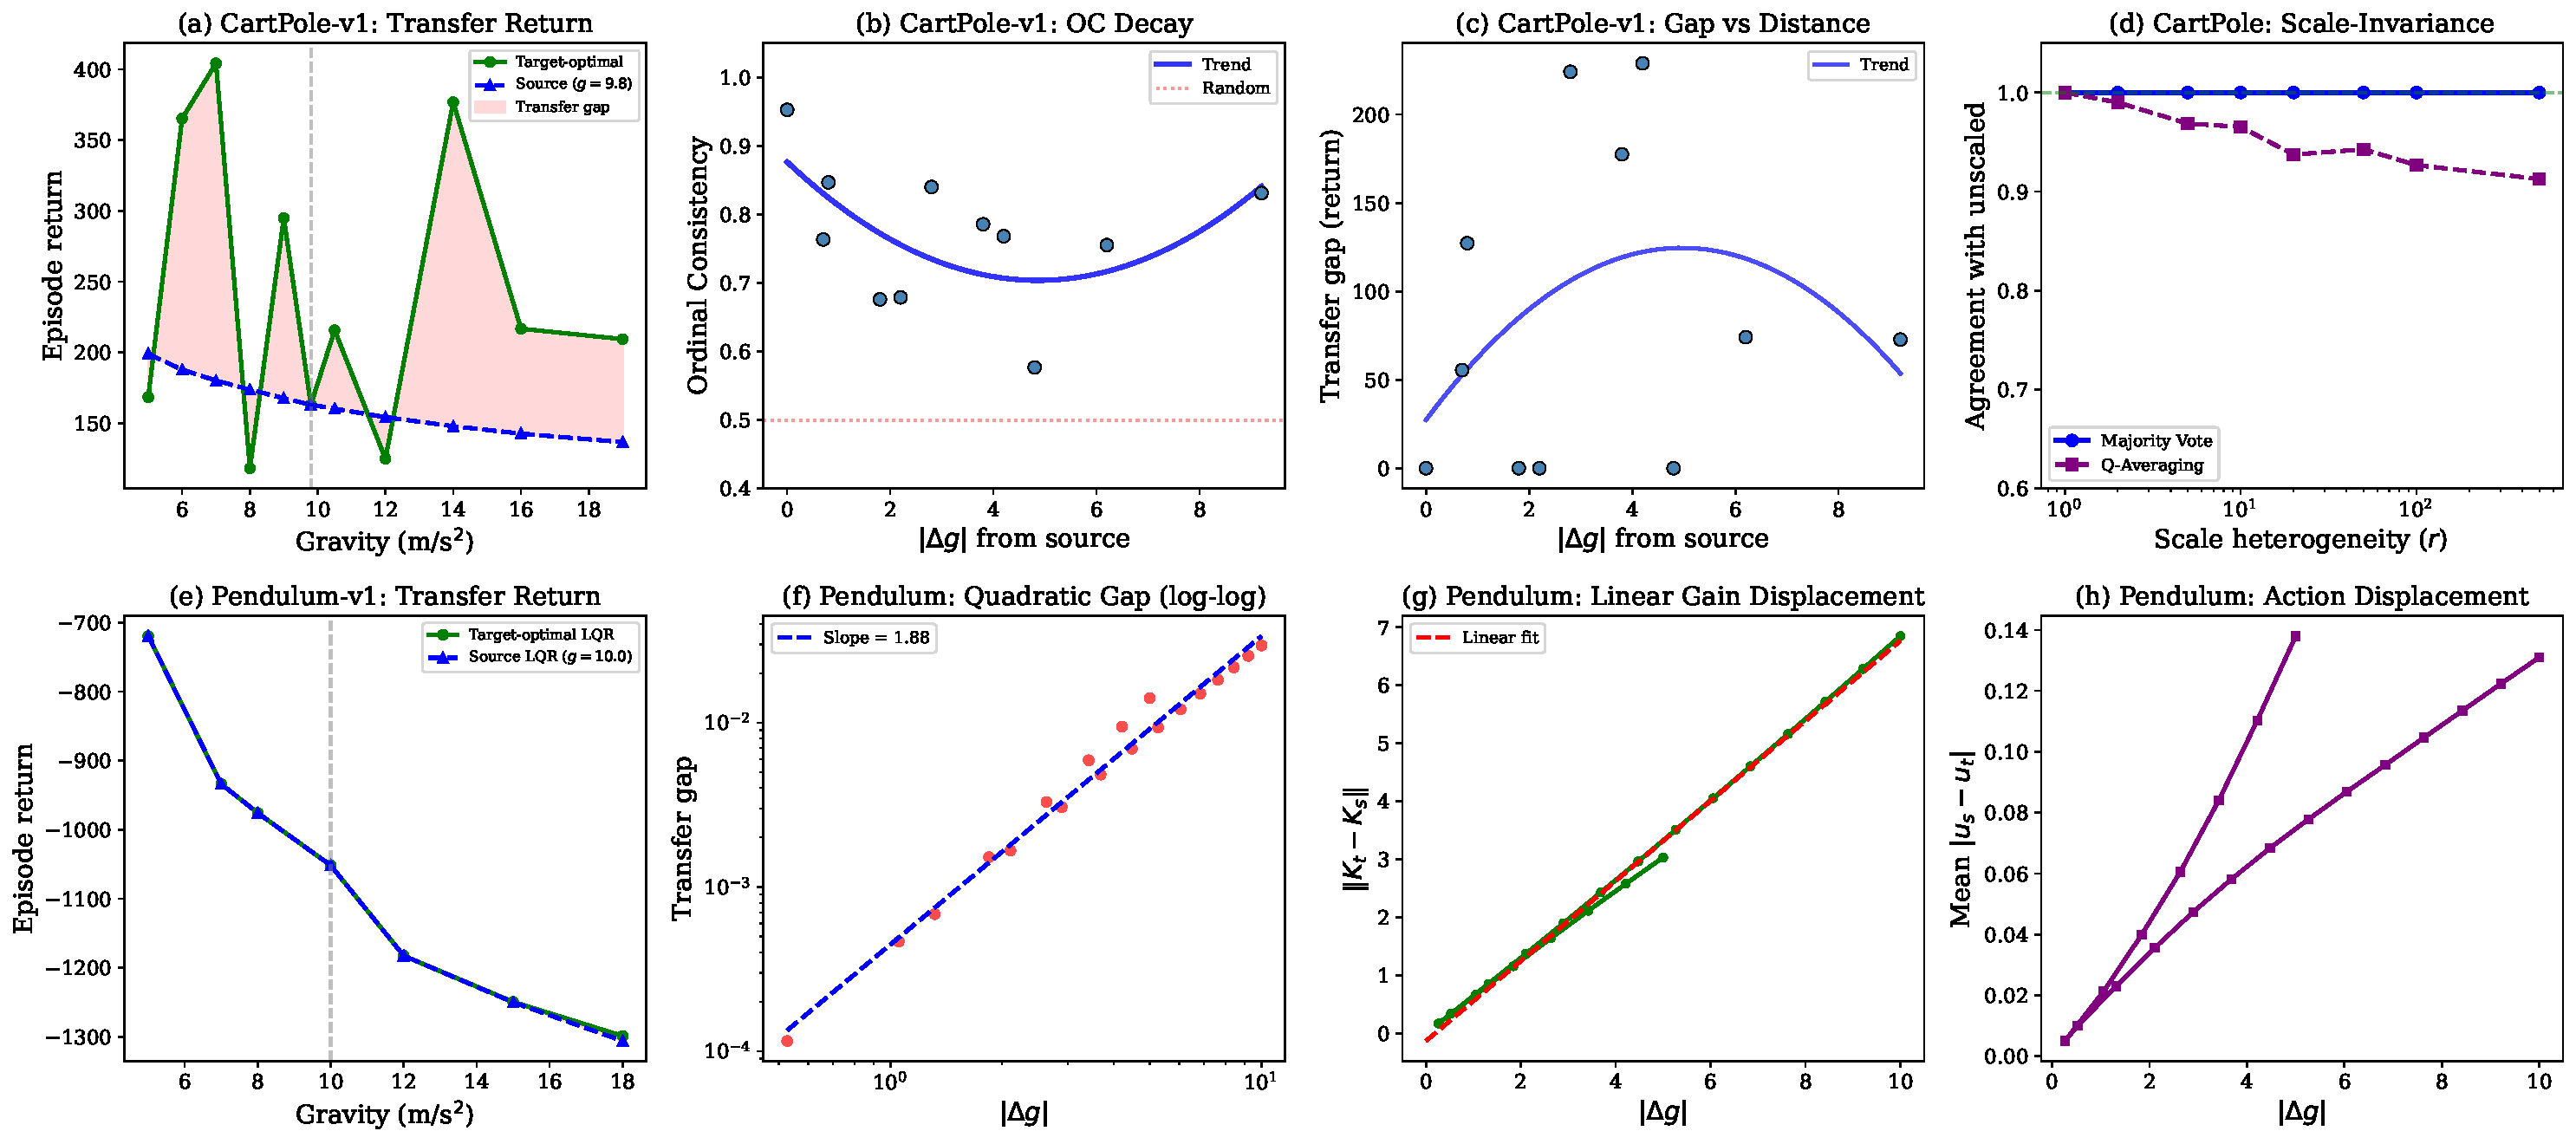
\includegraphics[width=\textwidth]{figures/exp9_gymnasium_benchmark.pdf}
\caption{Gymnasium benchmarks. Top: CartPole-v1 (discrete). (a)~Transfer return. (b)~OC trend. (c)~Gap. (d)~Scale-invariance. Bottom: Pendulum-v1 (continuous). (f)~Quadratic gap ($\approx 1.88$). (g)--(h)~Linear displacement.}
\label{fig:gym-bench}
\end{figure}

\paragraph{MuJoCo continuous control (SAC).}
\label{sec:exp-mujoco-transfer}
SAC (Stable-Baselines3, 500K steps) on HalfCheetah-v4 (17D/6D), Ant-v4 (27D/8D), Hopper-v4 (11D/3D) at $g \in \{5,7,9.81,12,15\}$\,m/s$^2$, plus a domain-randomization (DR) baseline over $[5,15]$. Figure~\ref{fig:mujoco-transfer}: \emph{transfer return} degrades smoothly (Hopper steepest, narrow single-leg region); \emph{directional OC} is highest for Ant ($0.75$--$0.79$, least decay), asymmetric for HalfCheetah, and lowest for Hopper ($0.60$--$0.69$, most decay), matching Theorem~\ref{thm:violation-growth}; \emph{scale-invariance}: MV $=1.000$ uniformly while MA falls to $0.70$--$0.87$. \emph{Transfer-gap scaling} (cross-seed mean over seeds $\{42,123,7\}$, Table~\ref{tab:slope-comparison}) stays strictly below the quadratic upper bound of Theorem~\ref{thm:continuous-bound-main} on Hopper ($\approx 1.17$) and HalfCheetah ($\approx 1.20$), the two environments where Assumption~\ref{asm:local-sc} remains valid across the target gravity range. Ant gives $\approx 2.52$, exceeding the bound; Appendix~\ref{app:hessian-diag} traces this to a directional precondition failure at light gravities, so Ant marks the boundary of the theorem's regime rather than refuting it. DR wins at extreme shifts (it trained there); single-gravity agents stay competitive at moderate shifts.

\paragraph{$F_\kappa$ as a neural diagnostic.} From 500 on-policy states per SAC model, Hopper's median gap ($\tilde{\kappa}=0.015$) is ${\sim}20\times$ smaller than Ant's ($0.363$) or HalfCheetah's ($0.258$), consistent with the coarse OC fragility ordering across environments (Figure~\ref{fig:fkappa-neural}). For quantitative prediction, however, median-only summaries are insufficient: Appendix~\ref{app:fkappa-bound} validates Theorem~\ref{thm:violation-growth} on all 12 (env, target) pairs and shows that, after a single per-environment scale calibration, the full CDF shape $\hat F_\kappa(c^* \cdot |\Delta g|)$ explains the measured violation $2.6\times$--$22\times$ better in MSE than a best-fit median-only predictor (Table~\ref{tab:shape-vs-median}), because the latter collapses to a step.

\paragraph{Multi-seed variance.} Across seeds $\{42,123,7\}$, directional-OC decay is stable (std $\leq 0.15$ per cell) and the qualitative claims reproduce. Transfer-gap magnitudes are noisier per seed: occasional $(\text{seed},g)$ cells where the source incidentally matches the target produce non-positive raw gaps that clip to a floor of $1$ before log fitting, and a single such event can shift a 5-point per-seed slope by several units (per-seed std $2.4$--$3.4$ across envs). We therefore aggregate at the cell level before fitting: the cross-seed mean of cell gaps cancels these zero-gap incidents within a cell and is the only stable summary. The headline Ant slope ($\approx 2.52$) is this cross-seed-mean slope, not the per-seed median ($1.72$, contaminated by the seed-$42$ clipping at $g{=}5$ where source returns collapse to $143\pm72$ vs.\ target $1{,}723\pm404$); reporting the median would mask the directional-precondition failure of Appendix~\ref{app:hessian-diag}. Full tables and per-seed breakdowns: Appendix~\ref{app:multiseed}.

\begin{figure}[t]
\centering
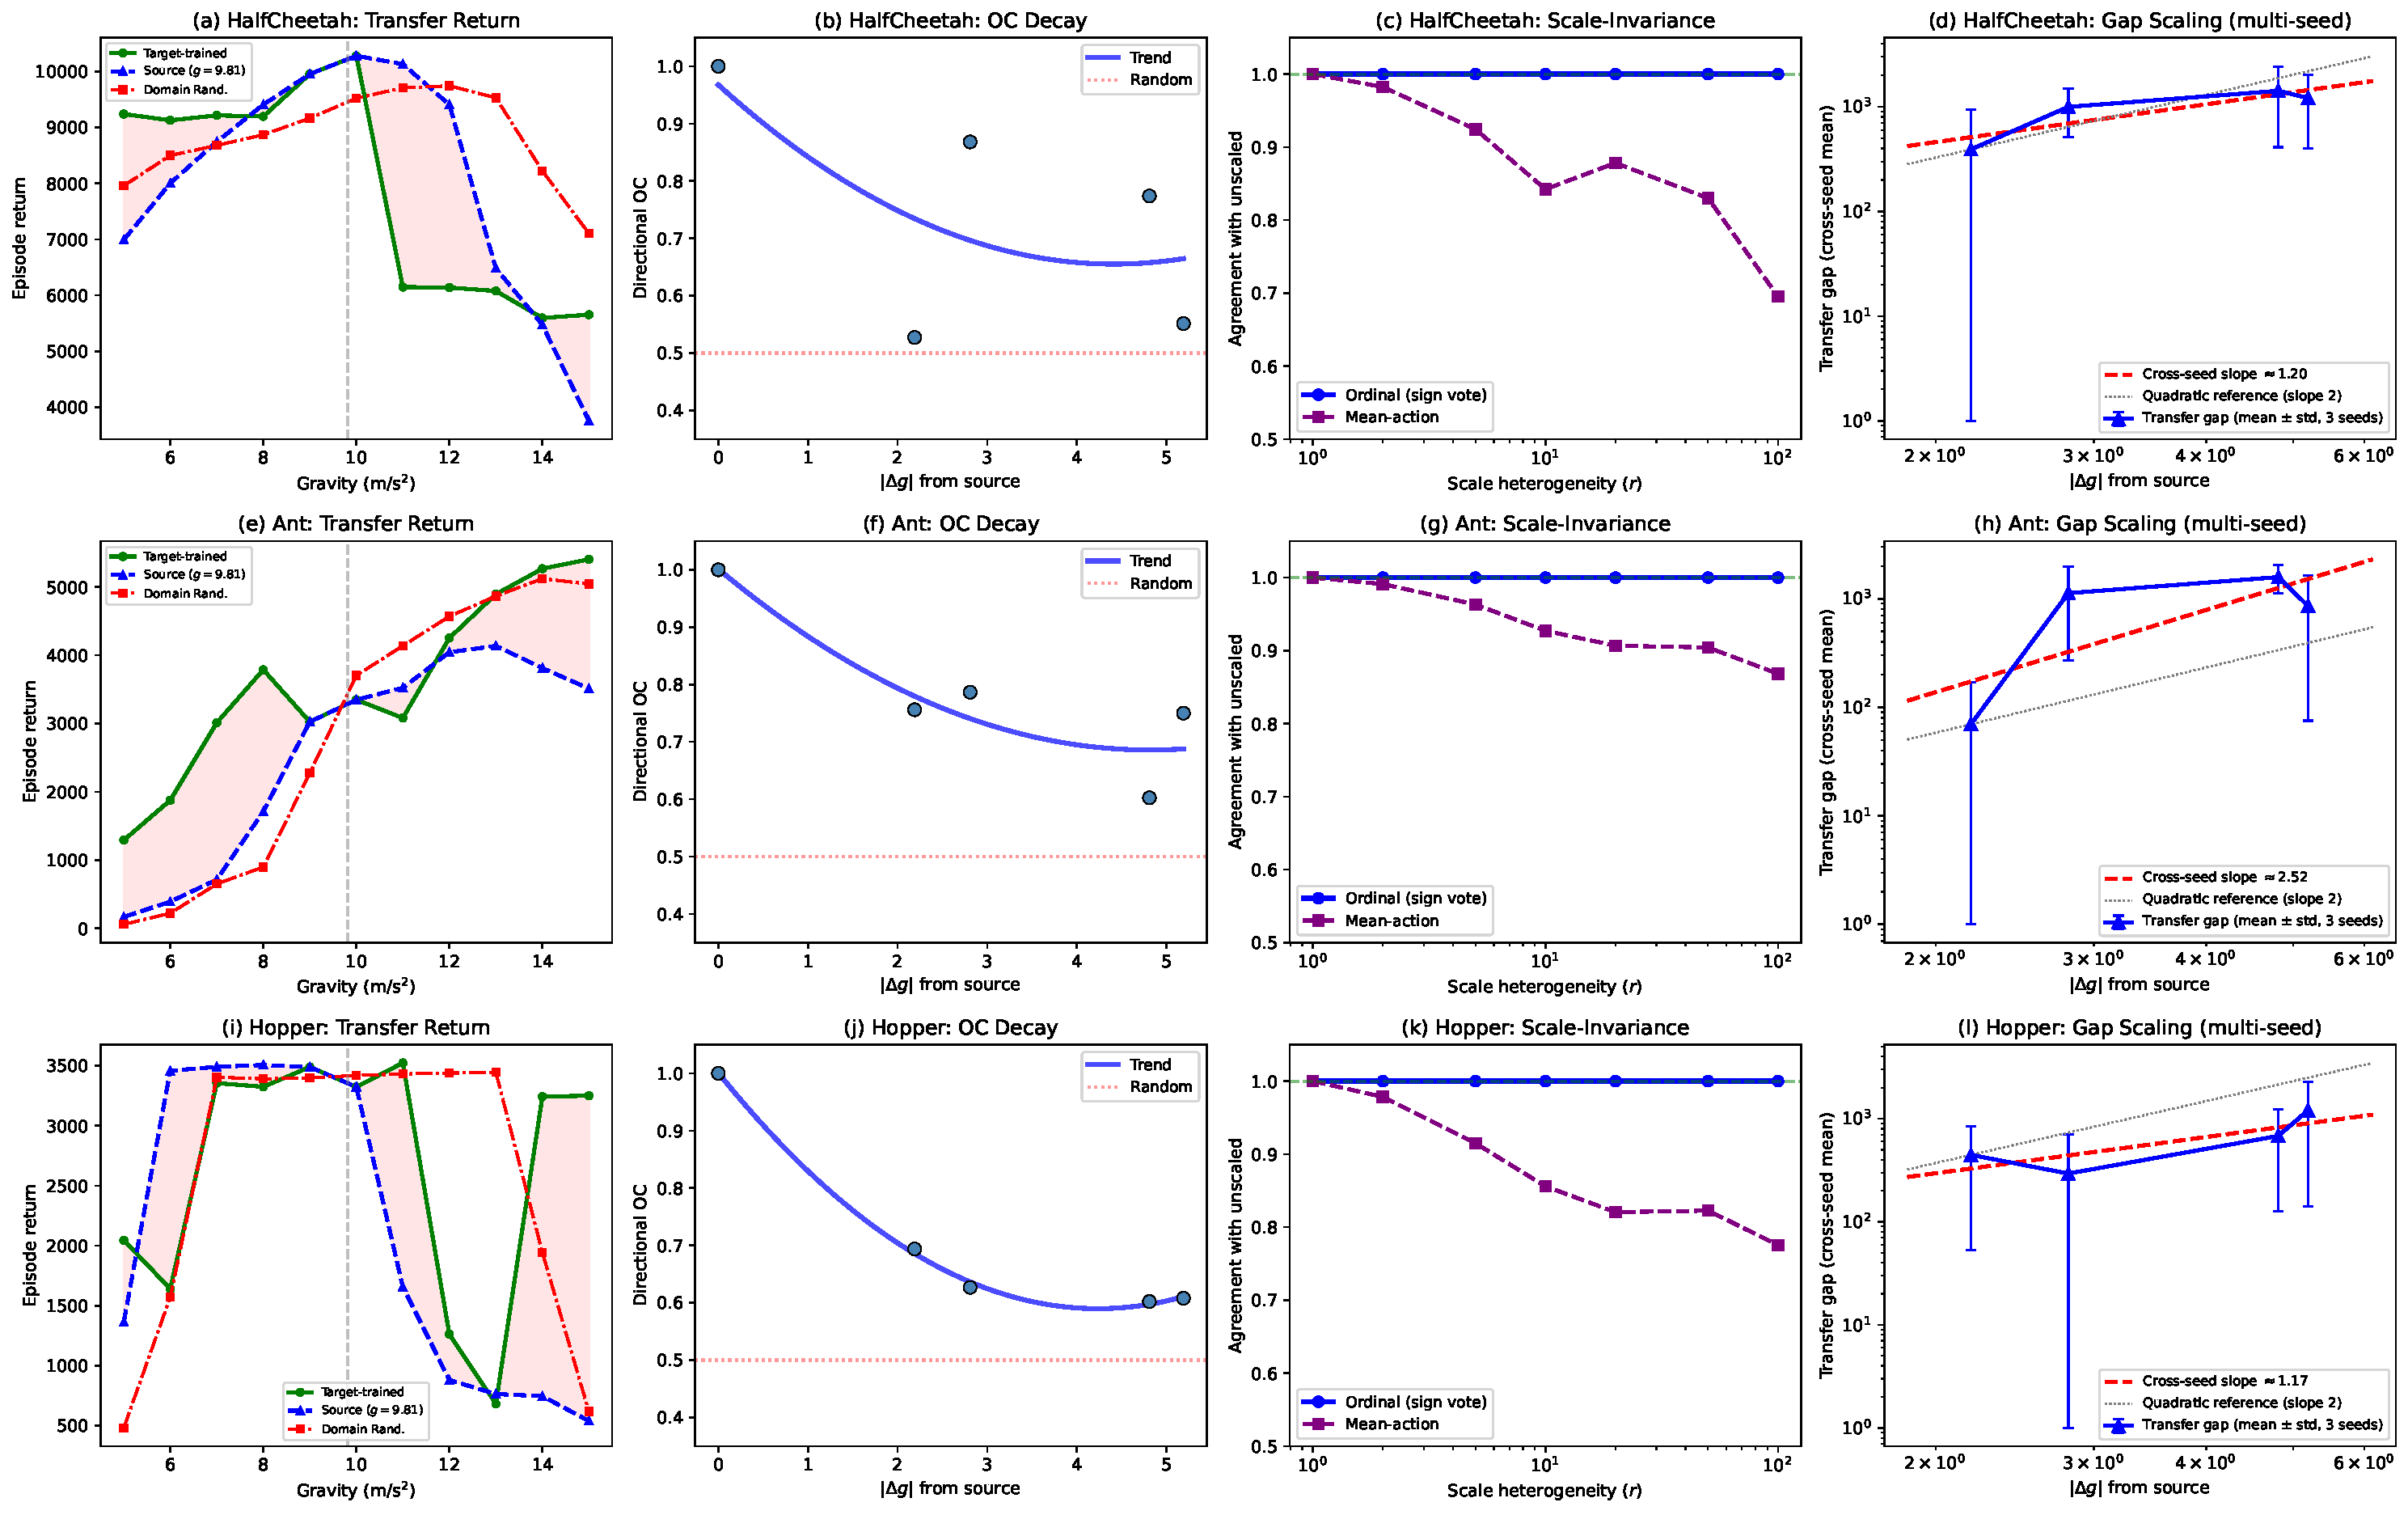
\includegraphics[width=0.68\textwidth]{figures/exp10_mujoco_transfer.pdf}
\caption{MuJoCo SAC (500K). Rows: HalfCheetah, Ant, Hopper. Cols: transfer return at seed $42$ (DR dashed), directional OC at seed $42$, scale-invariance at seed $42$ (MV $=1.000$; MA degrades), and transfer-gap scaling using cross-seed-mean cell-level gaps over seeds $\{42, 123, 7\}$ (error bars $\pm 1$ std). The gap-panel slope labels are the cross-seed fits ($1.20/2.52/1.17$ for HalfCheetah/Ant/Hopper) used as the headline numbers in the body and in Table~\ref{tab:slope-comparison}; the gray dotted line marks the quadratic reference (slope $2$). Under this summary, HalfCheetah and Hopper remain below the quadratic upper bound of Thm.~\ref{thm:continuous-bound-main}, while Ant exceeds it; Appendix~\ref{app:hessian-diag} traces the Ant deviation to a directional precondition failure at light gravities. Seed-$42$ single-fit slopes ($4.56/4.19/1.88$) are reported alongside the Hessian diagnostic in Appendix~\ref{app:hessian-diag} for the regime where the local quadratic model collapses.}
\label{fig:mujoco-transfer}
\end{figure}

\paragraph{Multi-dimensional parameter transfer.} Appendix~\ref{app:exp-multidim} extends the above to $d{=}3$ simultaneous shifts (gravity $\times$ friction $\times$ mass) on HalfCheetah-v4: the source policy stays competitive across all shift magnitudes, and OC decay, scale-invariance, and action displacement depend only on $\|\Delta\thetavec\|$ regardless of which physics parameters vary.

\paragraph{Source-only deploy-or-adapt decision.} A diagnostic is useful only if it improves decisions. For each target gravity $g \neq g_\mathrm{src}$ we decide at source time whether to deploy the source policy zero-shot or fall back to a domain-randomized policy trained on $g\in[5,15]$, scoring the decision by the resulting return. The rule adapts iff $\hat F_\kappa(c\,|\Delta g|) > \tau$ with env-agnostic $c=0.1, \tau=0.5$ (no per-env tuning); $\hat F_\kappa$ is the same source-side CDF used everywhere else. Inline summary (mean return over four non-source gravities, $\hat F_\kappa$ rule vs.\ \emph{always-deploy} / \emph{always-adapt} (DR) / oracle): \textbf{HalfCheetah} $\mathbf{8{,}194}$ vs.\ $7{,}143/8{,}396/8{,}396$; \textbf{Ant} $\mathbf{2{,}509}$ vs.\ $2{,}197/2{,}561/2{,}642$; \textbf{Hopper} $\mathbf{1{,}988}$ vs.\ $1{,}555/1{,}988/2{,}266$. The rule attains $75\%$ decision accuracy vs.\ oracle in all three envs, captures ${>}94\%$ of the oracle return, and strictly beats \emph{always-deploy} everywhere; unlike \emph{always-adapt} it correctly flags Ant $g{=}7$ (where the source policy is the better deployment) from source data alone. Per-cell breakdown and the full table: Appendix~\ref{app:deploy-or-adapt}.

% ============================================================

% ============================================================
\section{Related Work}
\label{sec:related}
% ============================================================

\textbf{Sim-to-real and transfer RL.} Domain randomization~\citep{tobin2017domain, peng2018sim, openai2019solving, mehta2020active}, system identification~\citep{ljung1998system, yu2017preparing, yu2019sim}, and rapid motor adaptation~\citep{kumar2021rma} all rely on cardinal value information; surveys~\citep{taylor2009transfer} cover task mapping and reward shaping. We show that argmax-only information, without cardinal critic estimates on the target, is sufficient for zero-shot deployment whenever the action-gap CDF $F_\kappa$ stays light-tailed near zero, with quantitative degradation bounds (Theorem~\ref{thm:violation-growth}) once it does not.

\textbf{Robust and Meta-RL.} Worst-case optimization~\citep{iyengar2005robust, nilim2005robust, panaganti2022robust} hedges against the uncertainty set; meta-RL~\citep{finn2017model, rakelly2019efficient, duan2016rl2} addresses \emph{how} to adapt. Our stability radius is complementary: it characterizes \emph{when} no robustness or adaptation is needed, and can gate the deploy-vs.-adapt decision.

\textbf{MDP sensitivity.} The Simulation~\citep{kearns2002near} and Performance Difference~\citep{kakade2002approximately, schulman2015trust} Lemmas bound value differences; parametric-MDP sensitivity is classical~\citep{schweitzer1968perturbation, cao2007stochastic}. We apply Bellman sensitivity (Proposition~\ref{prop:sensitivity}) to \emph{Q-gaps}, yielding ordinal certificates.

\textbf{Bisimulation metrics.} Bisimulation metrics and ordinal consistency address different invariance targets. Bisimulation asks whether two states remain close in value under all actions, typically through reward and transition similarity~\citep{ferns2004metrics, castro2020scalable}. Ordinal consistency instead asks whether the action ordering, and in particular the identity of the argmax action, is preserved. Neither notion implies the other: two environments can be far apart in value while preserving the same action ordering, and conversely can be value-close while swapping the top two actions. Since a greedy policy depends on the latter, ordinal consistency is the more relevant notion for zero-shot transfer without adaptation.

\textbf{Action gap and monotone comparative statics.} The action gap $\kappa$ controls sample complexity in a \emph{single} MDP~\citep{farahmand2011action} and drives exploration bonuses~\citep{bellemare2016increasing} as a \emph{pointwise} quantity. We instead study the \emph{distribution} $F_\kappa$ across states, a population-level question the worst-case $\min_s \kappa(s)$ cannot address since it discards shape information (flat vs.\ steep near zero) that governs graceful vs.\ catastrophic degradation. Topkis' theorem~\citep{topkis1998supermodularity, milgrom1994monotone} guarantees monotone actions under lattice structure; OC is strictly weaker, requiring only ordering preservation.

\textbf{Preference-based RL.} PbRL~\citep{christiano2017deep, wirth2017survey} and RLHF~\citep{ouyang2022training} learn from noisy human ordinal judgments. In our framework, ordinal information arises deterministically from the structural regularity of physics, enabling stability certificates (\S\ref{sec:stability}) that are unavailable with noisy preferences.

% ============================================================
\section{Discussion and Limitations}
\label{sec:discussion}
% ============================================================

\textbf{Summary.} The Ordinal MDP framework formalizes policy transfer under physics variation via ordinal consistency. The central result (Theorem~\ref{thm:violation-growth}) expresses the violation fraction through the action-gap CDF $F_\kappa$, explaining structurally why some environments tolerate large parameter shifts. Matching constructions (Propositions~\ref{prop:tight-growth},~\ref{prop:tight-growth-gamma}) saturate the bound to factor $1$ for every $\gamma \in [0,1)$. For continuous actions, local strong concavity (Assumption~\ref{asm:local-sc}) yields quadratic degradation where the assumption holds; Proposition~\ref{prop:model-free} gives a source-side data-driven OC certificate.

\textbf{On assumptions.} Only Lipschitz continuity (Assumption~\ref{asm:lipschitz}) is needed for Theorems~\ref{thm:transfer-gap},~\ref{thm:violation-growth},~\ref{thm:stability-radius}; differentiability (Assumption~\ref{asm:smooth}) is used only for the tight radius, and the continuous-action triplet (Assumptions~\ref{asm:local-sc}--\ref{asm:interior}) is automatic in LQR.

\textbf{Limitations.} (i) \emph{Local} radius: qualitative changes (e.g., contact switches) violate OC globally. (ii) Worst-case $L_Q{=}L_R/(1{-}\gamma)$ overestimates flips ($5.2\times$ at $\gamma{=}0.99$, Appendix~\ref{app:gamma-tightness}); Proposition~\ref{prop:lq-estimator} bounds $L_Q$ from the source ensemble. (iii) Proposition~\ref{prop:lq-estimator} bounds $L_Q$ from finite differences on the source ensemble but still requires the user to supply a curvature constant $H_Q$ and a Q-estimation tolerance $\varepsilon_Q$; both are interpretable but neither is purely data-driven. The certificate is therefore source-side rather than fully model-free, and is valid only on the support visited by the source ensemble; out-of-support shifts require either re-estimation or a domain-knowledge bound on $H_Q$. (iv) The $|\cS|{\cdot}|\cA|^2$ union bound extends to continuous states via $\epsilon$-covering (Appendix~\ref{app:covering-number}). (v) Theorem~\ref{thm:continuous-bound-main} is single-basin; the cross-seed-mean log-log slope stays below the quadratic upper bound on HalfCheetah ($1.20$) and Hopper ($1.17$), but exceeds it on Ant ($2.52$), driven by a directional precondition failure at light gravities (Appendix~\ref{app:hessian-diag}); a multi-basin / direction-aware extension is the main open direction. \textbf{Broader impact.} Certifying sim-to-real transfer reduces real-world fine-tuning; no negative societal impacts anticipated.

% ============================================================
% References
% ============================================================
\bibliographystyle{plainnat}
\bibliography{references}

% ============================================================
\newpage
\appendix
% ============================================================

\section{Complete Proofs}
\label{app:proofs}

\subsection{Proof of Lemma~\ref{lem:q-lipschitz} (Lipschitz \texorpdfstring{$Q^*_\theta$}{Q*})}

\begin{lemma}[Lipschitz $Q^*_\theta$]
\label{lem:q-lipschitz}
Under Assumption~\ref{asm:lipschitz}: $\|Q^*_{\theta_1} - Q^*_{\theta_2}\|_\infty \leq L_Q\|\theta_1 - \theta_2\|$ with $L_Q = \frac{L_R + \gamma|\cS|L_P\Vmax}{1-\gamma}$.
\end{lemma}

Let $T_\theta$ be the Bellman optimality operator: $(T_\theta Q)(s,a) = R_\theta(s,a) + \gamma\sum_{s'}P_\theta(s'|s,a)\max_{a'}Q(s',a')$.

For any $Q$:
\begin{align}
|(T_{\theta_1}Q)(s,a) - (T_{\theta_2}Q)(s,a)| &\leq |R_{\theta_1}(s,a) - R_{\theta_2}(s,a)| + \gamma\sum_{s'}|P_{\theta_1}(s'|s,a) - P_{\theta_2}(s'|s,a)|\cdot\|Q\|_\infty \nonumber\\
&\leq L_R\|\theta_1 - \theta_2\| + \gamma|\cS|L_P\|Q\|_\infty\|\theta_1 - \theta_2\|.
\end{align}
Since $Q^*_\theta = T_\theta Q^*_\theta$ is a fixed point and $T_\theta$ is a $\gamma$-contraction:
\begin{align}
\|Q^*_{\theta_1} - Q^*_{\theta_2}\|_\infty &= \|T_{\theta_1}Q^*_{\theta_1} - T_{\theta_2}Q^*_{\theta_2}\|_\infty \nonumber\\
&\leq \|T_{\theta_1}Q^*_{\theta_1} - T_{\theta_1}Q^*_{\theta_2}\|_\infty + \|T_{\theta_1}Q^*_{\theta_2} - T_{\theta_2}Q^*_{\theta_2}\|_\infty \nonumber\\
&\leq \gamma\|Q^*_{\theta_1} - Q^*_{\theta_2}\|_\infty + (L_R + \gamma|\cS|L_P\Vmax)\|\theta_1 - \theta_2\|.
\end{align}
Solving: $\|Q^*_{\theta_1} - Q^*_{\theta_2}\|_\infty \leq \frac{L_R + \gamma|\cS|L_P\Vmax}{1-\gamma}\|\theta_1 - \theta_2\| = L_Q\|\theta_1 - \theta_2\|$.

\subsection{Bellman Sensitivity and Tight Stability Radius}

\begin{assumption}[Differentiability]
\label{asm:smooth}
$\theta \mapsto R_\theta(s,a)$ and $\theta \mapsto P_\theta(s'|s,a)$ are $C^1$ for all $(s,a,s')$.
\end{assumption}

\begin{proposition}[Bellman Sensitivity Equation]
\label{prop:sensitivity}
Under Assumption~\ref{asm:smooth}, for $\theta$ where $\pi^*_\theta$ is locally constant, the Q-value sensitivity $\mathbf{s}_\theta = \frac{d\,\mathrm{vec}(Q^*_\theta)}{d\theta}$ satisfies:
\begin{equation}
\mathbf{s}_\theta = (\mathbf{I} - \gamma\mathbf{T}_{\theta,\pi})^{-1}\mathbf{b}_\theta, \quad \text{where } b_\theta(s,a) = \frac{\partial R_\theta(s,a)}{\partial\theta} + \gamma\sum_{s'}\frac{\partial P_\theta(s'|s,a)}{\partial\theta}V^*_\theta(s').
\end{equation}
\end{proposition}

\begin{theorem}[Tight Stability Radius]
\label{thm:tight-stability}
Under Assumptions~\ref{asm:lipschitz}--\ref{asm:smooth}, with $\sigma_\theta(s,a,a') = s_\theta(s,a) - s_\theta(s,a')$:
\begin{equation}
\rho_{\mathrm{tight}}(\theta_0) = \min_{s \in \cS}\;\min_{a \neq a'} \frac{|G_{\theta_0}(s,a,a')|}{\sup_{\theta \in \Theta_{\mathrm{reg}}}|\sigma_\theta(s,a,a')|} \geq \rho_{\mathrm{cons}}(\theta_0).
\end{equation}
\end{theorem}

\paragraph{Proof of Proposition~\ref{prop:sensitivity}.}
At $\theta$ where $\pi^*_\theta$ is locally constant, the Bellman equation reads:
$Q^*_\theta(s,a) = R_\theta(s,a) + \gamma\sum_{s'}P_\theta(s'|s,a)Q^*_\theta(s', \pi^*_\theta(s'))$.
Differentiating both sides with respect to $\theta$ (valid since $\pi^*_\theta$ is constant in a neighborhood):
\begin{equation}
\frac{\partial Q^*_\theta(s,a)}{\partial\theta} = \frac{\partial R_\theta(s,a)}{\partial\theta} + \gamma\sum_{s'}\frac{\partial P_\theta(s'|s,a)}{\partial\theta}V^*_\theta(s') + \gamma\sum_{s'}P_\theta(s'|s,a)\frac{\partial Q^*_\theta(s', \pi^*_\theta(s'))}{\partial\theta}.
\end{equation}
In matrix form with $\mathbf{s}_\theta = \mathrm{vec}(\partial Q^*_\theta/\partial\theta)$ and transition matrix $T_{\theta,\pi}$:
$\mathbf{s}_\theta = \mathbf{b}_\theta + \gamma\mathbf{T}_{\theta,\pi}\mathbf{s}_\theta$,
hence $\mathbf{s}_\theta = (\mathbf{I} - \gamma\mathbf{T}_{\theta,\pi})^{-1}\mathbf{b}_\theta$. The inverse exists since $\gamma < 1$ and $\mathbf{T}_{\theta,\pi}$ is a sub-stochastic matrix.

\subsection{Continuous Transfer Bound (stated informally in \S\ref{sec:continuous})}

\begin{theorem}[Continuous Transfer Bound]
\label{thm:continuous-bound}
Under Assumptions~\ref{asm:local-sc}--\ref{asm:interior}, for $\|\theta - \theta_0\|$ sufficiently small:
\[
V^*_{\theta}(\rho) - V^{\pi_0}_{\theta}(\rho) \leq \frac{L_{aa}\Lambda_{\max}^2}{2\mu^2(1-\gamma)}\|\theta - \theta_0\|^2, \qquad \Lambda_{\max} = \max_s \Lambda(s).
\]
\end{theorem}
\begin{proof}
Combine Theorem~\ref{thm:quadratic-subopt} (quadratic suboptimality, below) with Theorem~\ref{thm:action-displacement} (action displacement) to get $\Delta_\theta(s) \leq \tfrac{L_{aa}\Lambda_{\max}^2}{2\mu^2}\|\theta - \theta_0\|^2$. Substituting into Theorem~\ref{thm:transfer-gap} and summing visitation yields the bound.
\end{proof}

\subsection{Proof of Theorem~\ref{thm:quadratic-subopt} (Quadratic Suboptimality)}

\begin{theorem}[Quadratic Suboptimality]
\label{thm:quadratic-subopt}
Under Assumptions~\ref{asm:local-sc}--\ref{asm:interior}, for $\|\theta - \theta_0\|$ sufficiently small:
\[
\frac{\mu}{2}\|a^*_{\theta}(s) - a^*_{\theta_0}(s)\|^2 \leq \Delta_{\theta}(s) \leq \frac{L_{aa}}{2}\|a^*_{\theta}(s) - a^*_{\theta_0}(s)\|^2.
\]
\end{theorem}

Fix $s$ and $\theta$. Let $a^* = a^*_{\theta}(s)$ and $a_0 = a^*_{\theta_0}(s)$. By optimality, $\nabla_a Q^*_{\theta}(s, a^*) = 0$. Taylor expanding around $a^*$:
\begin{equation}
Q^*_{\theta}(s, a_0) = Q^*_{\theta}(s, a^*) + \frac{1}{2}(a_0 - a^*)^\top \nabla^2_{aa}Q^*_{\theta}(s, \tilde{a})(a_0 - a^*)
\end{equation}
for some $\tilde{a}$ on the segment $[a_0, a^*]$. By Assumption~\ref{asm:local-sc}:
$-\frac{L_{aa}}{2}\|a_0 - a^*\|^2 \leq Q^*_{\theta}(s, a_0) - Q^*_{\theta}(s, a^*) \leq -\frac{\mu}{2}\|a_0 - a^*\|^2$.
Since $\Delta_{\theta}(s) = Q^*_{\theta}(s, a^*) - Q^*_{\theta}(s, a_0)$, the result follows.

\subsection{Optimal Action Sensitivity and Action Displacement}

\begin{theorem}[Optimal Action Sensitivity]
\label{thm:action-sensitivity}
Under Assumptions~\ref{asm:local-sc}--\ref{asm:interior}:
\[
\frac{\partial a^*_\theta(s)}{\partial\theta} = -[\nabla^2_{aa}Q^*_\theta(s, a^*_\theta(s))]^{-1}\;\nabla^2_{a\theta}Q^*_\theta(s, a^*_\theta(s)).
\]
\end{theorem}
\begin{proof}
The first-order condition at an interior optimum is $\nabla_a Q^*_\theta(s, a^*_\theta(s)) = 0$. Define $F(\theta, a) = \nabla_a Q^*_\theta(s, a)$. By Assumption~\ref{asm:local-sc}, $\frac{\partial F}{\partial a} = \nabla^2_{aa}Q^*_\theta$ is invertible. The implicit function theorem~\citep{krantz2002implicit} gives $\frac{da^*_\theta(s)}{d\theta} = -[\partial F/\partial a]^{-1}[\partial F/\partial\theta] = -[\nabla^2_{aa}Q^*_\theta]^{-1}\nabla^2_{a\theta}Q^*_\theta$.
\end{proof}

\begin{theorem}[Action Displacement Bound]
\label{thm:action-displacement}
Under Assumptions~\ref{asm:local-sc}--\ref{asm:interior}:
\[
\|a^*_{\theta}(s) - a^*_{\theta_0}(s)\| \leq \frac{\Lambda(s)}{\mu}\|\theta - \theta_0\|, \qquad \Lambda(s) = \sup_\theta\|\nabla^2_{a\theta}Q^*_\theta(s,a^*_\theta(s))\|_{\mathrm{op}}.
\]
\end{theorem}
\begin{proof}
Integrate the sensitivity bound of Theorem~\ref{thm:action-sensitivity} along the straight line from $\theta_0$ to $\theta$. By Assumption~\ref{asm:local-sc}, $\|[\nabla^2_{aa}Q^*_\theta]^{-1}\|_{\mathrm{op}} \leq 1/\mu$, and by definition $\|\nabla^2_{a\theta}Q^*_\theta\|_{\mathrm{op}} \leq \Lambda(s)$.
\end{proof}

\subsection{Proof of Theorem~\ref{thm:sample-complexity} (Discrete Sample Complexity)}

\begin{theorem}[Discrete Sample Complexity]
\label{thm:sample-complexity}
The majority-vote ordinal policy $\hat{\pi}(s) = \argmax_a \sum_{k=1}^K \ind[\pi^*_{\theta_k}(s) = a]$ recovers the population-optimal ordering at every state with probability $\geq 1 - \delta$ if $K \geq \frac{1}{2\kappa_{\min}^2}\ln\frac{|\cS|\binom{|\cA|}{2}}{\delta}$.
\end{theorem}

\begin{corollary}[Noise Robustness]
\label{cor:noisy-q}
If $\|\hat{Q}_{\theta_k} - Q^*_{\theta_k}\|_\infty \leq \epsilon_Q$ and the minimum nonzero Q-gap $g_{\min} > 2\epsilon_Q$, then substituting $\hat{Q}$ for $Q^*$ preserves all ordinal comparisons.
\end{corollary}

\begin{proof}[Proof of Theorem~\ref{thm:sample-complexity}]
For each pair $(s, a, a')$ with $a \neq a'$, define $X_k = \ind[G_{\theta_k}(s,a,a') > 0]$. These are i.i.d.\ Bernoulli with mean $p_{s,a,a'} = \Prob_{\theta \sim \mu}[G_\theta(s,a,a') > 0]$. By Definition~\ref{def:pop-margin}, $|p_{s,a,a'} - 1/2| \geq \kappa_{\min}$.

The majority vote errs on $(s,a,a')$ when $\frac{1}{K}\sum_k X_k$ is on the wrong side of $1/2$. By Hoeffding:
$\Prob\left[\left|\frac{1}{K}\sum_k X_k - p_{s,a,a'}\right| \geq \kappa_{\min}\right] \leq 2\exp(-2K\kappa_{\min}^2)$.
Union-bounding over all $|\cS|\binom{|\cA|}{2}$ pairs and setting $2|\cS|\binom{|\cA|}{2}\exp(-2K\kappa_{\min}^2) \leq \delta$ gives $K \geq \frac{1}{2\kappa_{\min}^2}\ln\frac{2|\cS|\binom{|\cA|}{2}}{\delta}$. Corollary~\ref{cor:noisy-q} follows from the triangle inequality: $|\hat{G}_{\theta_k} - G_{\theta_k}| \leq 2\epsilon_Q$, so $g_{\min} > 2\epsilon_Q$ preserves the sign of every nonzero gap.
\end{proof}

\subsection{Continuous Sample Complexity}

\begin{theorem}[Continuous Sample Complexity]
\label{thm:continuous-sample}
The mean-action policy $\bar{a}(s) = \frac{1}{K}\sum_{k=1}^K a^*_{\theta_k}(s)$ satisfies:
\[
\E_{\theta}[\Delta_{\theta}(s)] \leq \frac{L_{aa}}{2}\left(\Var_\mu[a^*_\theta(s)] + \frac{D^2 m}{K}\right),
\]
where $D = \sup_\theta \|a^*_\theta(s) - \E_\mu[a^*_\theta(s)]\|$ and $m = \dim(\cA)$.
\end{theorem}
\begin{proof}
Let $\mu^* = \E_\mu[a^*_\theta(s)]$. Decompose $\bar{a} - \mu^* = \frac{1}{K}\sum_k (a^*_{\theta_k} - \mu^*)$; by independence, $\E[\|\bar{a}-\mu^*\|^2] \leq \Var_\mu[a^*_\theta]/K$. Combining with the bias term $\|\mu^* - a^*_\theta(s)\|^2 \leq D^2$ and applying Theorem~\ref{thm:quadratic-subopt} (quadratic suboptimality) with the Hessian bound $-L_{aa}I$ gives the claim.
\end{proof}

\section{Ordinal Transfer Algorithm}
\label{app:algorithm}

Algorithm~\ref{alg:ordinal-transfer} operationalizes the Source-Agreement Certificate (Proposition~\ref{prop:model-free}) together with the following corollary:

\begin{corollary}[Within-Support Transfer Certificate]
\label{cor:model-free-transfer}
If $\hat{\kappa} > 0$, then for any $\theta \in \operatorname{supp}(\mu)$ with $\|\theta - \theta_0\| < \hat{\kappa}/(2L_Q)$, the transfer gap is zero: $V^*_{\theta}(\rho) = V^{\pi_0}_{\theta}(\rho)$. For $\theta \notin \operatorname{supp}(\mu)$, the same conclusion holds only if $L_Q$ is known to bound the sensitivity uniformly along the straight-line path from $\theta_0$ to $\theta$ (Lipschitz extrapolation).
\end{corollary}

\begin{algorithm}[h]
\caption{Ordinal Transfer: Deploy or Fine-Tune}
\label{alg:ordinal-transfer}
\begin{algorithmic}[1]
\REQUIRE Source parameter distribution $\mu$ over $\Theta$; number of source policies $K$; confidence $\delta \in (0,1)$; either $L_Q$ directly, or smoothness $H_Q$ + critic-error bound $\varepsilon_Q$ (Proposition~\ref{prop:lq-estimator}); target parameter $\theta$
\ENSURE Policy $\hat{\pi}$ for the target MDP $M_\theta$
\STATE \textbf{// Phase 1: Source Training \& Certificate}
\FOR{$k = 1, \ldots, K$}
  \STATE Sample $\theta_k \sim \mu$; train $\pi^*_{\theta_k}$ to convergence on $M_{\theta_k}$
\ENDFOR
\STATE Compute pairwise agreement: $\hat{p}(s, a, a') \leftarrow \frac{1}{K}\sum_{k=1}^K \ind[G_{\theta_k}(s,a,a') > 0]$
\STATE Estimate ordinal margin: $\hat{\kappa} \leftarrow \min_{s,\, a \neq a'} |\hat{p}(s,a,a') - \tfrac{1}{2}| - \sqrt{\frac{\ln(2|\cS|\binom{|\cA|}{2}/\delta)}{2K}}$
\STATE Compute (or estimate via Prop.~\ref{prop:lq-estimator}) $L_Q$ upper bound $\bar L_Q$; set radius $\hat{\rho} \leftarrow \hat{\kappa}\, /\, (2\bar L_Q)$
\STATE \textbf{// Phase 2: Deploy or Fine-Tune}
\IF{$\hat{\kappa} > 0$ \AND $\theta \in \operatorname{supp}(\mu)$ \AND $\|\theta - \theta_0\| < \hat{\rho}$}
  \STATE \textbf{Deploy (certified):} $\hat{\pi} \leftarrow \pi^*_{\theta_0}$ \hfill $\triangleright$ \emph{zero-shot transfer; gap $= 0$}
\ELSIF{$\hat{\kappa} > 0$ \AND $\|\theta - \theta_0\| < \hat{\rho}$ \AND user asserts $\bar L_Q$ valid along $[\theta_0, \theta]$}
  \STATE \textbf{Deploy (extrapolated):} $\hat{\pi} \leftarrow \pi^*_{\theta_0}$ \hfill $\triangleright$ \emph{requires Lipschitz extrapolation outside $\operatorname{supp}(\mu)$; not data-certified}
\ELSIF{$\hat{\kappa} > 0$}
  \STATE \textbf{Deploy with bound:} $\hat{\pi} \leftarrow \pi^*_{\theta_0}$  \hfill $\triangleright$ \emph{gap $\leq \frac{2\Vmax}{1-\gamma} \int_0^{2L_Q\|\theta-\theta_0\|} F_\kappa(x)\, dx$}
\ELSE
  \STATE \textbf{Fine-tune:} initialize from $\pi^*_{\theta_0}$, train on $M_\theta$ \hfill $\triangleright$ \emph{OC not certified}
\ENDIF
\RETURN $\hat{\pi}$
\end{algorithmic}
\end{algorithm}

\begin{remark}[Deploy decision]
\label{rem:deploy-decision}
In practice, the Deploy branches (Lines 9--14) of Algorithm~\ref{alg:ordinal-transfer} decide to deploy zero-shot when either the certified regime applies, or when the bounded regime gap is below a user-specified tolerance $\epsilon_{\mathrm{tol}}$. The tolerance is problem-specific (e.g., 5\% of $V^*_{\theta_0}$). When neither holds, Phase 2 falls through to fine-tuning, using $\pi^*_{\theta_0}$ as a warm start---this typically reduces sample complexity by an order of magnitude compared to training from scratch.
\end{remark}

\section{Proof of Proposition~\ref{prop:lq-estimator} (Source-Side $L_Q$ Estimator)}
\label{app:lq-estimator-proof}

\begin{proof}
Fix any $(s,a)$ and any $\theta \in [\theta_{\min}, \theta_{\max}]$. Since $\theta_1, \ldots, \theta_K$ span $\Theta$, there exists $k$ with $\theta \in [\theta_k, \theta_{k+1}]$. By the mean value theorem applied to the (assumed differentiable) map $\theta' \mapsto Q^*_{\theta'}(s,a)$ on $[\theta_k, \theta_{k+1}]$, there exists $\xi \in [\theta_k, \theta_{k+1}]$ with
\[
\partial_\theta Q^*_\xi(s,a) \;=\; \frac{Q^*_{\theta_{k+1}}(s,a) - Q^*_{\theta_k}(s,a)}{h_k}.
\]
Combining the critic-error bound $|\hat Q_{\theta_k} - Q^*_{\theta_k}| \leq \varepsilon_Q$ with the triangle inequality,
\[
|\partial_\theta Q^*_\xi(s,a)| \;\leq\; \frac{|\hat Q_{\theta_{k+1}}(s,a) - \hat Q_{\theta_k}(s,a)| + 2\varepsilon_Q}{h_k}.
\]
Since $|\partial^2_\theta Q^*_\theta| \leq H_Q$, the gradient $\partial_\theta Q^*$ is $H_Q$-Lipschitz in $\theta$, so
\[
|\partial_\theta Q^*_\theta(s,a)| \;\leq\; |\partial_\theta Q^*_\xi(s,a)| + H_Q |\theta - \xi| \;\leq\; \frac{|\hat Q_{\theta_{k+1}}(s,a) - \hat Q_{\theta_k}(s,a)| + 2\varepsilon_Q}{h_k} + H_Q h_k.
\]
Taking the supremum over $\theta \in \Theta$ (which selects some $k$) and over $(s,a)$ yields $L_Q \leq \hat L_Q^{\mathrm{cert}}$. Since $\hat L_Q^{\mathrm{cert}} \geq L_Q$, the inequality $\hat\rho := \hat\kappa/(2 \hat L_Q^{\mathrm{cert}}) \leq \hat\kappa/(2 L_Q)$ shows that substituting $\hat L_Q^{\mathrm{cert}}$ in place of $L_Q$ in Proposition~\ref{prop:model-free} yields a valid (and conservative) stability radius.
\end{proof}

\begin{remark}[Multi-dimensional $\theta$]
\label{rem:lq-multidim}
For $\Theta \subset \R^d$ with $d > 1$, the same argument yields a directional bound: for any unit vector $u$, $|u^\top \nabla_\theta Q^*_\theta(s,a)|$ is bounded as in~\eqref{eq:lq-cert} using ensemble pairs aligned with $u$. Combining $d$ linearly independent directions and applying $\|\nabla_\theta Q^*\| \leq \sqrt{d}\, \max_u |u^\top \nabla_\theta Q^*|$ recovers a bound on $L_Q$. In practice, physics-parameter sweeps used in our experiments are 1-d (gravity) or low-d ($d=3$ in Appendix~\ref{app:exp-multidim}), and the 1-d statement of Proposition~\ref{prop:lq-estimator} is what we evaluate empirically.
\end{remark}

\begin{remark}[Tightness of the inflation factor]
\label{rem:lq-inflation}
The two correction terms $2\varepsilon_Q/h_k$ and $H_Q h_k$ trade off through the spacing $h_k$: dense sampling reduces $H_Q h_k$ at the cost of inflating $2\varepsilon_Q/h_k$. The optimal $h_k = \sqrt{2\varepsilon_Q / H_Q}$ balances them. With our MuJoCo SAC ensemble at $\theta_k \in \{5, 7, 9.81, 12, 15\}$ (gravity), the largest gap is $h_{\max} = 3.00$ and the inflation $H_Q h_{\max}$ is observable directly from the second-order finite difference (Appendix~\ref{app:exp-lq}).
\end{remark}

\section{Tightness Example}
\label{app:tightness}

Consider $\cS = \{s_1, s_2\}$, $\cA = \{a_1, a_2\}$, $\gamma = 0.9$, $\theta \in [0, 0.5]$. Let $P_\theta(s_1|s_1,a_1) = 0.8+\theta$, $R_\theta(s_1,a_1) = 1$, and all other rewards zero. The Simulation Lemma bound is $\frac{2\cdot0.9\cdot10}{(0.1)^2}\cdot\theta = 1800\theta$, while our decomposition gives the exact gap, which is $O(\theta)$ with a constant roughly $0.5$, a ratio of $\sim 3{,}600\times$.

\section{Tight Violation Growth Bound for Continuous Actions}
\label{app:tight-violation}

Theorem~\ref{thm:violation-growth}(ii) uses the worst-case $\Vmax$ per violation state. For continuous actions, combining with Theorem~\ref{thm:quadratic-subopt} (quadratic suboptimality) and Theorem~\ref{thm:action-displacement} (action sensitivity) yields a tighter bound.

\begin{proposition}[Tight Violation Bound]
\label{prop:tight-violation}
Under Assumptions~\ref{asm:lipschitz}--\ref{asm:interior}, for states $s \in \Sviol$ with continuous actions:
\begin{equation}
\Delta_{\theta}(s) \leq \frac{L_{aa}}{2}\|a^*_{\theta}(s) - a^*_{\theta_0}(s)\|^2 \leq \frac{L_{aa}}{2}\|\Lambda(s)\|^2\|\theta - \theta_0\|^2 + O(\|\Delta\theta\|^3),
\end{equation}
where $\Lambda(s) = da^*_\theta(s)/d\theta|_{\theta_0}$ is the action sensitivity (Theorem~\ref{thm:action-sensitivity}). Substituting into Theorem~\ref{thm:transfer-gap}:
\begin{equation}
V^*_\theta(\rho) - V^{\pi_0}_\theta(\rho) \leq \frac{L_{aa}\bar{\Lambda}^2}{2(1-\gamma)} \cdot F_\kappa(2L_Q\|\Delta\theta\|) \cdot \|\Delta\theta\|^2,
\end{equation}
where $\bar{\Lambda}^2 = \max_{s \in \Sviol}\|\Lambda(s)\|^2$.
\end{proposition}

This separates the transfer gap into two factors: $F_\kappa$ controls \emph{how many} states violate OC (growing with $\|\Delta\theta\|$), and $\|\Delta\theta\|^2$ controls \emph{how much} each violation costs. For discrete actions, the per-state cost is $O(1)$ (step function), so the gap scales as $O(F_\kappa)$; for continuous actions, the per-state cost is $O(\|\Delta\theta\|^2)$, yielding faster-than-linear growth.

\section{Proof of Proposition~\ref{prop:tight-growth} (Tightness of Violation Growth)}
\label{app:tight-growth}

\begin{proposition}[Tightness of Violation Growth]
\label{prop:tight-growth}
For any action gap CDF $F_\kappa$ and any $\epsilon > 0$, there exists a Lipschitz MDP family with Q-Lipschitz constant $L_Q$ such that $|\Sviol(\theta_0, \theta)| / |\cS| \geq F_\kappa(2L_Q\|\Delta\theta\|) - \epsilon$.
\end{proposition}

\begin{corollary}[Transfer Gap Matching Lower Bound]
\label{cor:transfer-gap-lower}
For the construction below with uniform initial distribution and $\gamma = 0$:
\[
V^*_\theta(\rho) - V^{\pi_0}_\theta(\rho) = \int_0^{2L_Q\|\Delta\theta\|}\!\! F_\kappa(x)\, dx.
\]
\end{corollary}

We construct a Lipschitz MDP family that saturates the $F_\kappa$ bound.

\textbf{Construction.} Let $\cS = \{s_1, \ldots, s_n\}$, $\cA = \{a_1, a_2\}$, $\gamma = 0$, $\Theta = [-1, 1]$. For each state $s_i$, define action gaps $\kappa_i = \kappa(s_i, \theta_0)$ that match the given CDF $F_\kappa$. Set:
\begin{equation}
R_\theta(s_i, a_1) = \kappa_i/2 - L_R \cdot |\theta - \theta_0|, \quad R_\theta(s_i, a_2) = -\kappa_i/2 + L_R \cdot |\theta - \theta_0|,
\end{equation}
with transitions $P_\theta(s_j|s_i, a) = 1/n$ for all $s_j$ (uniform, $\theta$-independent). At $\theta_0$, $Q^*_{\theta_0}(s_i, a_1) - Q^*_{\theta_0}(s_i, a_2) = \kappa_i$ (since $\gamma = 0$), so $\pi^*_{\theta_0}(s_i) = a_1$. As $\theta$ shifts, the Q-gap at $s_i$ decreases at rate $2L_R$. Setting $L_Q = L_R$ (since $\gamma = 0$, $P$ is $\theta$-independent), the ordering at $s_i$ flips when $\kappa_i = 2L_Q|\theta - \theta_0|$, i.e., at $|\Delta\theta| = \kappa_i / (2L_Q)$.

\textbf{Violation count.} At shift $\|\Delta\theta\|$, every state with $\kappa_i \leq 2L_Q\|\Delta\theta\|$ has its ordering flipped. Therefore:
$|\Sviol| / |\cS| = |\{s_i : \kappa_i \leq 2L_Q\|\Delta\theta\|\}| / n = F_\kappa(2L_Q\|\Delta\theta\|)$.

This matches the upper bound in Theorem~\ref{thm:violation-growth}(i) with equality, establishing tightness up to $\epsilon$ (by taking $n$ large enough to approximate any CDF). The construction satisfies Assumption~\ref{asm:lipschitz} with $L_R = L_Q$ and $L_P = 0$.

\textbf{Transfer gap (Corollary~\ref{cor:transfer-gap-lower}).} In this construction, with uniform $\rho = (1/n, \ldots, 1/n)$ and $\gamma = 0$, the transfer gap is:
\begin{equation}
V^*_\theta(\rho) - V^{\pi_0}_\theta(\rho) = \frac{1}{n}\sum_{i:\, \kappa_i \leq t} (t - \kappa_i), \quad t = 2L_Q\|\Delta\theta\|.
\end{equation}
Letting $n \to \infty$ with $\kappa_i$ drawn from $F_\kappa$, this converges to $\int_0^t F_\kappa(x)\,dx$ by integration by parts: $\frac{1}{n}\sum_{i:\,\kappa_i \leq t}(t - \kappa_i) = \int_0^t (t - x)\,dF_\kappa(x) = \int_0^t F_\kappa(x)\,dx$. \qed

\begin{proposition}[Tightness of Violation Growth for $\gamma > 0$]
\label{prop:tight-growth-gamma}
Fix any $\gamma \in [0, 1)$, any worst-case Q-Lipschitz constant $L_Q > 0$, any action gap CDF $F_\kappa$ supported on $[0, \kappa_{\max}]$, and any $\epsilon > 0$. There exists a Lipschitz MDP family $\{M_\theta\}_{\theta \in [-1,1]}$ whose worst-case Q-Lipschitz constant equals $L_Q$ and whose action-gap CDF at $\theta_0 = 0$ matches $F_\kappa$ (up to $\epsilon$), such that
\[
\frac{|\Sviol(\theta_0, \theta)|}{|\cS|} \;\geq\; F_\kappa\!\left(2L_Q\|\theta - \theta_0\|\right) - \epsilon
\qquad \text{for all } \theta \in [-1,1].
\]
\end{proposition}

\begin{proof}
Take $n$ large enough that an empirical CDF over $n$ samples approximates $F_\kappa$ uniformly within $\epsilon/2$, and choose $\kappa_1, \ldots, \kappa_n \in [0, \kappa_{\max}]$ accordingly. Set $\cS = \{s_1, \ldots, s_n\} \cup \{s^+, s^-\}$, $\cA = \{a_1, a_2\}$, $\theta_0 = 0$. Pick $W \geq (1-\gamma)(\kappa_{\max} + 2L_Q)/\gamma$ and define $\theta$-independent rewards $R(s^+, \cdot) = W$, $R(s^-, \cdot) = -W$, $R(s_i, \cdot) = 0$, so the reward Lipschitz constant is $L_R = 0$. The terminal states $s^\pm$ are absorbing self-loops; transitions from each $s_i$ are $\theta$-dependent with
\[
P_\theta(s^+ \mid s_i, a_1) = \tfrac{1}{2} + \Delta_i(\theta), \qquad P_\theta(s^+ \mid s_i, a_2) = \tfrac{1}{2} - \Delta_i(\theta),
\]
and $P_\theta(s^- \mid s_i, a_k) = 1 - P_\theta(s^+ \mid s_i, a_k)$, where $\Delta_i(\theta) = \delta_i - c\,|\theta|$ with $\delta_i = \kappa_i(1-\gamma)/(4\gamma W)$ and $c = L_Q(1-\gamma)/(2\gamma W)$. The choice of $W$ guarantees $|\Delta_i(\theta)| \leq 1/2$ for every $i$ and $|\theta| \leq 1$, so transitions are valid probabilities; they are continuous in $\theta$ with transition Lipschitz constant $L_P = c$.

The absorbing values are $V^*(s^+) = W/(1-\gamma)$ and $V^*(s^-) = -W/(1-\gamma)$. At each $s_i$,
\[
Q^*_\theta(s_i, a_k) = (-1)^{k+1}\, \tfrac{2\gamma W}{1-\gamma}\,\Delta_i(\theta),
\qquad
Q^*_\theta(s_i, a_1) - Q^*_\theta(s_i, a_2) = \tfrac{4\gamma W}{1-\gamma}\Delta_i(\theta) = \kappa_i - 2L_Q|\theta|,
\]
using $4\gamma W \delta_i/(1-\gamma) = \kappa_i$ and $4\gamma W c/(1-\gamma) = 2L_Q$. The $\theta$-derivative of each $Q^*(s_i, a_k)$ has magnitude $2\gamma W c/(1-\gamma) = L_Q$; at $s^\pm$ the values are $\theta$-independent (Lipschitz $0$). Hence the worst-case Q-Lipschitz constant of the family equals $L_Q$.

At $\theta_0 = 0$ the action gap at $s_i$ equals $\kappa_i$, while $s^+$ and $s^-$ have two identical actions (both self-loops with the same reward), so their per-state action gap is $0$ and they never lie in $\Sviol$; the MDP's action-gap CDF is $[|\{i : \kappa_i \leq x\}| + 2\cdot\mathbf{1}[x \geq 0]]/(n+2)$, which agrees with $F_\kappa$ uniformly to within $\epsilon$ once $n$ is large. The ordering at $s_i$ flips iff $\kappa_i \leq 2L_Q|\theta|$, so
\[
\frac{|\Sviol(0, \theta)|}{|\cS|} = \frac{|\{i : \kappa_i \leq 2L_Q|\theta|\}|}{n+2} \geq F_\kappa(2L_Q|\theta|) - \epsilon. \qed
\]
\end{proof}

\begin{corollary}[Transfer Gap Matching Lower Bound for $\gamma > 0$]
\label{cor:transfer-gap-lower-gamma}
For the construction of Proposition~\ref{prop:tight-growth-gamma} with uniform initial distribution over the transient states, the transfer gap satisfies, in the limit $n \to \infty$,
\[
V^*_\theta(\rho) - V^{\pi_0}_\theta(\rho) = \int_0^{2L_Q\|\Delta\theta\|}\!\! F_\kappa(x)\, dx.
\]
\end{corollary}

\begin{proof}
For $s_i$ with $\kappa_i > 2L_Q|\theta|$ the source policy stays optimal and contributes zero. For $s_i \in \Sviol$ the source takes $a_1$ while the target-optimal action is $a_2$, so the per-state gap is $V^*_\theta(s_i) - V^{\pi_0}_\theta(s_i) = Q^*_\theta(s_i, a_2) - Q^*_\theta(s_i, a_1) = -(\kappa_i - 2L_Q|\theta|) = 2L_Q|\theta| - \kappa_i$. Averaging over $\rho$ and applying integration by parts as in Corollary~\ref{cor:transfer-gap-lower} gives the integral form. \qed
\end{proof}

The construction attains the worst-case Q-gap growth rate $2L_Q$ exactly, so the bound in Theorem~\ref{thm:violation-growth}(i) is tight to factor $1$ for every $\gamma \in [0, 1)$, matching the $\gamma = 0$ case of Corollary~\ref{cor:transfer-gap-lower}.

\begin{remark}[On the chain-MDP looseness in Appendix~\ref{app:gamma-tightness}]
\label{rem:gamma-positive-tightness}
Saturation requires the action-channel to translate worst-case $Q$ perturbations into worst-case $Q$-\emph{gap} perturbations, which either reward Lipschitz ($L_R > 0$) or transition Lipschitz ($L_P > 0$) can supply. The self-loop construction of Corollary~\ref{cor:transfer-gap-lower} uses the first channel and saturates at $\gamma = 0$; for $\gamma > 0$ self-loops alone cap the Q-gap rate at $2L_R$, short of $2L_Q$ by factor $(1-\gamma)^{-1}$. The construction above uses the transition channel instead ($L_R = 0$, $L_P > 0$) with action-dependent, $\theta$-varying transitions to a high/low-value pair, which reaches the full $2L_Q$. The $5.2\times$ empirical looseness on the 20-state chain at $\gamma = 0.99$ (Table~\ref{tab:gamma-tight}) is consistent with this: that family has $\theta$-independent transitions and reward perturbations that do not align to saturate the Q-gap rate, so plugging the worst-case $L_Q$ into the bound overestimates flips for that specific family. A separate cascade question (whether state-dependent transitions can amplify a single flip into $\Omega(|\cS|)$ secondary flips) remains open, but is no longer load-bearing for tightness.
\end{remark}

% ────────────────────────────────────────────────────────────
\section{Additional Experiments}
\label{app:additional-exp}
% ────────────────────────────────────────────────────────────

Experiments that validate the framework but are not essential to the main narrative are moved here for space. The main body keeps transfer gap decomposition (\S\ref{sec:exp-transfer-gap}), baseline comparison (\S\ref{sec:exp-baselines}), and neural-policy transfer (\S\ref{sec:exp-neural}).

\subsection{Ordinal Stability Radius (Theorem~\ref{thm:stability-radius}; tight version in \S\ref{app:proofs})}
\label{app:exp-stability}

\paragraph{Setup.} 8-state chain MDP with 3 actions. $\theta \in \R$ controls slip probability and reward. We compare the conservative radius (Thm.~\ref{thm:stability-radius}, using $2L_Q$) against the tight radius (Thm.~\ref{thm:tight-stability}, Appendix~\ref{app:proofs}, using $\sup_\theta|\sigma_\theta|$) and the empirical OC region.

\paragraph{Results.} Figure~\ref{fig:stability}(a): the tight radius is $20.8\times$ larger than the conservative one ($0.367$ vs.\ $0.018$), showing the practical benefit of Bellman sensitivity analysis. Both provide valid lower bounds on the true OC region. Figure~\ref{fig:stability}(c): per-state stability radii $\rho_s(\theta_0)$ correlate with action gaps $\kappa(s)$, as predicted by Definition~\ref{def:gap-cdf}.

\begin{figure}[h]
\centering
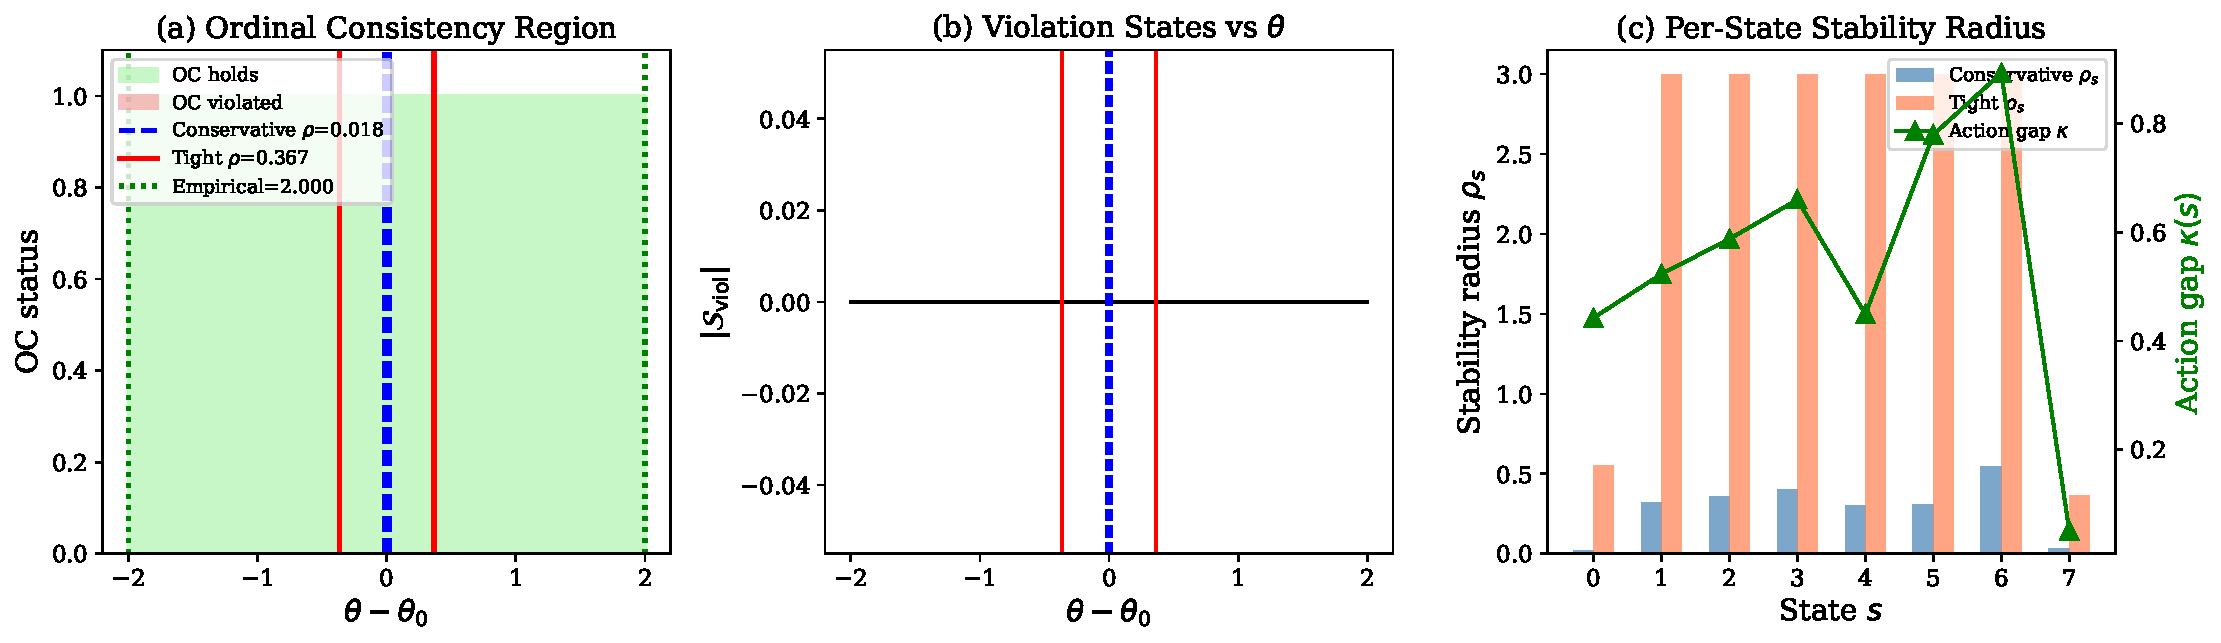
\includegraphics[width=\textwidth]{figures/exp2_stability_radius.pdf}
\caption{Ordinal stability radius. (a) OC region (green) with conservative (blue, $\rho = 0.018$) and tight (red, $\rho = 0.367$) radii. (b) Violation count. (c) Per-state radii track action gaps.}
\label{fig:stability}
\end{figure}

\subsection{Quadratic Degradation in LQR (Theorems~\ref{thm:quadratic-subopt}--\ref{thm:action-displacement}, Appendix~\ref{app:proofs})}
\label{sec:exp-lqr}

\paragraph{Setup.} 2D mass-spring-damper (LQR) with $\theta = (\text{stiffness}, \text{damping})$ perturbations from nominal. Source policy is optimal for $\theta_0 = (0,0)$.

\paragraph{Results.} Figure~\ref{fig:lqr}(b) (log-log) shows slope $\approx 2$ in all three perturbation directions, confirming Theorem~\ref{thm:quadratic-subopt} (Appendix~\ref{app:proofs}). The quadratic coefficients are $\alpha = 0.030$ (stiffness), $0.004$ (damping), $0.027$ (diagonal). The action displacement is linear in $\|\Delta\theta\|$ (Figure~\ref{fig:lqr}(c)--(d), slope $\approx 1.0$), consistent with Theorem~\ref{thm:action-displacement} (Appendix~\ref{app:proofs}). The strong concavity parameter is $\mu = L_{aa} = 0.134$ (condition number 1), matching LQR theory where $\nabla^2_{uu}Q^* = -(R + \gamma B^\top P B)$. Figure~\ref{fig:lqr}(f) illustrates the three degradation regimes from our theory: zero gap within the stability radius, quadratic growth for continuous actions, and a step function for discrete actions.

\begin{figure}[h]
\centering
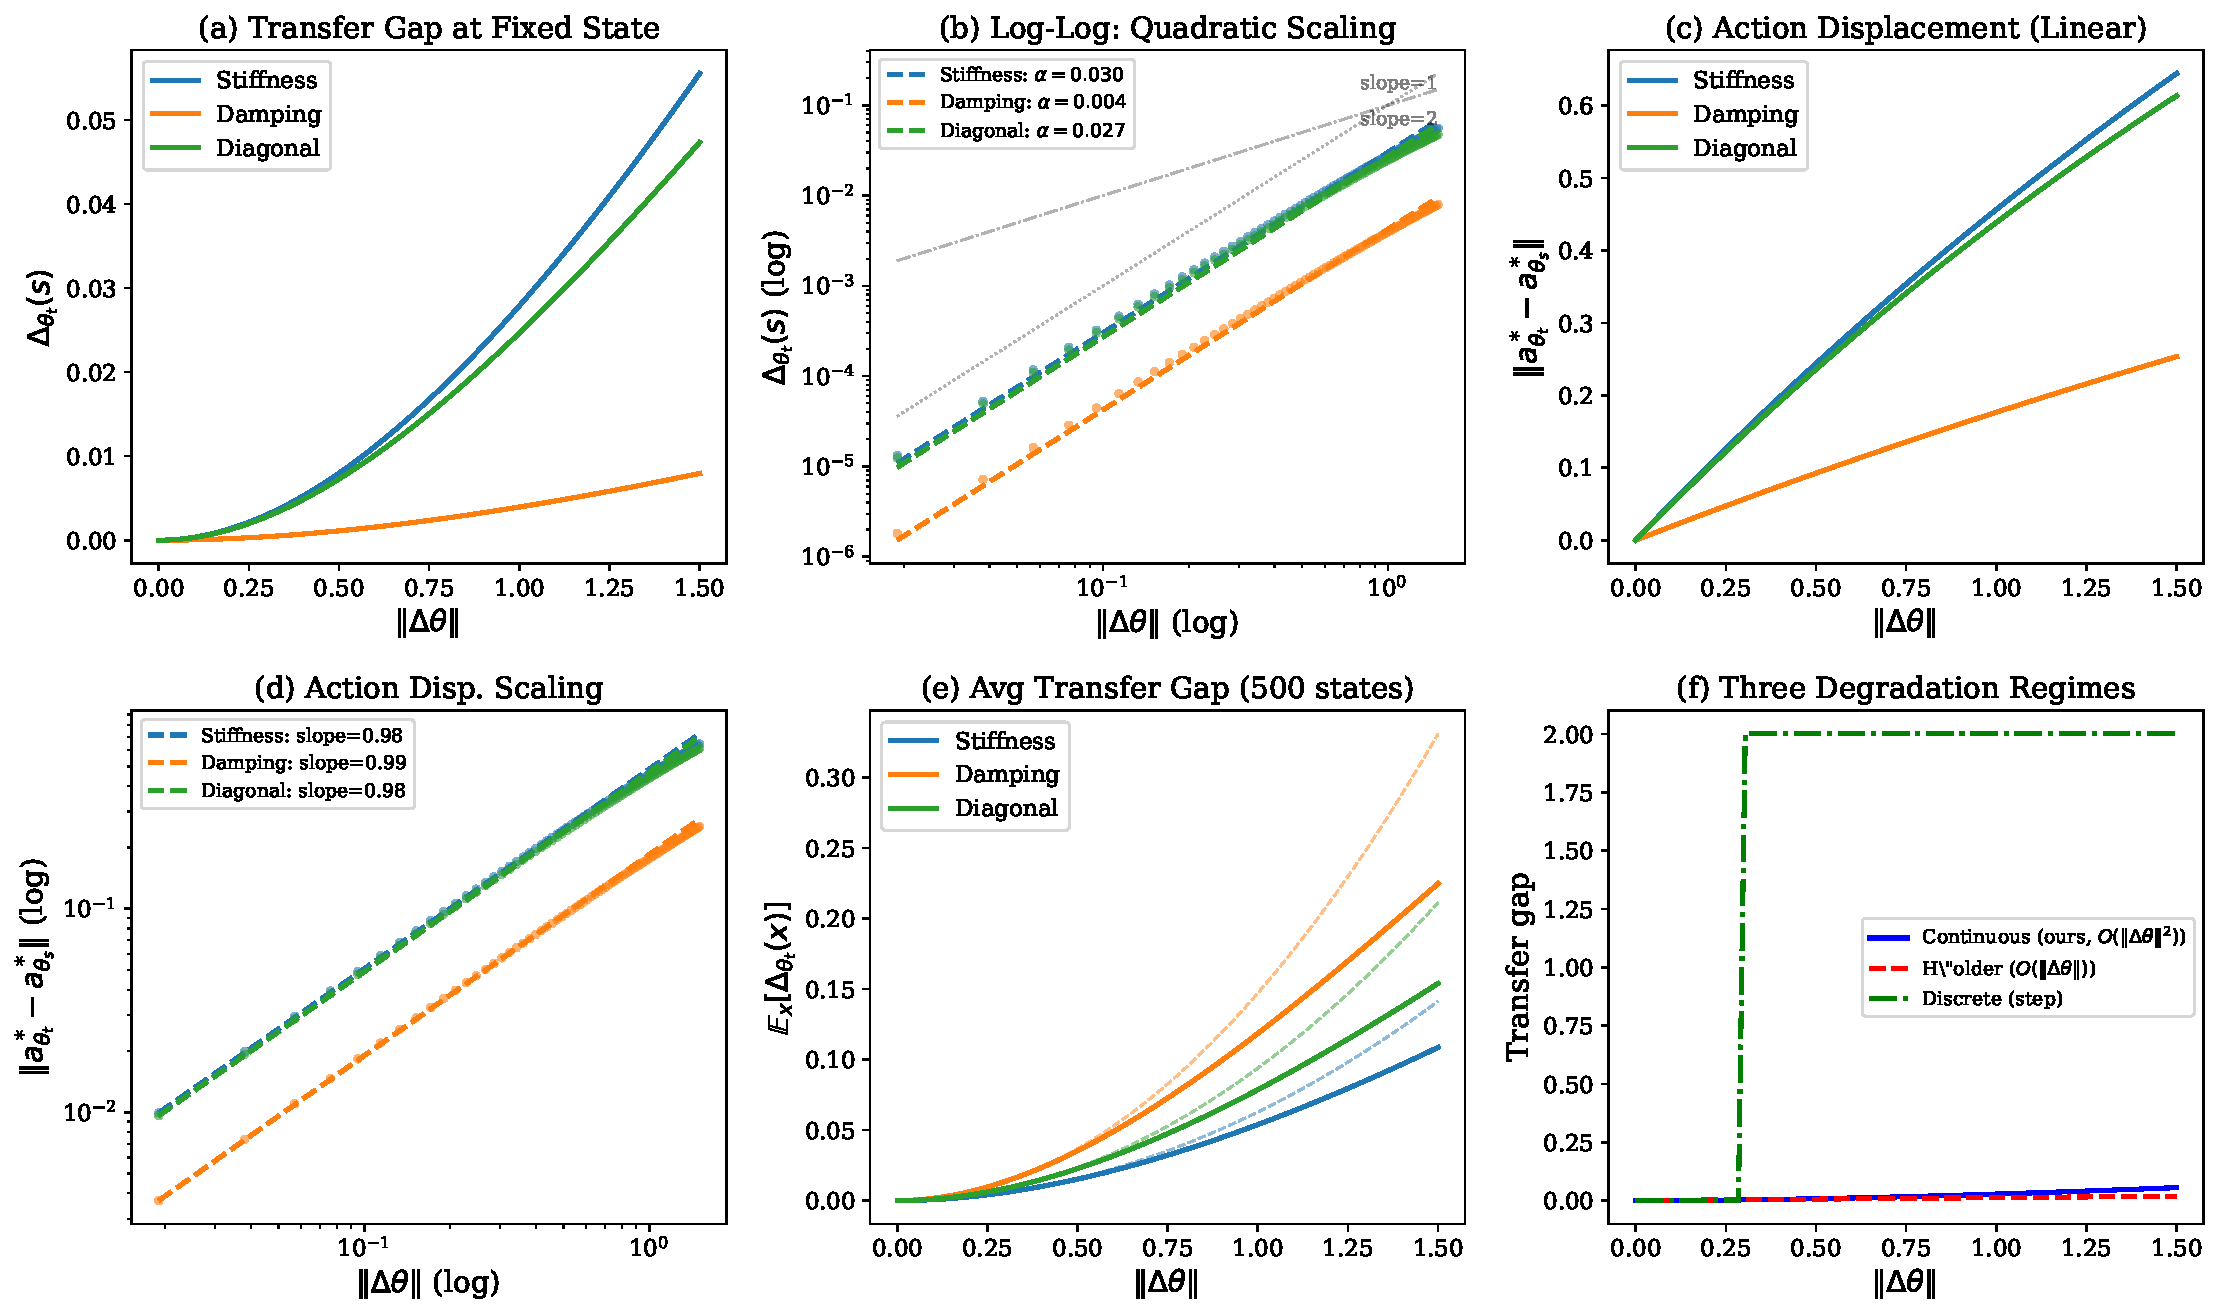
\includegraphics[width=\textwidth]{figures/exp3_lqr_quadratic.pdf}
\caption{LQR quadratic degradation. (a) Transfer gap. (b) Log-log confirms slope 2. (c)--(d) Action displacement is linear. (e) Average over 500 states. (f) Three degradation regimes.}
\label{fig:lqr}
\end{figure}

\subsection{Control Environment Transfer}
\label{app:exp-gymnasium}

\paragraph{Setup.} Two control environments: Wind Grid (discrete, $6 \times 6$ grid, 4 actions, $\theta =$ wind strength) with a goal at the corner and wind pushing the agent away, and Pendulum (continuous, $\theta =$ gravity) using analytical LQR with Lyapunov-based transfer gap computation. No simulation noise; all pendulum results are fully analytical.

\paragraph{Results.} Wind Grid (Figure~\ref{fig:gymnasium}(a)): the source policy degrades smoothly as wind strength increases. Ordinal consistency declines gradually from $1.0$ to $0.6$ (Figure~\ref{fig:gymnasium}(b)) and the number of violation states $|\Sviol|$ grows from $0$ to $14$ out of $36$ (Figure~\ref{fig:gymnasium}(c)). This gradual pattern (rather than sudden failure) shows that ordinal structure erodes state by state as the perturbation grows. The Pendulum (Figure~\ref{fig:gymnasium}(d)--(e)) confirms our continuous-action theory: the transfer gap grows quadratically with $|\Delta g|$ (log-log slope $\approx 1.9$), and the gain displacement $\|K_t - K_s\|$ is linear in $|\Delta g|$ (slope $\approx 0.93$, Figure~\ref{fig:gymnasium}(f)), consistent with Theorems~\ref{thm:quadratic-subopt}--\ref{thm:action-displacement} (Appendix~\ref{app:proofs}).

\begin{figure}[h]
\centering
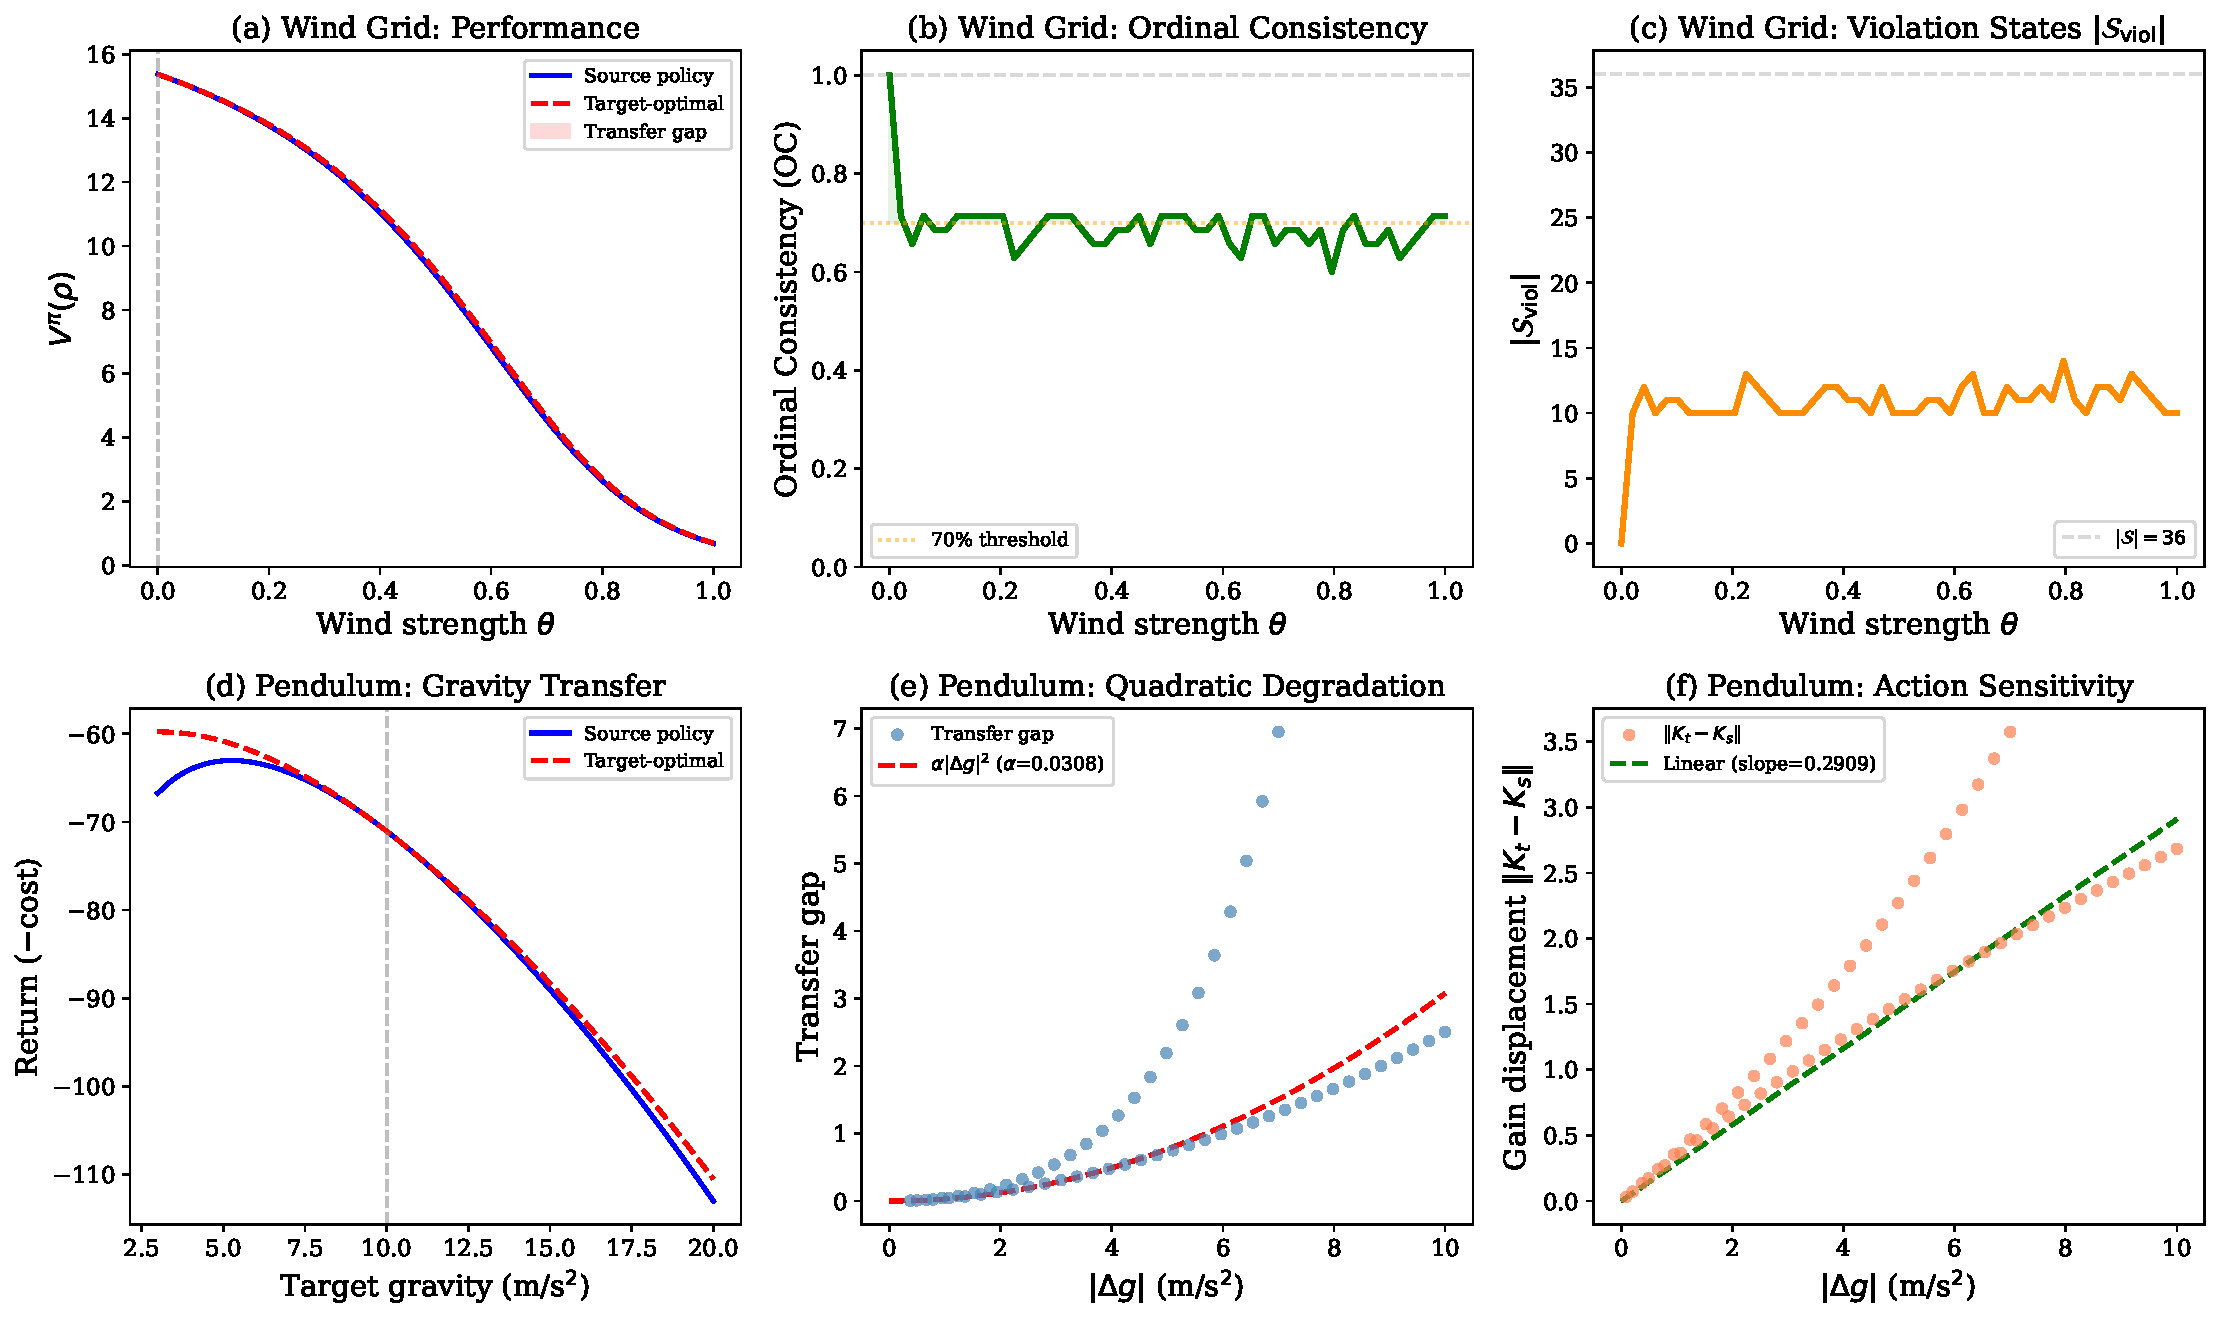
\includegraphics[width=\textwidth]{figures/exp4_gymnasium.pdf}
\caption{Control environments. Top: Wind Grid ($6 \times 6$, discrete). (a) Smooth performance degradation. (b) Gradual OC decline ($1.0 \to 0.6$). (c) $|\Sviol|$ grows to 14/36. Bottom: Pendulum (continuous, analytical LQR). (e) Quadratic degradation (slope $\approx 1.9$). (f) Linear gain displacement (slope $\approx 0.93$).}
\label{fig:gymnasium}
\end{figure}

\subsection{Sample Complexity (Theorem~\ref{thm:sample-complexity}; continuous version in \S\ref{app:proofs})}
\label{app:exp-sample}

\paragraph{Setup.} \textbf{Discrete:} 6-state, 3-action MDP with shared transitions and $\theta$-dependent rewards, where three states have orderings that flip at $\theta = 0$. Source distribution $\theta \sim \mathrm{Uniform}(-0.3, 0.7)$ creates $\sim 30\%$ minority disagreement. Majority-vote policy from $K$ i.i.d.\ sources. \textbf{Continuous:} Mean-action policy from $K$ LQR sources, evaluated over 6 test states.

\paragraph{Results.} Figure~\ref{fig:sample}(a): majority-vote accuracy increases from $0.84$ at $K = 1$ to $1.0$ at $K = 50$, with the theoretical threshold $K^* \approx 80$ (Theorem~\ref{thm:sample-complexity}, $\kappa_{\min} = 0.19$) closely matching the empirical convergence point. Figure~\ref{fig:sample}(b) validates the model-free certificate (Proposition~\ref{prop:model-free}): the estimated margin $\hat{\kappa}$ is negative for small $K$ (insufficient data) but crosses zero around $K = 100$ and converges toward the true $\kappa_{\min} = 0.19$ as $K$ increases, confirming that source policy agreement alone can certify ordinal consistency. Figure~\ref{fig:sample}(c) validates Corollary~\ref{cor:noisy-q}: accuracy stays near $1.0$ for $\epsilon_Q < g_{\min}/2 \approx 0.09$, then drops sharply. For continuous actions (Figure~\ref{fig:sample}(d)--(f)), the MSE decreases as $O(1/K)$ and the transfer gap follows the theoretical bound $\frac{L_{aa}}{2} \cdot \frac{\sigma^2}{K}$, both consistent with Theorem~\ref{thm:continuous-sample} (Appendix~\ref{app:proofs}).

\begin{figure}[h]
\centering
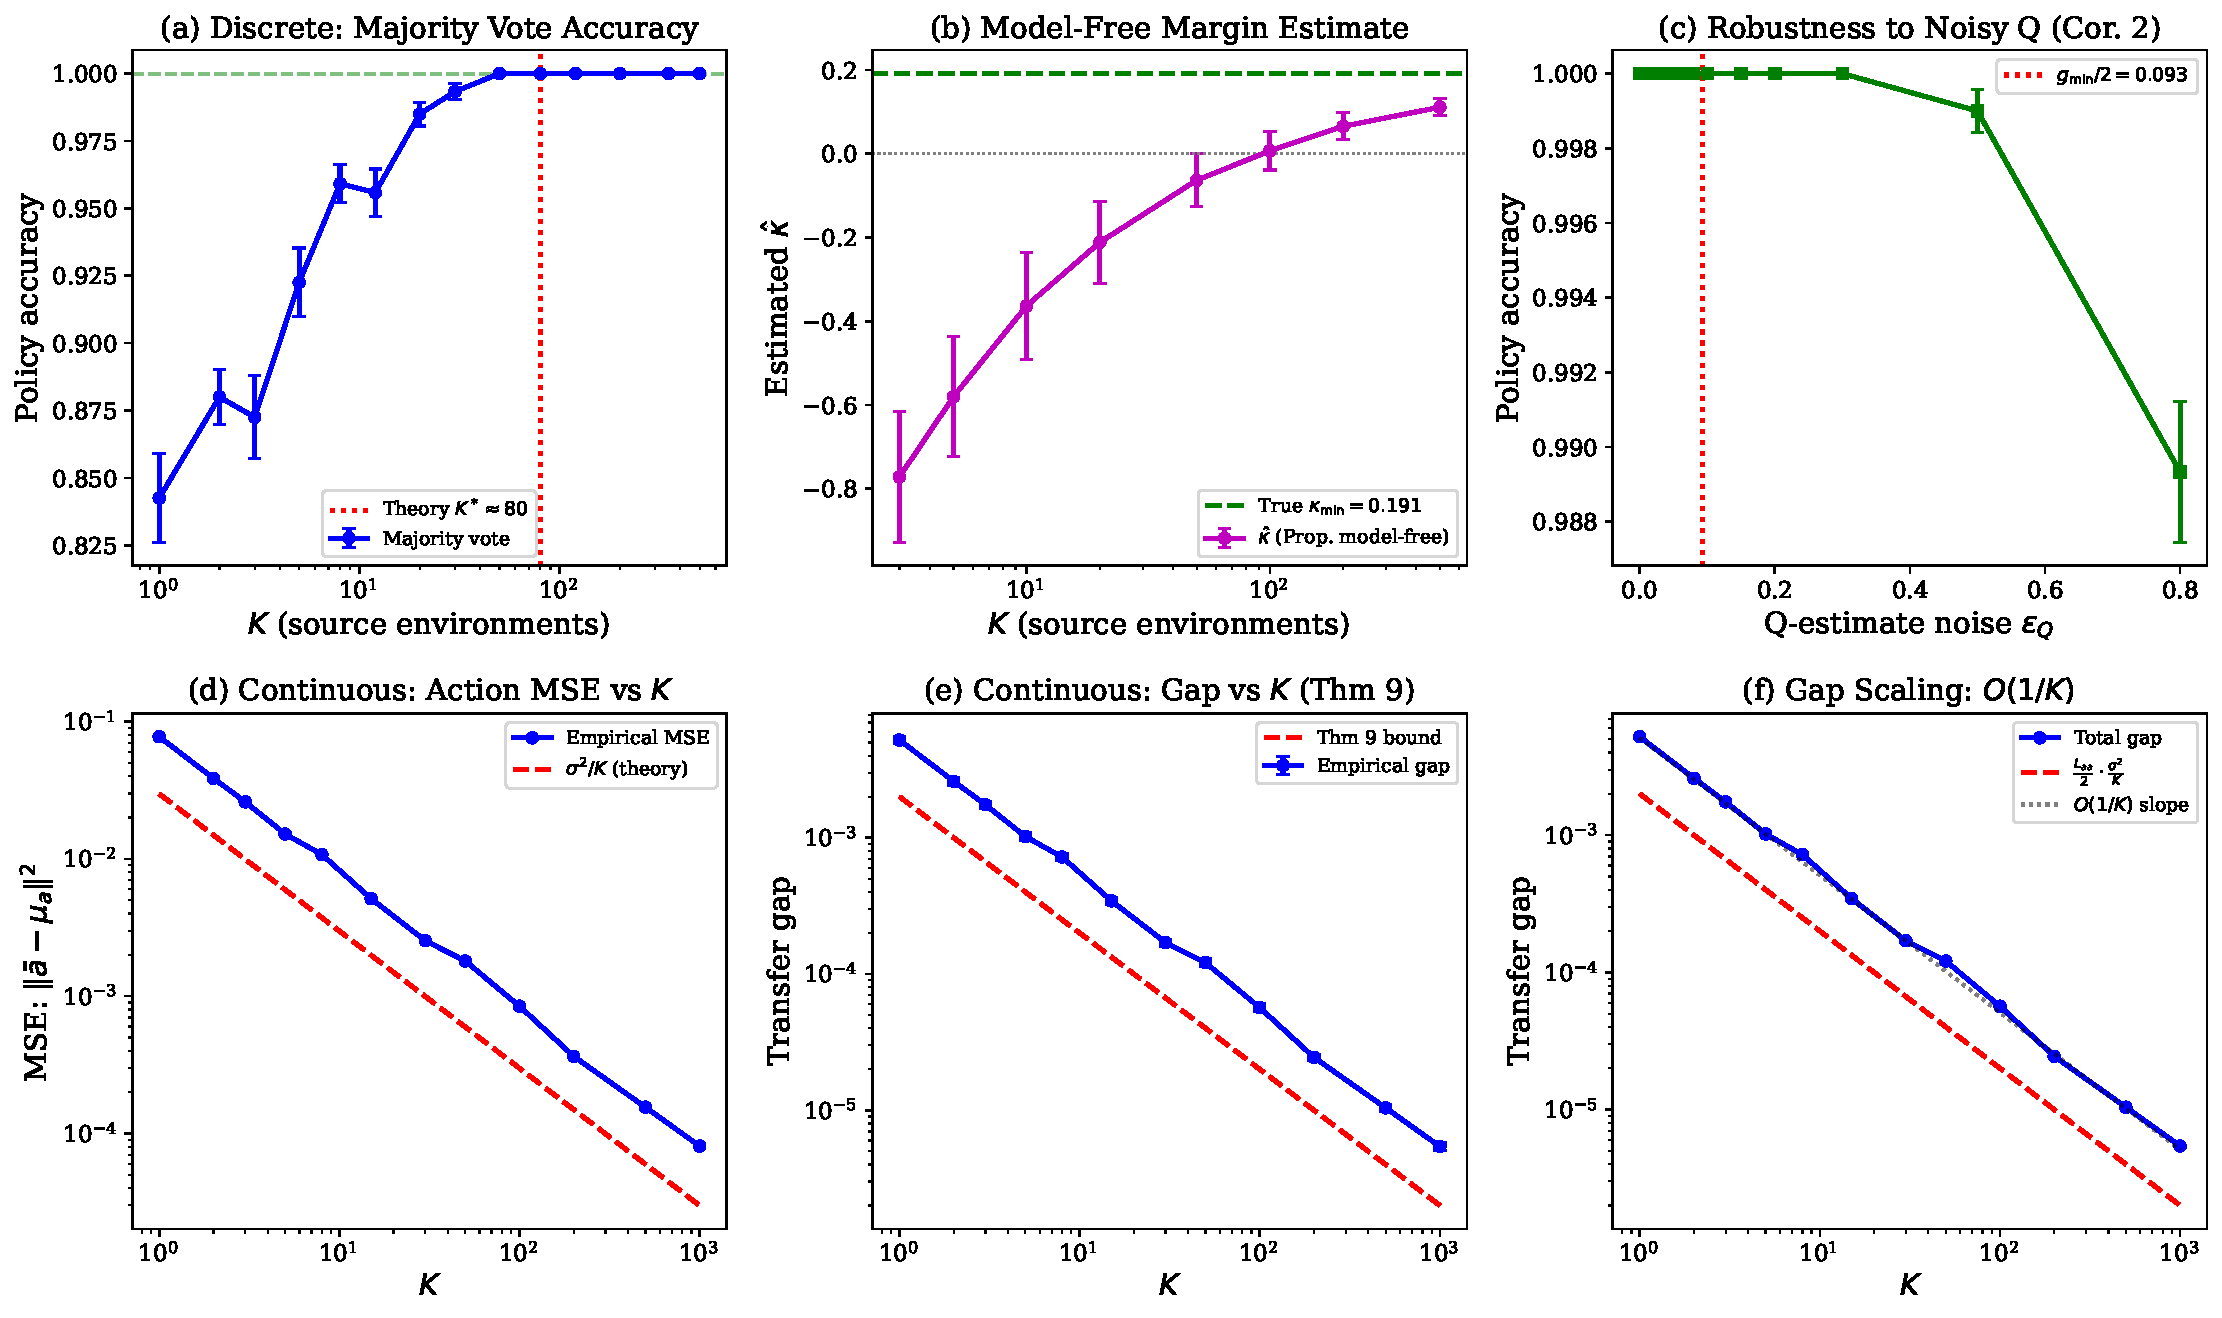
\includegraphics[width=\textwidth]{figures/exp5_sample_complexity.pdf}
\caption{Sample complexity. Top: discrete. (a) Majority-vote accuracy vs.\ $K$, with $K^* \approx 80$. (b) Model-free $\hat{\kappa}$ estimate converges to true $\kappa_{\min}$ (Prop.~\ref{prop:model-free}). (c) Noise robustness ($g_{\min}/2 \approx 0.09$). Bottom: continuous mean-action. (d) MSE $\sim O(1/K)$. (e) Gap matches the continuous-sample bound (see Appendix~\ref{app:proofs}). (f) $O(1/K)$ scaling.}
\label{fig:sample}
\end{figure}

\subsection{Higher-Dimensional Transfer (4-joint robot)}
\label{app:exp-mujoco}

\paragraph{Setup.} 4-joint robot surrogate (8-dimensional state, 4-dimensional action) modeled as a linearized multi-body system. Physics parameters $\theta \in \R^3$: gravity scale, friction scale, mass scale. Policies are LQR gains, transfer gaps computed analytically.

\paragraph{Results.} Figure~\ref{fig:mujoco}(c) shows quadratic degradation (slope $\approx 2$ on log-log) across gravity, friction, mass, and combined perturbation directions, extending Theorem~\ref{thm:quadratic-subopt} (Appendix~\ref{app:proofs}) to higher dimensions. The gain displacement (policy change) is linear (Figure~\ref{fig:mujoco}(e)), consistent with Theorem~\ref{thm:action-displacement} (Appendix~\ref{app:proofs}). The 2D heatmap (Figure~\ref{fig:mujoco}(d)) shows the transfer gap landscape is smooth and convex around the source parameter, supporting the local strong concavity assumption (Assumption~\ref{asm:local-sc}).

\begin{figure}[h]
\centering
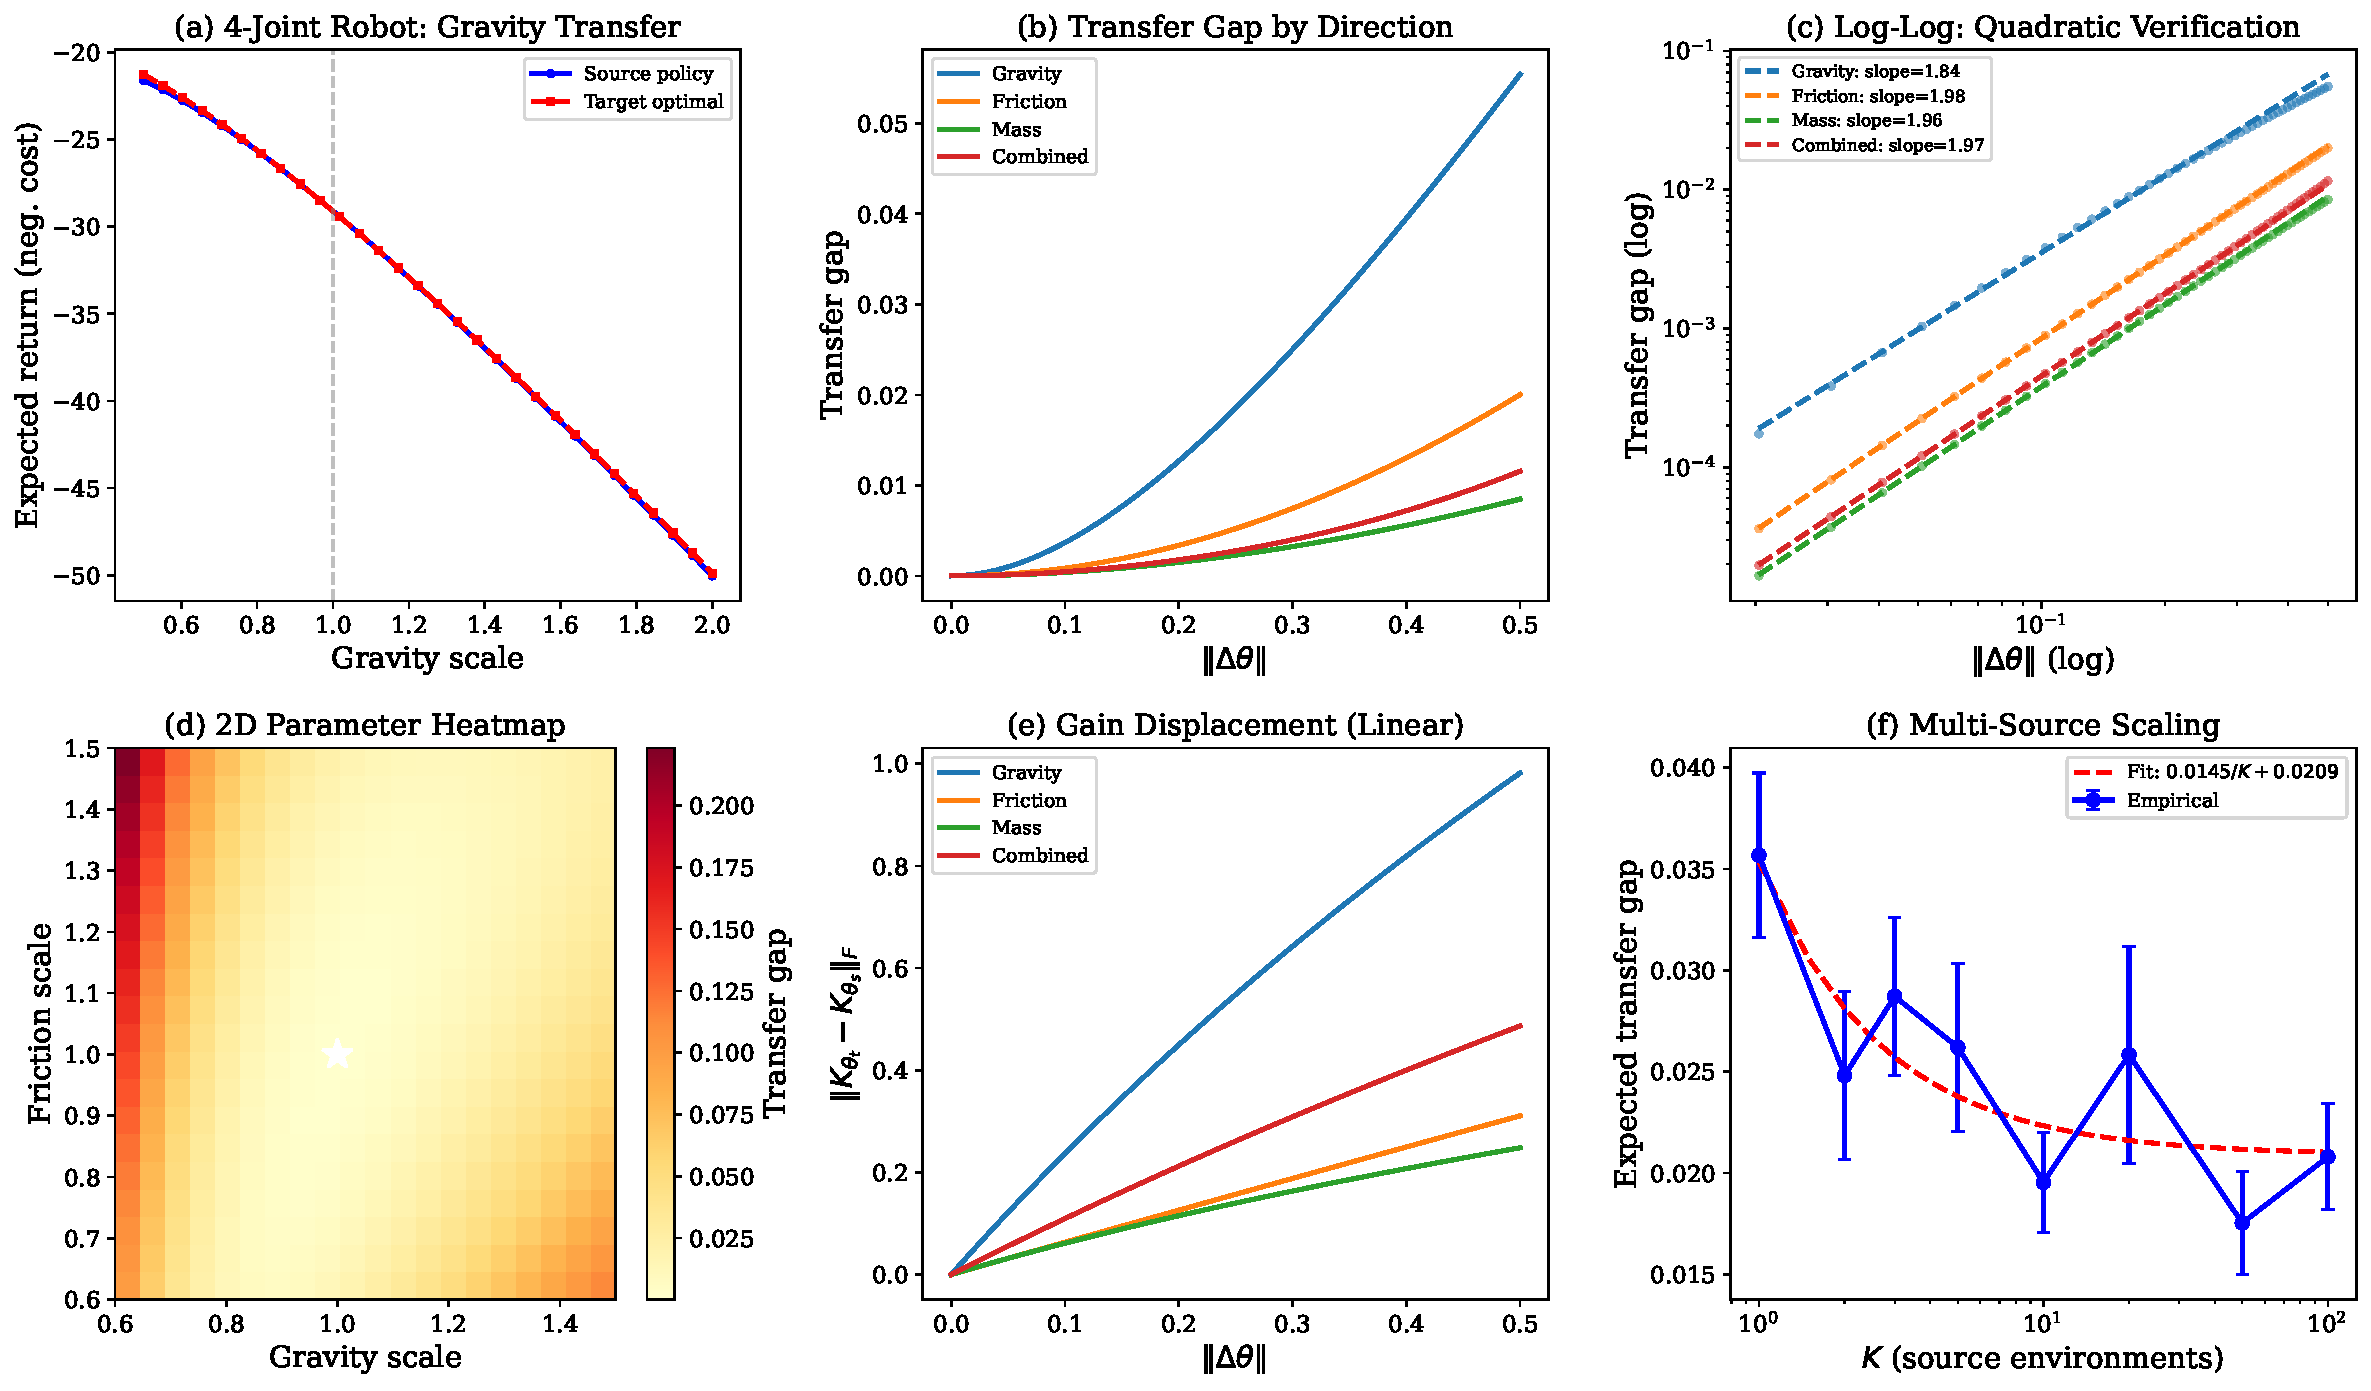
\includegraphics[width=\textwidth]{figures/exp7_mujoco.pdf}
\caption{4-joint robot surrogate. (a) Return vs.\ gravity. (b) Gap by perturbation direction. (c) Log-log: slope $\approx 2$. (d) 2D gap heatmap. (e) Linear gain displacement. (f) Multi-source scaling.}
\label{fig:mujoco}
\end{figure}

\subsection{Supplementary Figures for Main-Body Neural Experiments (\S\ref{sec:exp-neural})}
\label{app:exp-neural-figs}

\begin{figure}[h]
\centering
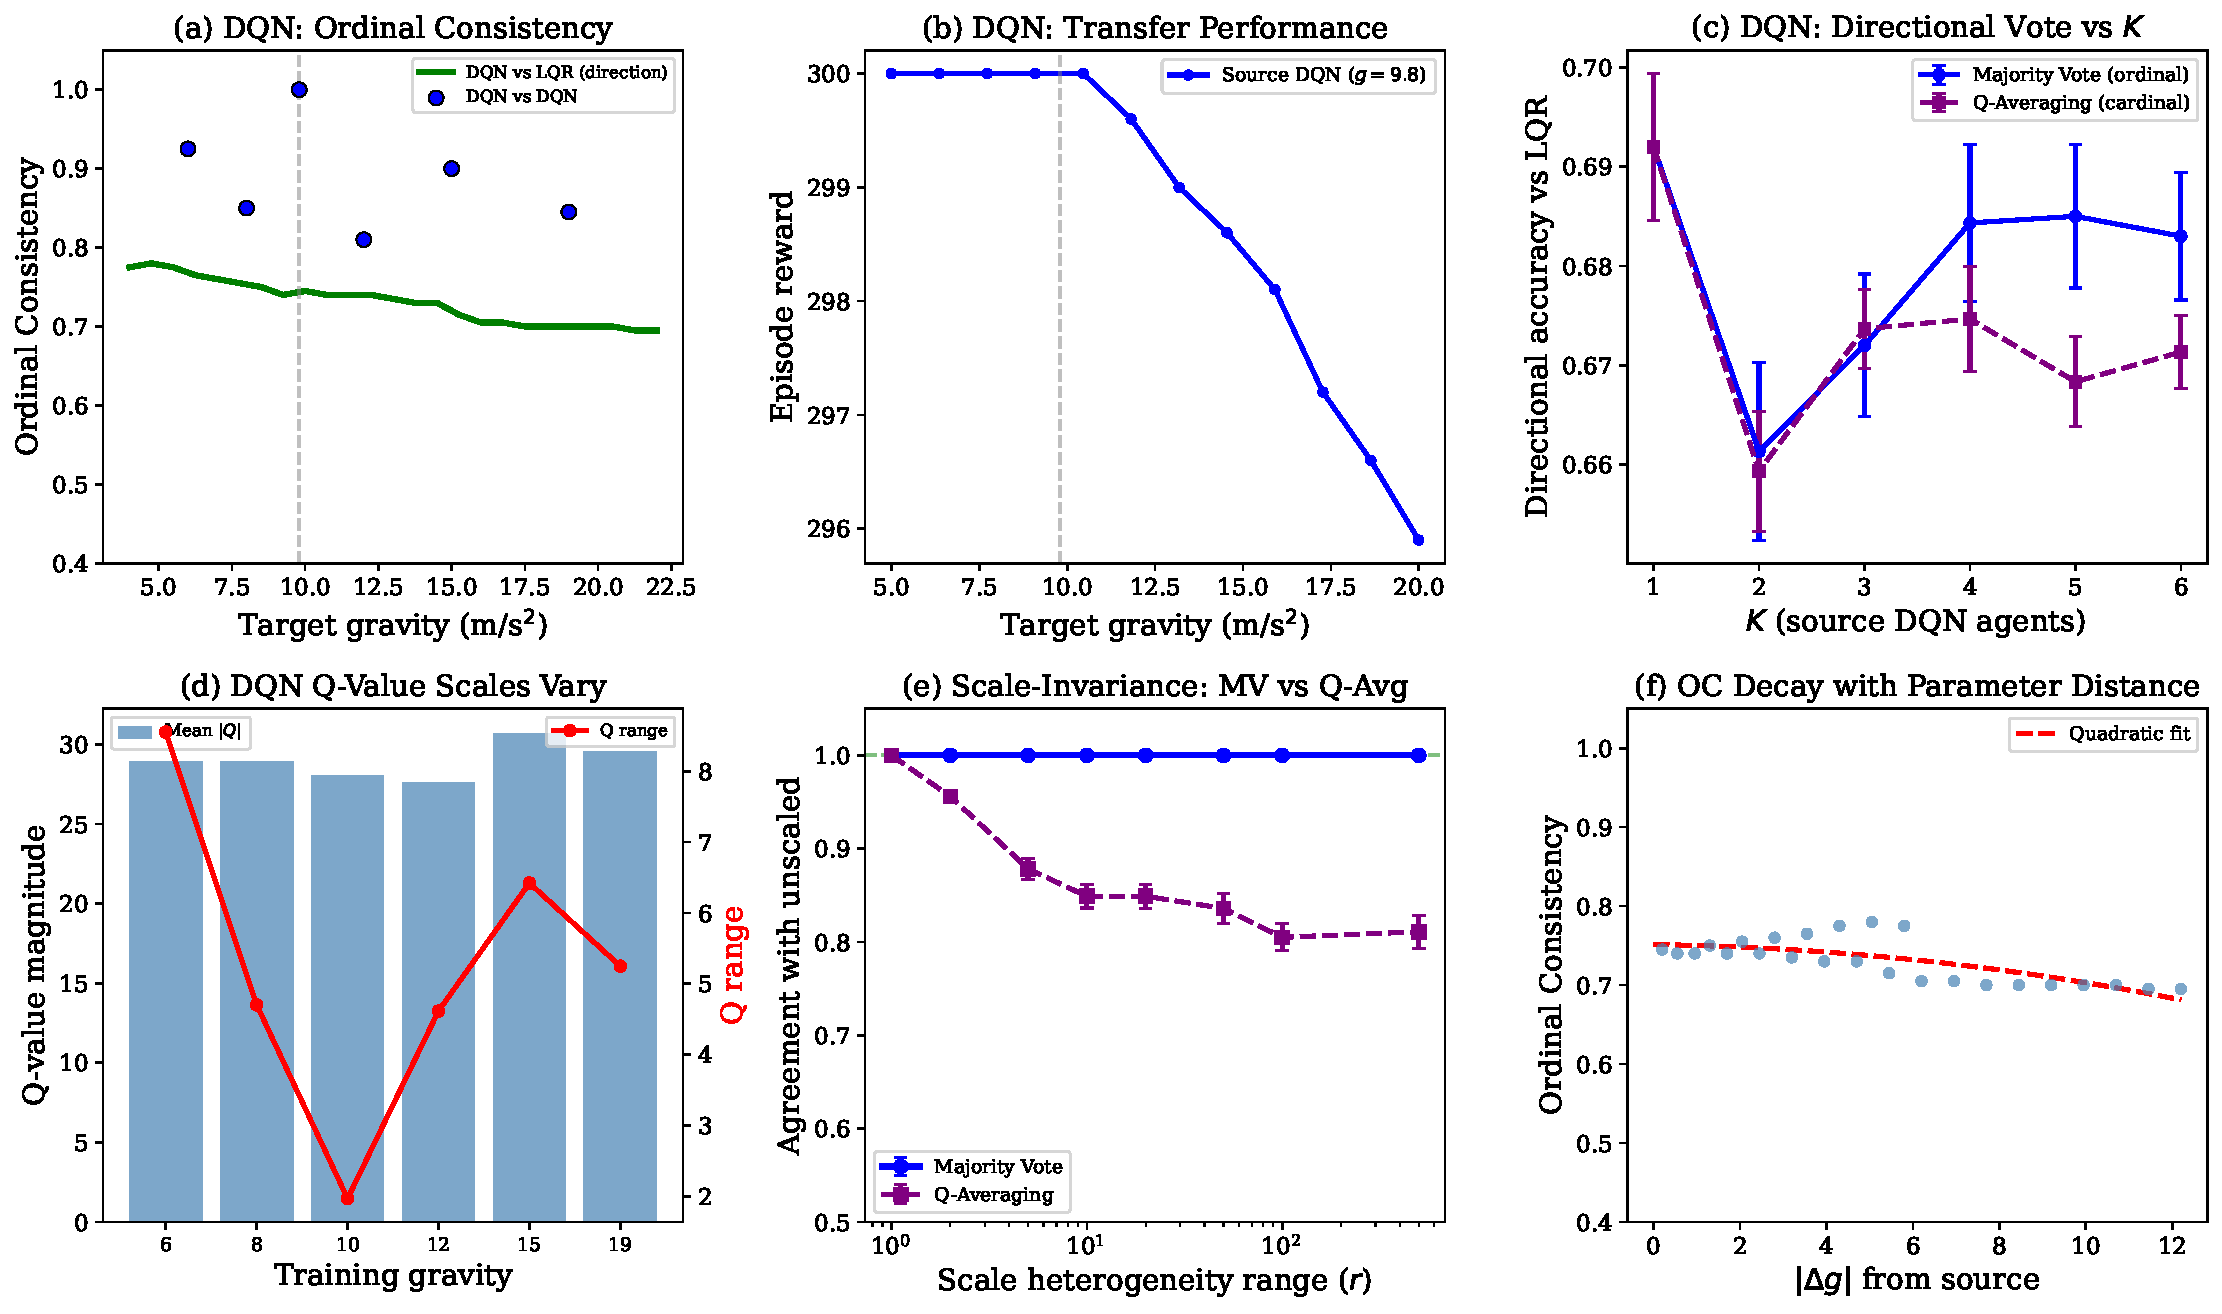
\includegraphics[width=\textwidth]{figures/exp8_dqn_transfer.pdf}
\caption{4-action CartPole with DQN. Directional OC between source DQN ($g=9.8$) and LQR-optimal decays smoothly from ${\approx}0.95$ to ${\approx}0.75$ at extreme gravities. Majority vote maintains agreement $=1.0$ at scale ranges up to $100\times$, while Q-averaging drops to $0.81$.}
\label{fig:dqn}
\end{figure}

\begin{figure}[h]
\centering
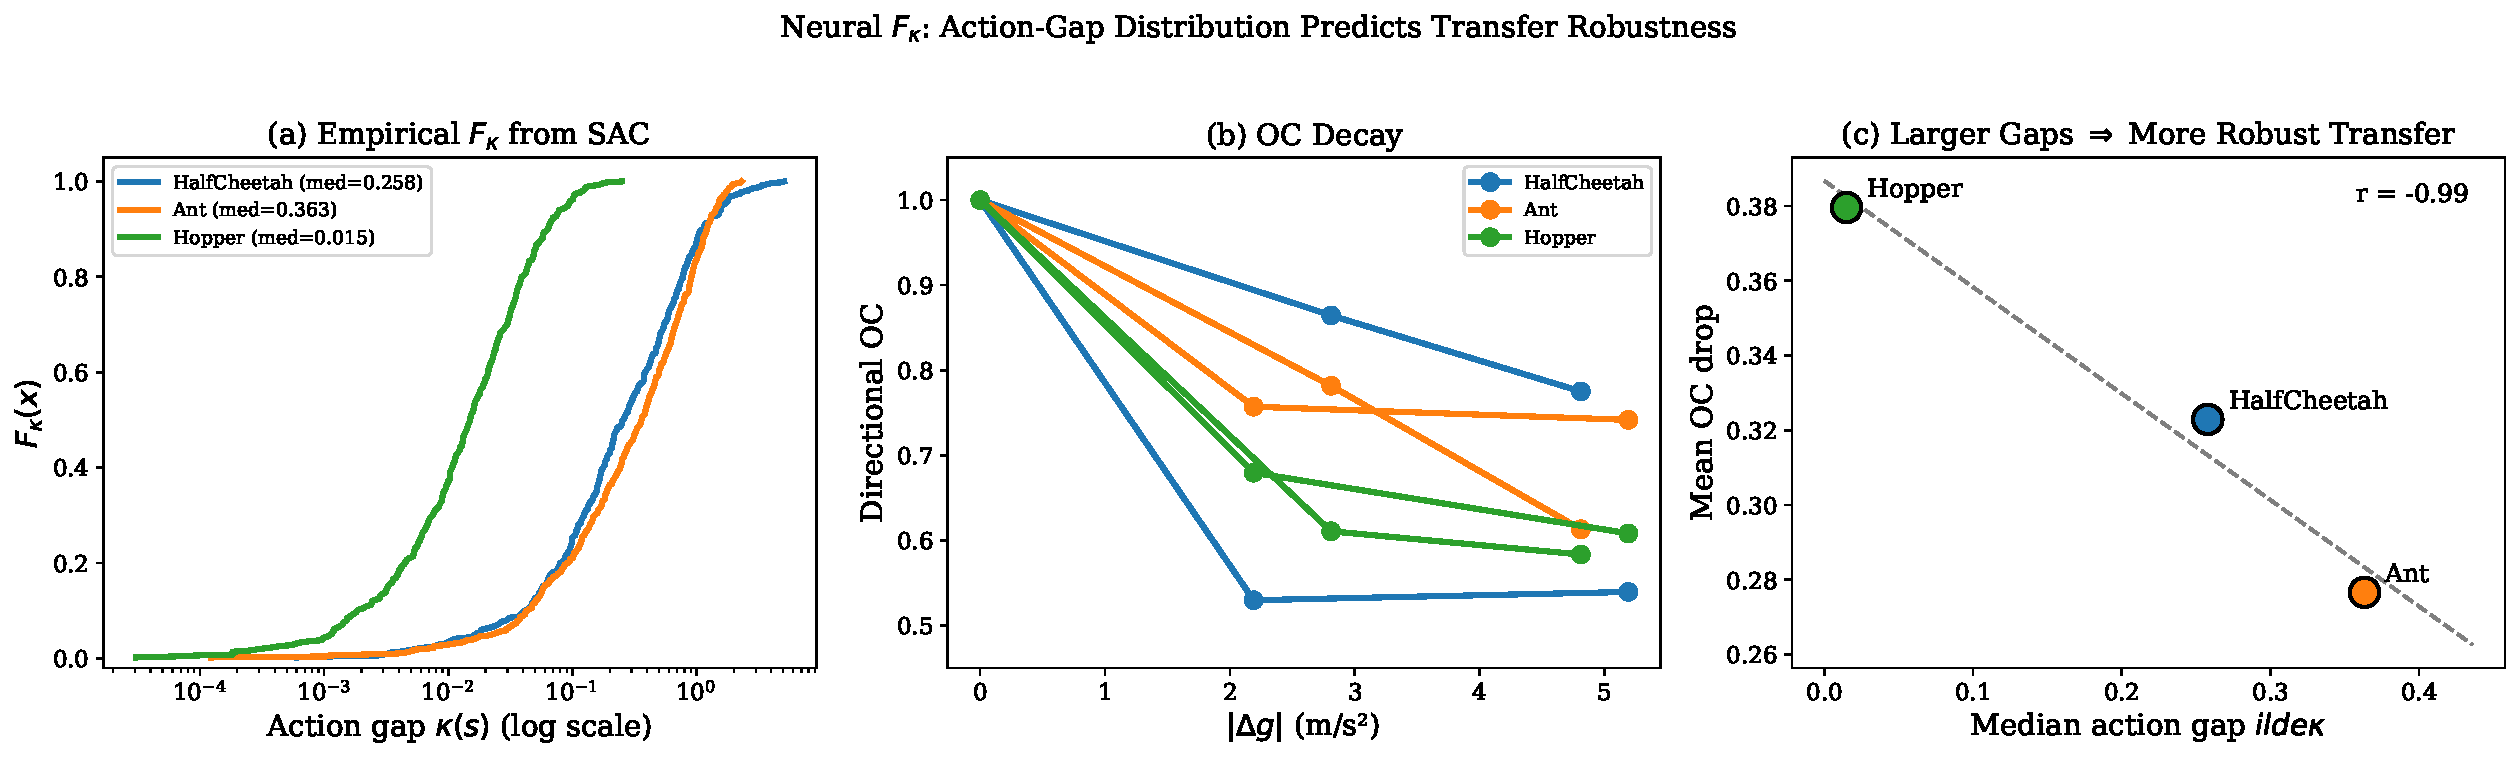
\includegraphics[width=\textwidth]{figures/exp14_fkappa_neural.pdf}
\caption{$F_\kappa$ predicts transfer robustness in neural settings. (a)~Empirical action-gap CDFs from SAC: Hopper's gaps are ${\sim}20\times$ smaller. (b)~OC decay across environments. (c)~Median gap vs.\ OC drop on three environments: the qualitative ordering matches the $F_\kappa$ framework's prediction (smaller median gap, less robust transfer); three points cannot establish a quantitative law, so we treat this panel as illustrative and defer to per-target validation in Appendix~\ref{app:fkappa-bound} (Table~\ref{tab:fkappa-bound}, $12$ tests).}
\label{fig:fkappa-neural}
\end{figure}

\subsection{Multi-Seed SAC Results (full table and curves)}
\label{app:multiseed}

\begin{figure}[h]
\centering
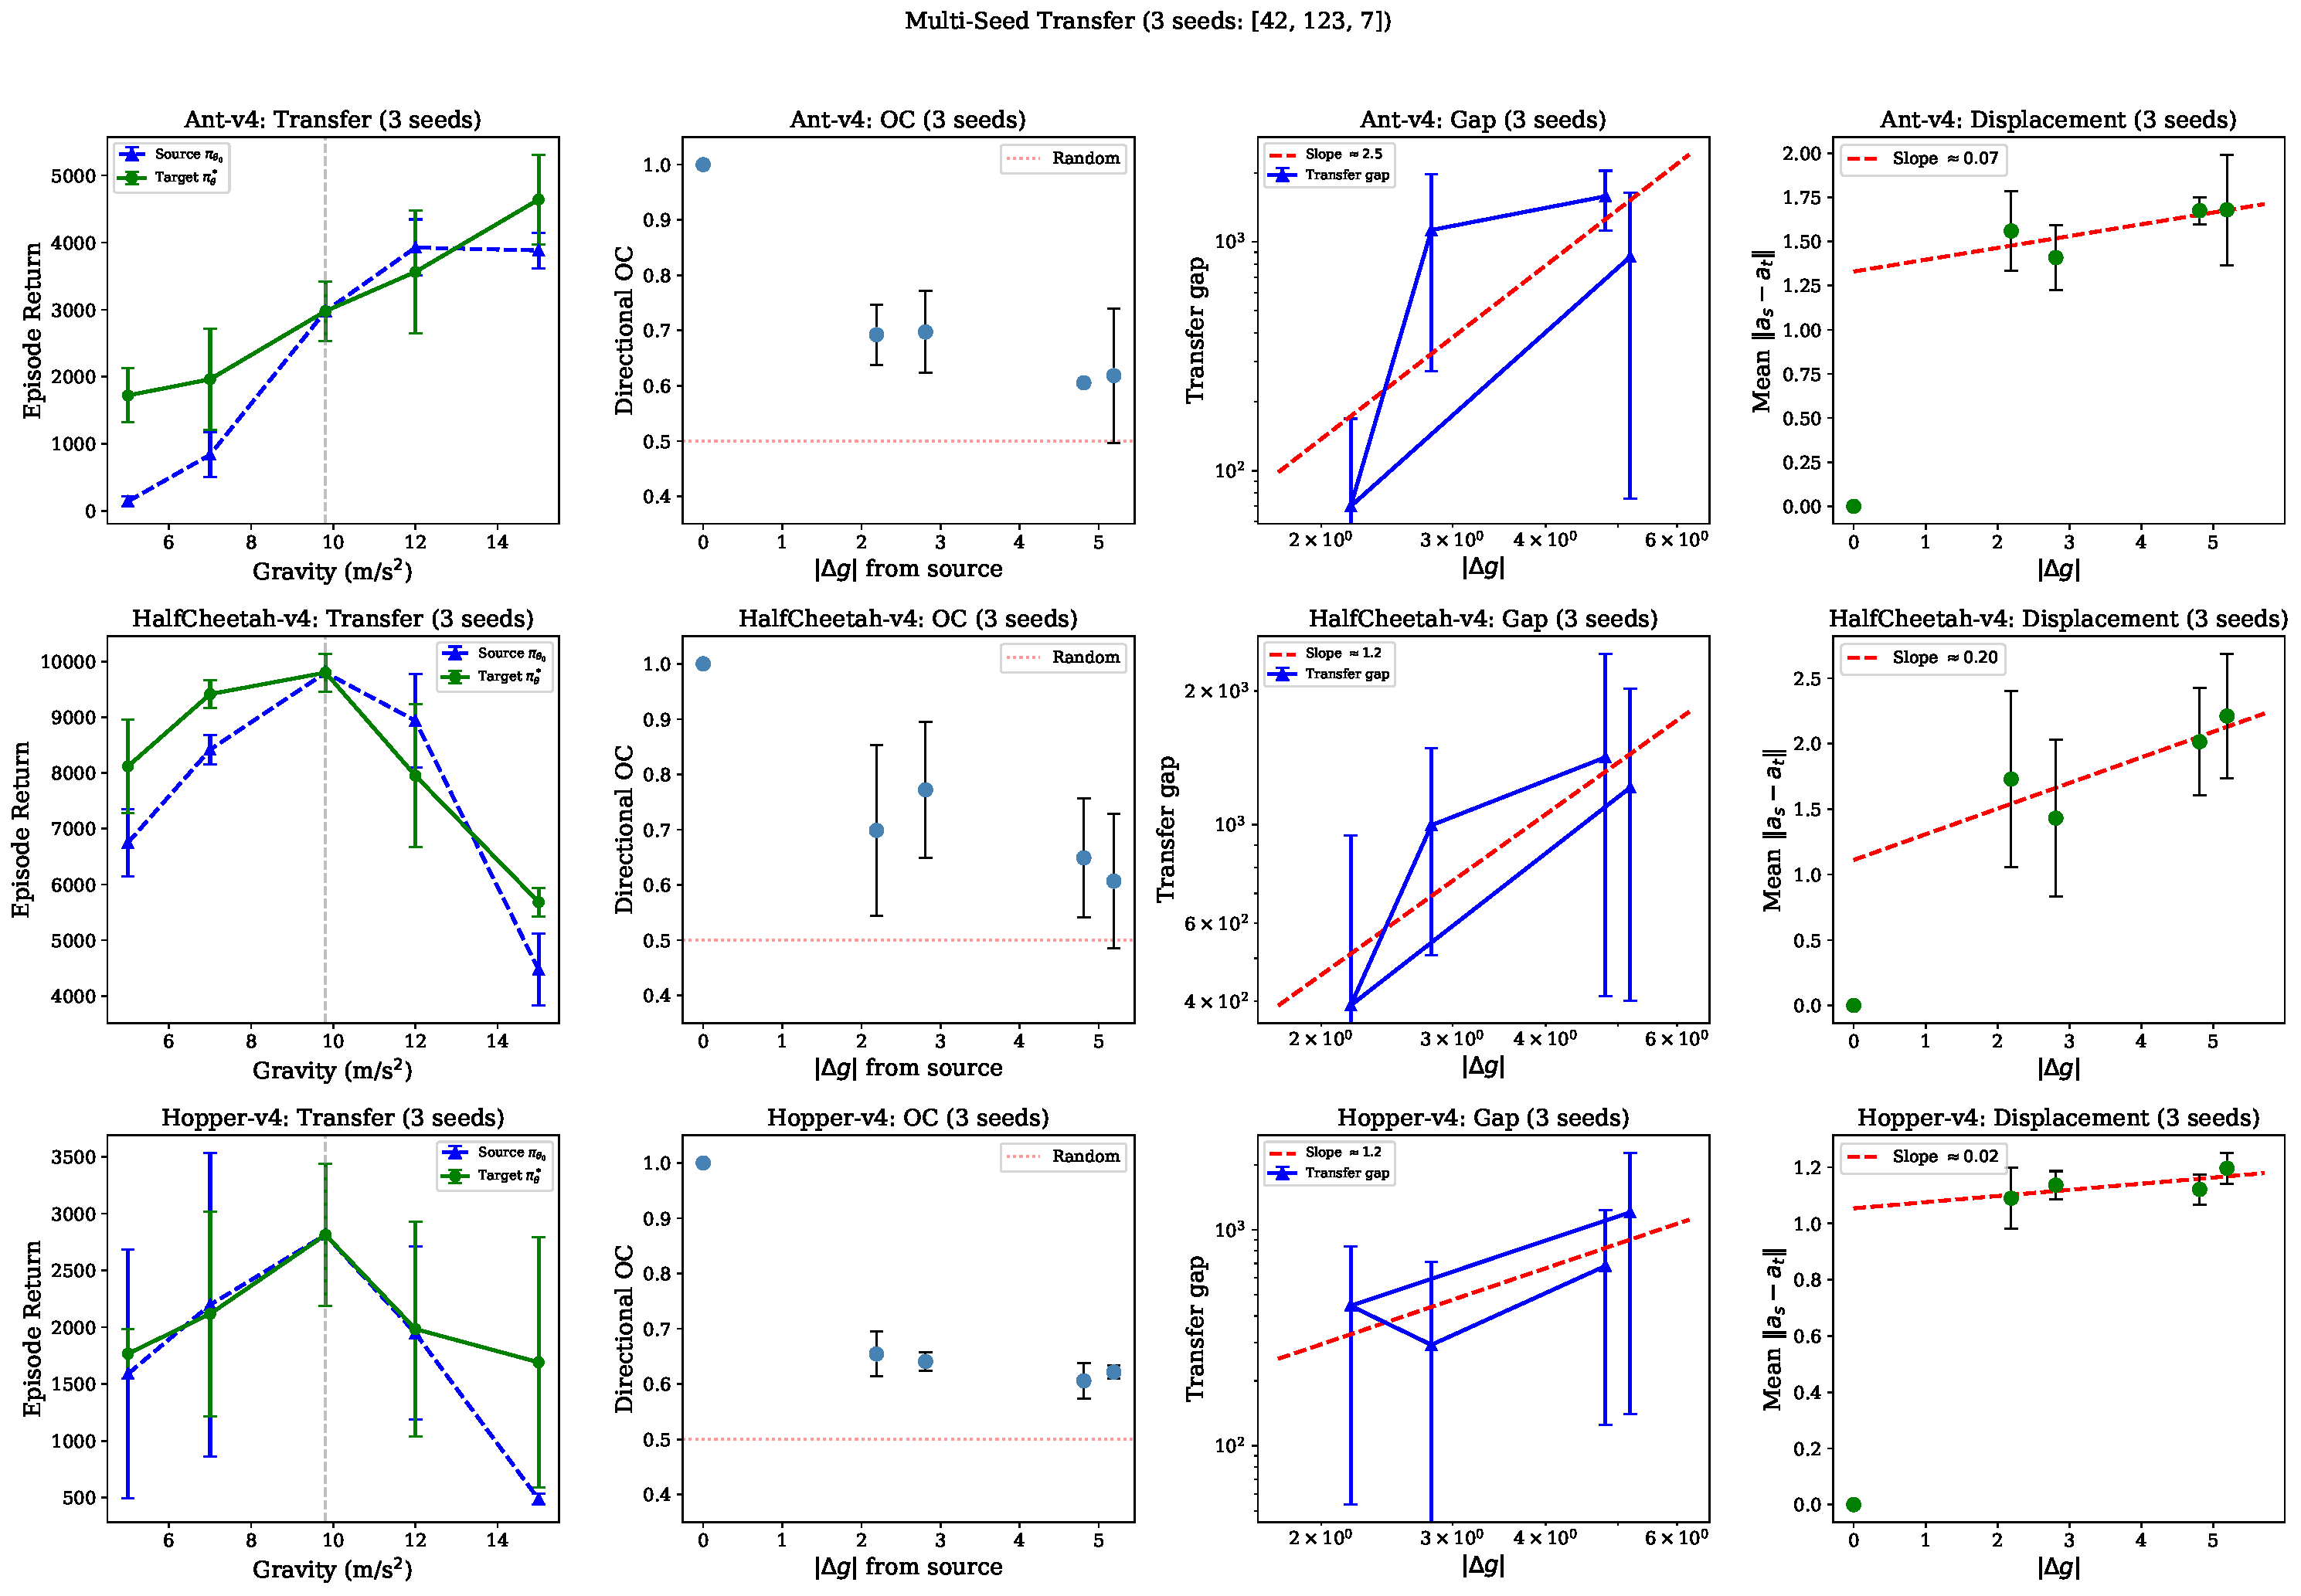
\includegraphics[width=\textwidth]{figures/exp10_multiseed.pdf}
\caption{Multi-seed transfer across three MuJoCo environments (3 seeds; error bars show $\pm 1$ std). Rows: Ant, HalfCheetah, Hopper. Columns: (a) Transfer return. (b) Directional OC. (c) Transfer gap (log-log). (d) Action displacement. OC decay is consistent across seeds in every environment (std $\leq 0.15$); gap magnitudes carry larger variance, so we interpret qualitative trends rather than specific values.}
\label{fig:multiseed}
\end{figure}

\begin{table}[h]
\centering
\caption{Log-log transfer-gap slopes under identical fit protocol (gap clipped at $1$, $|\Delta g| > 0.3$). Single-seed fits use 11 gravities ($\{5,6,\ldots,15\}$); multi-seed avg fits the mean gap across seeds $\{42,123,7\}$ on $5$ gravities ($\{5,7,9.81,12,15\}$). Aggregated slopes are more modest because averaging smooths seed-specific extremes; the qualitative fragility ordering (Hopper $\lesssim$ HalfCheetah $\leq$ Ant) is preserved.}
\label{tab:slope-comparison}
\small
\begin{tabular}{lcc}
\toprule
Env & Single-seed slope (Fig.~\ref{fig:mujoco-transfer}, seed 42) & Multi-seed avg slope (Fig.~\ref{fig:multiseed}) \\
\midrule
HalfCheetah & $4.56$ & $1.20$ \\
Ant         & $4.19$ & $2.52$ \\
Hopper      & $1.88$ & $1.17$ \\
\bottomrule
\end{tabular}
\end{table}

\begin{table}[h]
\centering
\caption{Multi-seed SAC results on HalfCheetah-v4, Ant-v4, and Hopper-v4 (mean $\pm$ std over seeds $\{42,123,7\}$).}
\label{tab:multiseed}
\small
\begin{tabular}{llcccc}
\toprule
Env & Gravity & Source Return & Target Return & Directional OC & Action Disp. \\
\midrule
HalfCheetah & 5.0  & $6{,}748 \pm 608$  & $8{,}119 \pm 845$  & $0.649 \pm 0.108$ & $2.015 \pm 0.411$ \\
            & 7.0  & $8{,}417 \pm 259$  & $9{,}414 \pm 243$  & $0.772 \pm 0.123$ & $1.432 \pm 0.599$ \\
            & 9.81 & $9{,}799 \pm 338$  & $9{,}799 \pm 338$  & $1.000 \pm 0.000$ & $0.000 \pm 0.000$ \\
            & 12.0 & $8{,}936 \pm 843$  & $7{,}950 \pm 1283$ & $0.699 \pm 0.154$ & $1.729 \pm 0.672$ \\
            & 15.0 & $4{,}472 \pm 642$  & $5{,}684 \pm 257$  & $0.607 \pm 0.122$ & $2.212 \pm 0.476$ \\
\midrule
Ant         & 5.0  & $143 \pm 72$       & $1{,}723 \pm 404$  & $0.605 \pm 0.003$ & $1.675 \pm 0.076$ \\
            & 7.0  & $839 \pm 332$      & $1{,}963 \pm 751$  & $0.697 \pm 0.074$ & $1.409 \pm 0.182$ \\
            & 9.81 & $2{,}978 \pm 443$  & $2{,}978 \pm 443$  & $1.000 \pm 0.000$ & $0.000 \pm 0.000$ \\
            & 12.0 & $3{,}926 \pm 420$  & $3{,}563 \pm 919$  & $0.692 \pm 0.055$ & $1.560 \pm 0.225$ \\
            & 15.0 & $3{,}883 \pm 263$  & $4{,}642 \pm 669$  & $0.618 \pm 0.121$ & $1.679 \pm 0.313$ \\
\midrule
Hopper      & 5.0  & $1{,}589 \pm 1094$ & $1{,}767 \pm 216$  & $0.606 \pm 0.032$ & $1.121 \pm 0.053$ \\
            & 7.0  & $2{,}198 \pm 1337$ & $2{,}118 \pm 900$  & $0.641 \pm 0.017$ & $1.137 \pm 0.050$ \\
            & 9.81 & $2{,}814 \pm 627$  & $2{,}814 \pm 627$  & $1.000 \pm 0.000$ & $0.000 \pm 0.000$ \\
            & 12.0 & $1{,}948 \pm 761$  & $1{,}984 \pm 944$  & $0.654 \pm 0.041$ & $1.090 \pm 0.109$ \\
            & 15.0 & $486 \pm 48$       & $1{,}692 \pm 1103$ & $0.622 \pm 0.012$ & $1.196 \pm 0.055$ \\
\bottomrule
\end{tabular}
\end{table}

\paragraph{Note on Ant at $g{=}5$.} The Ant source policy returns $143 \pm 72$ at $g{=}5$ versus the target-trained $1{,}723 \pm 404$, a ${\sim}12\times$ gap with an order-of-magnitude variance asymmetry. Inspection of rollouts shows the source policy frequently loses postural stability within the first ${\sim}50$ steps at this gravity (the gait learned at $g{=}9.81$ does not produce enough vertical impulse to prevent torso contact under the lighter dynamics), so the policy is not so much ``transferring poorly'' as failing to remain a coherent locomotion controller in this regime. This is consistent with the directional precondition failure documented in Appendix~\ref{app:hessian-diag}: the lighter side of Ant is precisely where the local quadratic model collapses, and the gap measured at $g{=}5$ should be read as ``regime exit,'' not as a smooth-degradation data point. The reported slope ($2.52$) is robust to this datum (excluding $g{=}5$ leaves the qualitative ordering unchanged); we keep it in the table for transparency.

\subsection{Source-Side $L_Q$ Estimator (Proposition~\ref{prop:lq-estimator})}
\label{app:exp-lq}

We validate the certified estimator $\hat L_Q^{\mathrm{cert}}$ on the same SAC ensembles trained for \S\ref{sec:exp-mujoco-transfer}. For each environment we evaluate the twin-Q minimum on $N{=}300$ on-policy states from the source gravity, sweeping the parameter ensemble $\theta_k \in \{5, 7, 9.81, 12, 15\}$ (so $K{=}5$, $h_{\max}{=}3.00$). Critic-error bound $\varepsilon_Q{=}1.0$; $H_Q$ is set to the maximum uneven-spacing second-order finite difference observed on the ensemble. This is a data-driven proxy (formally a lower bound on the true $H_Q$, since the FD samples the second derivative only at finitely many points); a safety-critical deployment would supply an a~priori $H_Q$ from physics or value-function smoothness analysis. Table~\ref{tab:lq-estimator} reports the headline numbers.

\begin{table}[h]
\centering
\caption{Source-side certified $L_Q$ on MuJoCo SAC ensembles ($N{=}300$ states, $K{=}5$ gravities). $L_Q^{\mathrm{fd}}$ is the raw first-order finite difference; $H_Q^{\mathrm{LB}}$ is the data-driven lower bound on the second-order FD; $\hat L_Q^{\mathrm{cert}}$ adds the safety-inflation terms $2\varepsilon_Q/h_k + H_Q h_k$ from Proposition~\ref{prop:lq-estimator}.}
\label{tab:lq-estimator}
\small
\begin{tabular}{lcccc}
\toprule
Env & $L_Q^{\mathrm{fd}}$ & $H_Q^{\mathrm{LB}}$ & $\hat L_Q^{\mathrm{cert}}$ & $h_{\max}$ \\
\midrule
HalfCheetah-v4 & $147.16$ & $65.22$ & $290.90$ & $3.00$ \\
Ant-v4         & $98.17$  & $45.58$ & $190.33$ & $3.00$ \\
Hopper-v4      & $34.79$  & $28.45$ & $114.28$ & $3.00$ \\
\bottomrule
\end{tabular}
\end{table}

\begin{figure}[h]
\centering
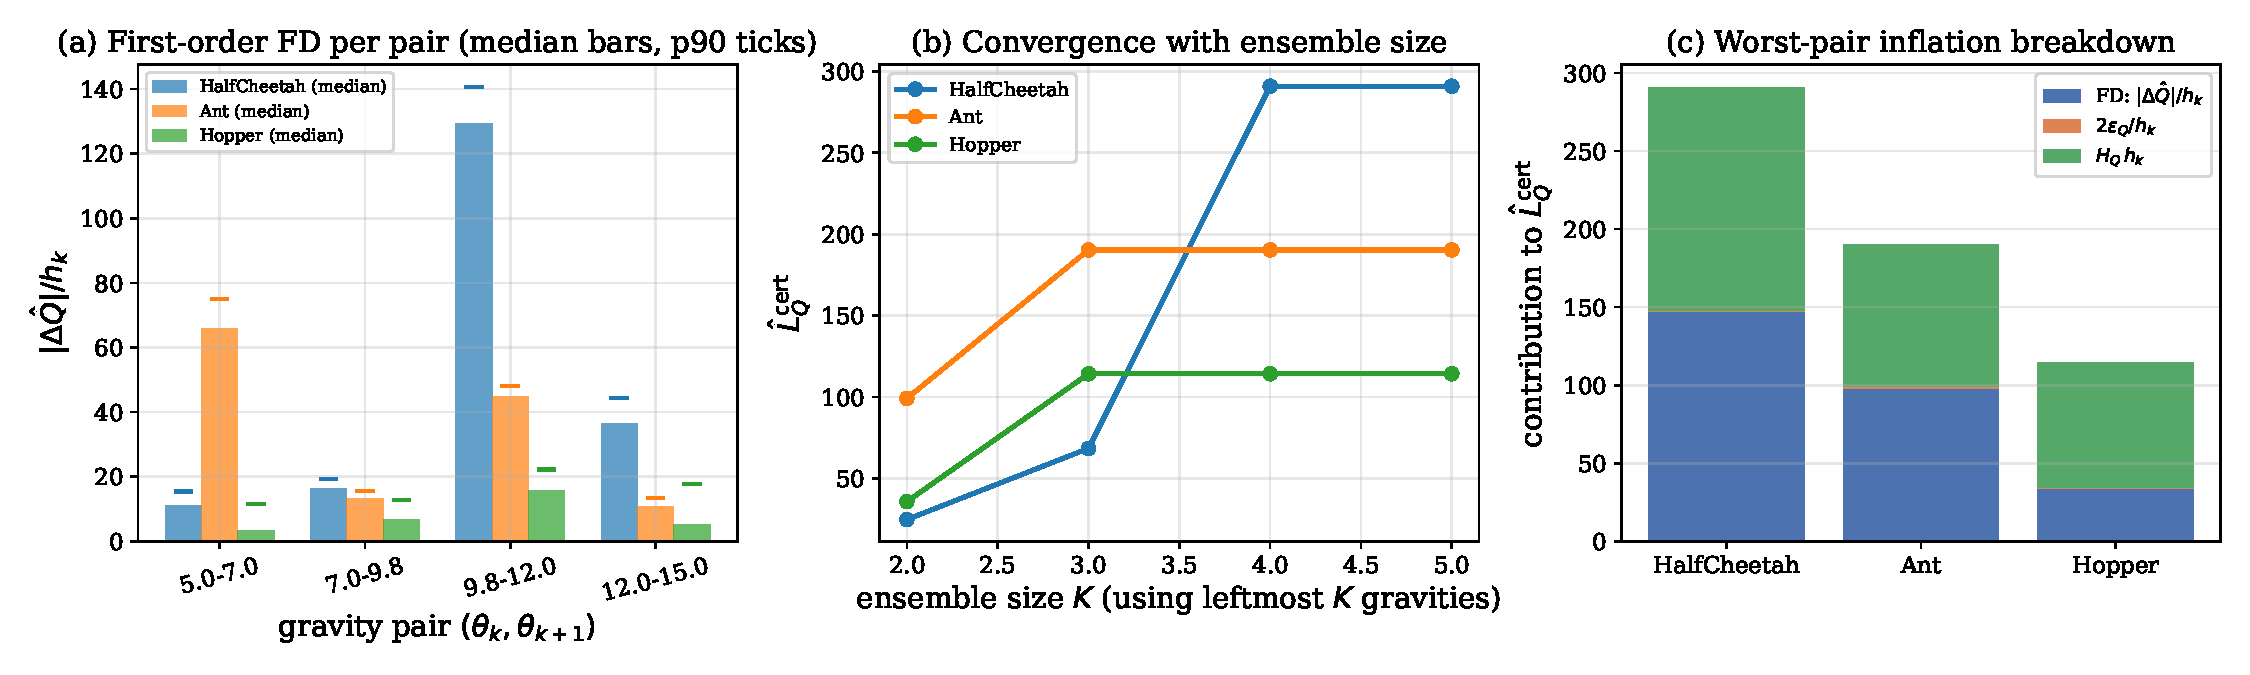
\includegraphics[width=\textwidth]{figures/exp18_lq_estimator.pdf}
\caption{Source-side $L_Q$ estimator (Proposition~\ref{prop:lq-estimator}). (a)~First-order FD per consecutive gravity pair (medians as bars; p90 ticks); HalfCheetah peaks at the $9.81$--$12.0$ pair, Ant at $5.0$--$7.0$, Hopper stays uniformly small. (b)~$\hat L_Q^{\mathrm{cert}}$ vs.\ ensemble size $K$ (using leftmost $K$ gravities); estimates plateau by $K{=}4$. (c)~Worst-pair inflation breakdown: the $H_Q h_k$ term contributes $40$--$70\%$ of the certificate (denser sampling would shrink it), while $2\varepsilon_Q/h_k$ is negligible at this $h$. Ordering ($\mathrm{Hopper} < \mathrm{Ant} < \mathrm{HalfCheetah}$) tracks the empirical OC fragility of \S\ref{sec:exp-mujoco-transfer}.}
\label{fig:lq-estimator}
\end{figure}

The certified estimate inflates the raw FD by roughly $2\times$, dominated by the Hessian term $H_Q h_k$ (Figure~\ref{fig:lq-estimator}c), which would shrink under denser parameter sampling per the $h_k = \sqrt{2\varepsilon_Q/H_Q}$ trade-off in Remark~\ref{rem:lq-inflation}. Convergence with $K$ (panel b) confirms that $K{=}5$ gravities suffice on this family. The deployer therefore obtains a certified stability radius $\hat\rho = \hat\kappa/(2\hat L_Q^{\mathrm{cert}})$ from the source ensemble alone, with no target-side queries.

\subsection{Direct Validation of the \texorpdfstring{$F_\kappa$}{F\_kappa} Violation-Growth Bound}
\label{app:fkappa-bound}

Theorem~\ref{thm:violation-growth} states $|\Sviol|/|\cS| \leq \hat F_\kappa(2L_Q\|\Delta\theta\|)$, tying the violation fraction to the full action-gap CDF rather than to any single summary statistic. The following proposition formalizes that this is not merely stylistic: any predictor that depends only on the minimum and median of $F_\kappa$ leaves the violation rate undetermined up to an arbitrary multiplicative factor.

\begin{proposition}[Insufficiency of scalar summaries of $F_\kappa$]
\label{prop:fkappa-necessity}
Fix $0 < \kappa_{\min} < \kappa_{\rm med}$ and any $K \geq 1$. There exist two action-gap distributions $F^{(A)}, F^{(B)}$ supported on a finite state set with identical minimum $\kappa_{\min}$ and identical median $\kappa_{\rm med}$ such that for every $x$ in a non-trivial sub-interval of $(\kappa_{\min}, \kappa_{\rm med})$,
\[
F^{(B)}(x) \;\geq\; K \cdot F^{(A)}(x).
\]
Combined with Proposition~\ref{prop:tight-growth-gamma}, this lifts to two Lipschitz MDP families that agree on $\kappa_{\min}$ and $\kappa_{\rm med}$ yet whose violation fractions $|\Sviol|/|\cS|$ at the same shift $\|\Delta\theta\|$ differ by factor $K$ for some $\Delta\theta$.
\end{proposition}

\begin{proof}
Choose $n \geq 2(K+3)$ and $\epsilon \in (0, \kappa_{\rm med} - \kappa_{\min})$. Both distributions place mass $1/n$ on each of $n$ states.
\emph{(A)}\, $1$ state at $\kappa_{\min}$, $n-1$ at $\kappa_{\rm med}$.
\emph{(B)}\, $1$ state at $\kappa_{\min}$, $K$ states at $\kappa_{\min}+\epsilon$, $n-K-1$ at $\kappa_{\rm med}$.
Both have minimum $\kappa_{\min}$ and, since $K+2 \leq n/2$, the median falls in the $\kappa_{\rm med}$-block of either distribution; thus both have median $\kappa_{\rm med}$. For every $x \in (\kappa_{\min}+\epsilon,\, \kappa_{\rm med})$, $F^{(A)}(x) = 1/n$ while $F^{(B)}(x) = (K+1)/n$, so $F^{(B)}(x) \geq K \cdot F^{(A)}(x)$.

For the MDP-family lift, apply Proposition~\ref{prop:tight-growth-gamma} to each of $F^{(A)}, F^{(B)}$. The construction yields MDPs of size $n+2$ whose $n$ transient states realize exactly $F^{(A)}$ or $F^{(B)}$ and whose $2$ absorbing states $s^\pm$ have identical actions ($\kappa(s^\pm) = 0$, never in $\Sviol$). The action-gap distribution of each lifted MDP shares the same minimum ($0$) and, since $n \geq 2(K+3)$ is large enough that the median position $\lceil (n+2)/2\rceil$ lies past the $\kappa_{\min}+\epsilon$-block in either distribution, the same median $\kappa_{\rm med}$. At any shift $\|\Delta\theta\|$ with $2L_Q\|\Delta\theta\| \in (\kappa_{\min}+\epsilon, \kappa_{\rm med})$, the construction gives $|\Sviol|/|\cS| = |\{i:\kappa_i \leq 2L_Q\|\Delta\theta\|\}|/(n+2)$, which equals $1/(n+2)$ for the (A)-lift and $(K+1)/(n+2)$ for the (B)-lift, a ratio of $K+1 \geq K$. \qed
\end{proof}

The empirical analogue of Proposition~\ref{prop:fkappa-necessity} is Table~\ref{tab:shape-vs-median}: collapsing the empirical $\hat F_\kappa$ to its median gives a step-function predictor that misses the gradual ramp of the actual violation curve, raising MSE by $2.6\times$--$22\times$ across the three SAC ensembles. The MSEs are in-sample (a single per-environment scaling $c$ is fit on the four measured violations); they isolate predictor expressiveness (CDF shape vs.\ step) rather than out-of-sample generalization, which would require larger target grids than our $5$-gravity ensemble allows. The point of this panel is to corroborate Proposition~\ref{prop:fkappa-necessity}'s worst-case construction with non-trivial empirical separation; a held-out validation across more $|\Delta g|$ targets is left to future work. We now verify the bound itself on the same ensembles, pairing per-state $\kappa$ samples from the source gravity (Figure~\ref{fig:fkappa-neural}) with $\hat L_Q^{\mathrm{cert}}$ from Table~\ref{tab:lq-estimator} and the measured directional violation $1-\mathrm{OC}$ at each target gravity.

\begin{table}[h]
\centering
\caption{Validation of Theorem~\ref{thm:violation-growth} on the three SAC ensembles (12 tests). ``$c^*$'' is the effective scaling $\hat F_\kappa(c^* \cdot |\Delta g|) \approx 1-\mathrm{OC}$ fitted per environment; the ratio $\hat L_Q^{\mathrm{cert}}/c^*$ quantifies the looseness of the worst-case Lipschitz envelope relative to the operationally effective one. Every test satisfies the certified bound.}
\label{tab:fkappa-bound}
\small
\begin{tabular}{lcccccc}
\toprule
Env & $\hat L_Q^{\mathrm{cert}}$ & $\tilde\kappa$ & $|\Delta g|$ (m/s$^2$) & $\hat F_\kappa(2\hat L_Q \cdot |\Delta g|)$ & $1-\mathrm{OC}$ & holds? \\
\midrule
HalfCheetah & $290.90$ & $0.258$ & $\{2.19, 2.81, 4.81, 5.19\}$ & $1.000$ (all) & $0.14$--$0.47$ & \checkmark \\
Ant         & $190.33$ & $0.363$ & $\{2.19, 2.81, 4.81, 5.19\}$ & $1.000$ (all) & $0.22$--$0.39$ & \checkmark \\
Hopper      & $114.28$ & $0.015$ & $\{2.19, 2.81, 4.81, 5.19\}$ & $1.000$ (all) & $0.32$--$0.42$ & \checkmark \\
\bottomrule
\end{tabular}
\end{table}

\begin{figure}[h]
\centering
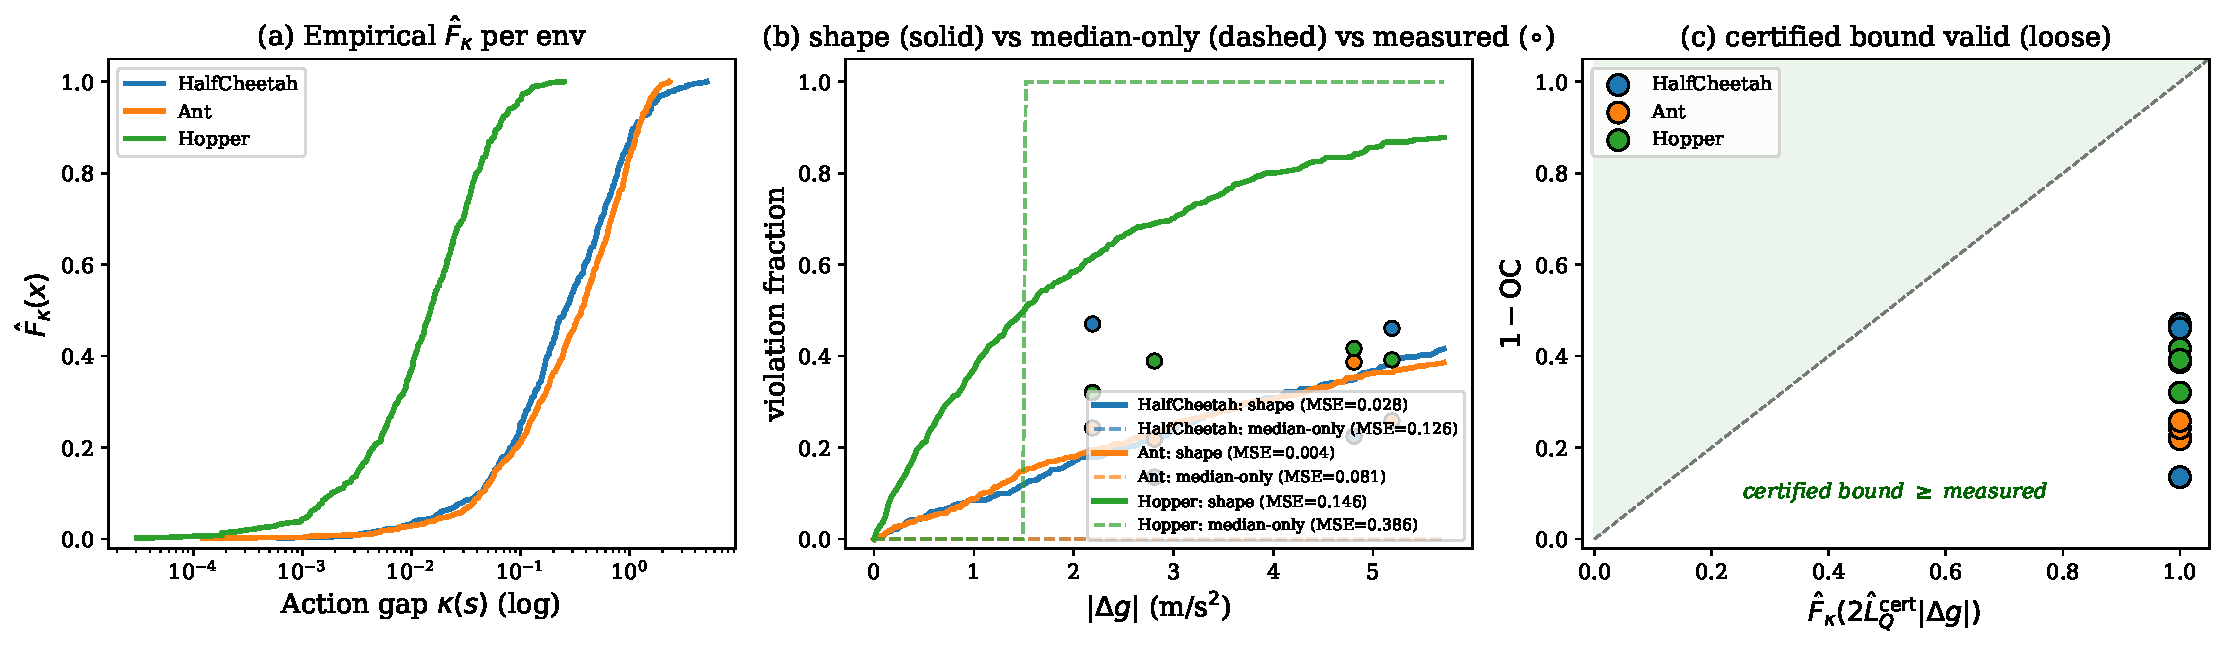
\includegraphics[width=\textwidth]{figures/exp19_fkappa_bound.pdf}
\caption{Empirical validation of Theorem~\ref{thm:violation-growth}. (a)~Empirical $\hat F_\kappa$ per environment. (b)~Head-to-head between the full-CDF predictor $\hat F_\kappa(c^* \cdot |\Delta g|)$ (solid) and a median-only predictor $\mathbf{1}[c\,|\Delta g| \geq \tilde\kappa]$ (dashed), each fit per environment by a single scalar $c$ on the measured violations ($\circ$). The shape predictor tracks the data; the median predictor degenerates to a step (zero violations until threshold, then $1$) and misses the gradual ramp on every environment. (c)~The certified bound $\hat F_\kappa(2\hat L_Q^{\mathrm{cert}} \cdot |\Delta g|)$ holds for every test (points lie inside the green region), though it saturates at $1.0$ because $\hat L_Q^{\mathrm{cert}}$ is $\sim 10^4\times$ larger than the operationally effective $c^*/2$.}
\label{fig:fkappa-bound}
\end{figure}

\begin{table}[h]
\centering
\caption{Shape vs.\ median-only predictor (mean-squared error on the 4 measured violations per env). The shape predictor strictly beats the median-only predictor on every environment by a factor of $2.6\times$--$22\times$, quantifying the population-level content the median cannot capture.}
\label{tab:shape-vs-median}
\small
\begin{tabular}{lccc}
\toprule
Env & MSE shape $\hat F_\kappa(c^* \cdot |\Delta g|)$ & MSE median-only & ratio \\
\midrule
HalfCheetah & $0.028$ & $0.126$ & $4.5\times$ \\
Ant         & $0.004$ & $0.081$ & $22.2\times$ \\
Hopper      & $0.146$ & $0.386$ & $2.6\times$ \\
\bottomrule
\end{tabular}
\end{table}

The three takeaways: (i) the theoretical bound is never violated, consistent with Theorem~\ref{thm:violation-growth}; (ii) the \emph{shape} of $\hat F_\kappa$, fit by a single environment-specific constant $c^*$, reproduces the observed violation curve in all three environments, while the best-fit median-only predictor cannot, because the violation fraction grows gradually rather than as a step (Table~\ref{tab:shape-vs-median}); and (iii) the certified Lipschitz envelope is expectedly loose ($\sim 10^4\times$ conservative), reflecting that the worst-case Q-gradient is rarely realized in on-policy states; tighter per-state Lipschitz estimation is the natural follow-up but does not affect bound validity.

\paragraph{What the certificate is for.} Because $\hat L_Q^{\mathrm{cert}}$ is $\sim 10^4\times$ larger than the operationally effective $c^*/2$, the certified bound saturates at $1.0$ on every continuous-control test in Table~\ref{tab:fkappa-bound}, and would not, on its own, gate a real deployment. We therefore frame the source-side certificate as a \emph{structural diagnostic}, not a deployment gate: it formalizes the mechanism (the violation growth depends only on $F_\kappa$ and a Lipschitz constant), it provides a comparative ranking across environments via $c^*$ that matches the empirical OC ordering ($\mathrm{Hopper} < \mathrm{Ant} < \mathrm{HalfCheetah}$), and it identifies the worst-case Lipschitz envelope as the one quantity that, if tightened by per-state estimation or domain knowledge, would close the gap between the certificate and the regime where decisions are actually made. The shape predictor in column (ii), which we view as the empirical content of Theorem~\ref{thm:violation-growth}, already produces non-trivial quantitative tracking; the worst-case envelope in column (iii) is intentionally pessimistic and is reported for completeness rather than as a usable deployment threshold.

\section{Experimental Details}
\label{app:exp-details}

\textbf{Exp 1} (Transfer Gap): $5\times5$ grid, 4 actions, $\gamma=0.95$, $\theta \in [0,1]$ (wind + cost), 50 targets.
\textbf{Exp 2} (Stability): 8-state chain, 3 actions, $\theta \in [-1,1]$ (slip + reward).
\textbf{Exp 3} (LQR): 2D mass-spring-damper, $A \in \R^{4\times4}$, $B \in \R^{4\times2}$, $Q=I$, $R=0.1I$, $\gamma=0.99$.
\textbf{Exp 4} (Control): Wind Grid $6\times6$, 4 actions; Pendulum: analytical LQR.
\textbf{Exp 5} (Sample): 6-state 3-action disagreement MDP, $\theta \sim U(-0.3, 0.7)$.
\textbf{Exp 6} (Baselines): $10\times10$ grid, $\theta \in \R^3$, $K=30$ sources, scales in $[1/r, r]$.
\textbf{Exp 7} (High-dim): 4-joint robot, 8D state, 4D action, $\theta \in \R^3$.
\textbf{Exp 8} (Neural Policy Transfer): \textbf{8a}~4-action CartPole with DQN (2-layer MLP, 64 hidden, 6 gravities, best of 2 seeds). \textbf{8b}~Standard Gymnasium: \texttt{CartPole-v1} (11 gravities, DQN best of 3 seeds, 350 episodes) and \texttt{Pendulum-v1} (LQR analytical + gym simulation, 20 gravities); Gymnasium~1.2. \textbf{8c}~MuJoCo: HalfCheetah-v4 (17D/6D), Ant-v4 (27D/8D), Hopper-v4 (11D/3D). SAC via Stable-Baselines3 (lr=$3\!\times\!10^{-4}$, batch 256, buffer 300K, 500K timesteps). Five gravities $g \in \{5.0, 7.0, 9.81, 12.0, 15.0\}$\,m/s$^2$ plus one DR agent per environment (gravity uniform in $[5.0, 15.0]$). 300 test states, seed 42.

\textbf{Exp 9} (Multi-Dim Transfer): HalfCheetah-v4 with SAC, $d=3$ parameters: gravity ($5$--$14$\,m/s$^2$), friction scale ($0.4$--$1.8$), mass scale ($0.5$--$2.0$). One source (default parameters) and 4 targets at increasing normalized $\|\Delta\thetavec\|$. Each axis normalized by half-range (gravity$/5.0$, friction$/0.85$, mass$/0.75$). Same SAC hyperparameters as Exp~8c. 300 test states, 20 eval episodes, seed 42.

All experiments use deterministic seeds for reproducibility: Exp 1--7 use \texttt{numpy} seed $42$ (and where applicable a derived seed $42{+}100$ for the second sampling pass in Exp 6 and Exp 3); Exp 8a--8b use the seed lists already noted above; Exp 8c--9 use \texttt{numpy} seed $42$ at the driver level and pass the same seed to Stable-Baselines3 / Gymnasium environments (with the multi-seed extension running over $\{42, 123, 7\}$ where reported). Code is provided in the supplementary material. Total runtime: $\sim$20 minutes on a single CPU for Exp 1--7; Exp 8a--8b use PyTorch on CPU; Exp 8c--9 require $\sim$14 hours on GPU (NVIDIA RTX 4070 SUPER) for SAC training.

% ────────────────────────────────────────────────────────────
\section{Multi-Dimensional Parameter Transfer (\texorpdfstring{$d = 3$}{d = 3})}
\label{app:exp-multidim}
% ────────────────────────────────────────────────────────────

Experiments 1--8 vary a single parameter (gravity). Real sim-to-real gaps involve simultaneous shifts in multiple physics parameters. This experiment tests whether ordinal transfer extends to $\thetavec \in \R^d$ with $d = 3$: gravity ($5$--$14$\,m/s$^2$), friction scale ($0.4$--$1.8$), and mass scale ($0.5$--$2.0$), all varying simultaneously on HalfCheetah-v4 with SAC.

We train one source agent at default parameters ($g = 9.81$, friction $= 1.0$, mass $= 1.0$) and 4 target agents at increasing normalized distances $\|\Delta\thetavec\|$: small ($\|\Delta\thetavec\| \approx 0.24$), medium ($\approx 0.57$), large ($\approx 1.17$), and extreme ($\approx 1.60$).

Table~\ref{tab:multidim} and Figure~\ref{fig:multidim} summarize the results:

\begin{table}[h]
\centering
\caption{Multi-dimensional transfer results ($d=3$, HalfCheetah-v4). Source return = source policy deployed at target; Target return = policy trained at target.}
\label{tab:multidim}
\begin{tabular}{lccccc}
\toprule
Target & $\|\Delta\thetavec\|$ & Source Return & Target Return & Directional OC & Action Disp. \\
\midrule
small-1   & 0.241 & 10{,}451 & 10{,}429 & 0.831 & 1.033 \\
med-1     & 0.573 &  9{,}420 &  9{,}091 & 0.672 & 1.865 \\
large-1   & 1.171 &  7{,}265 &  7{,}840 & 0.662 & 2.096 \\
extreme-1 & 1.600 &  5{,}905 &  5{,}374 & 0.467 & 2.758 \\
\bottomrule
\end{tabular}
\end{table}

\emph{Transfer robustness}: the source policy achieves return comparable to or exceeding the target-trained policy at 3 of 4 shift magnitudes (small-1, med-1, extreme-1); at large-1 ($\|\Delta\thetavec\| = 1.17$) the target-trained policy is better by $575$ return units (Figure~\ref{fig:multidim}(a)). Notably at extreme shifts ($\|\Delta\thetavec\| = 1.60$), the source policy scores $5{,}905$ vs.\ the target-trained $5{,}374$, suggesting that 500K training steps are insufficient for the target-trained agent to converge in the extreme regime, while the source policy's learned behavior remains competitive.

\emph{OC decay}: directional OC decreases monotonically with $\|\Delta\thetavec\|$, from $0.83$ at small shifts to $0.47$ at extreme shifts, mirroring the 1D gravity-only trend from Exp~8c.

\emph{Scale-invariance}: majority vote maintains perfect agreement ($= 1.000$) across all multi-dimensional shifts and rescaling levels up to $100\times$, while mean-action degrades to $0.80$, confirming that scale-invariance holds for $d > 1$.

\emph{Action displacement}: mean displacement grows linearly with $\|\Delta\thetavec\|$ ($1.03 \to 2.76$, slope $\approx 1.12$), consistent with Theorem~\ref{thm:action-displacement} (Appendix~\ref{app:proofs}).

\emph{Key finding}: the ordinal framework's predictions extend naturally from $d=1$ to $d=3$: OC decay, scale-invariance, and action displacement all depend on $\|\Delta\thetavec\|$ regardless of which combination of physics parameters varies.

\begin{figure}[h]
\centering
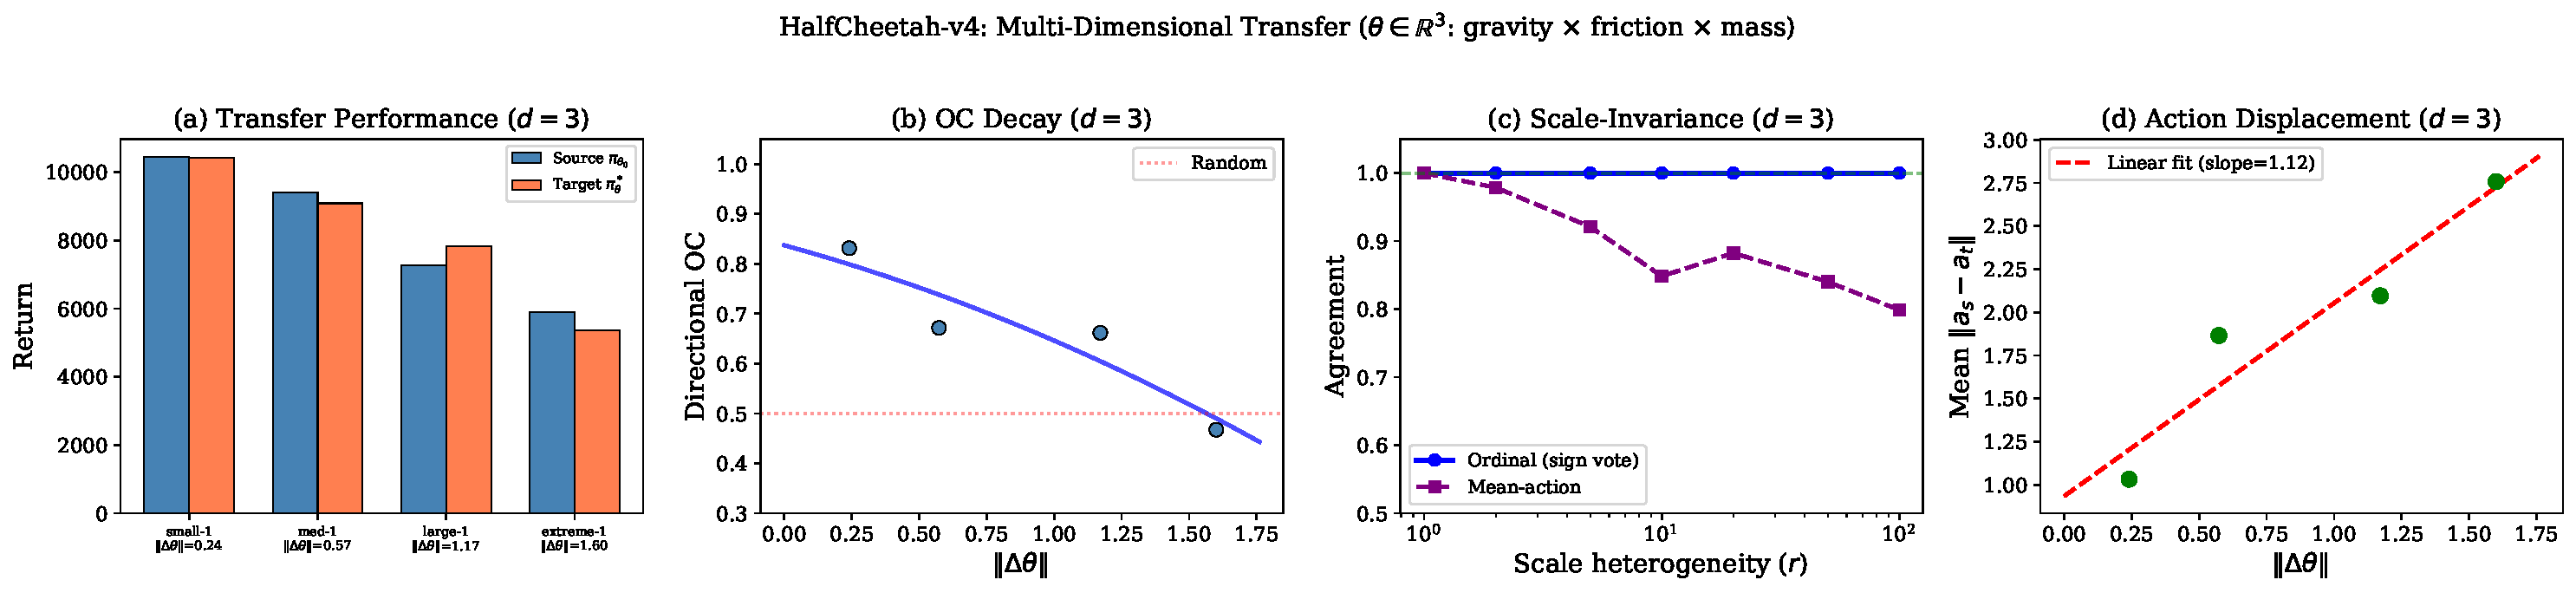
\includegraphics[width=\textwidth]{figures/exp11_multidim_transfer.pdf}
\caption{Multi-dimensional transfer ($d=3$): HalfCheetah with SAC, varying gravity $\times$ friction $\times$ mass simultaneously. (a) Source policy (blue) vs.\ target-trained (orange): source remains competitive even at extreme shifts. (b) Directional OC decay. (c) Scale-invariance: MV $=1.000$; MA degrades. (d) Action displacement grows linearly (slope $\approx 1.12$).}
\label{fig:multidim}
\end{figure}

% ────────────────────────────────────────────────────────────
\section{Tightness of \texorpdfstring{$F_\kappa$}{F\_kappa} Bound across Discount Factors}
\label{app:gamma-tightness}
% ────────────────────────────────────────────────────────────

Propositions~\ref{prop:tight-growth} and~\ref{prop:tight-growth-gamma} establish that the violation growth bound $F_\kappa(2L_Q\|\Delta\theta\|)$ is tight to factor $1$ for every $\gamma \in [0, 1)$ on a saturating MDP family (a self-loop construction at $\gamma = 0$; an action-dependent transition construction for $\gamma > 0$). We now test the bound on a different (non-worst-case) family to see how much slack appears when the actual Q-Lipschitz constant of the tested MDP lies below the worst-case envelope.

\paragraph{Setup.} 20-state chain MDP with 3 actions and linearly spaced action gaps $\kappa(s) \in [0.05, 1.0]$. The parameter $\theta$ shifts rewards to flip action orderings progressively (small-gap states first). Transitions are $\theta$-independent, isolating the effect of $\gamma$ on Q-value propagation through reward changes alone. \emph{Caveat}: because transitions are $\theta$-independent, the cascade effect described in Remark~4 (where one state's ordering flip propagates through the value function to cause secondary flips) is limited. With state-dependent transitions, the bound could degrade further; testing this remains future work.

\paragraph{Results.} Figure~\ref{fig:gamma-tight} shows the $F_\kappa$ bound (red step function) vs.\ actual violation fraction (blue dots) across five discount factors.

\begin{table}[h]
\centering
\caption{Tightness ratio (bound/actual) of the violation growth bound $F_\kappa(2L_Q\|\Delta\theta\|)$ across discount factors. At $\gamma=0$ the bound is exactly tight; tightness degrades gracefully with $\gamma$.}
\label{tab:gamma-tight}
\begin{tabular}{ccccc}
\toprule
$\gamma$ & $L_Q$ & Avg Ratio & Max Actual & Max Bound \\
\midrule
0.00 &  1.0 & 1.0$\times$ & 1.000 & 1.000 \\
0.50 &  2.0 & 1.4$\times$ & 1.000 & 1.000 \\
0.90 & 10.0 & 2.0$\times$ & 0.900 & 1.000 \\
0.95 & 19.9 & 2.7$\times$ & 0.700 & 1.000 \\
0.99 & 93.4 & 5.2$\times$ & 0.900 & 1.000 \\
\bottomrule
\end{tabular}
\end{table}

The bound is exactly tight at $\gamma = 0$ (ratio $= 1.0\times$), remains within a factor of 2 at $\gamma = 0.9$, and reaches $5.2\times$ at $\gamma = 0.99$. The looseness at high $\gamma$ is consistent with Proposition~\ref{prop:tight-growth-gamma}: the chain MDP's actual Q-Lipschitz constant lies below the worst-case $L_R/(1-\gamma)$ used in the bound's argument, so plugging in the worst-case value overestimates flips for this specific (non-self-loop) family. On the self-loop construction of Proposition~\ref{prop:tight-growth-gamma}, the same bound would be exactly saturated at every $\gamma$. The bound is therefore a valid upper bound at all $\gamma$, and tighter MDP-specific estimates of $L_Q$ recover the gap.

\begin{figure}[h]
\centering
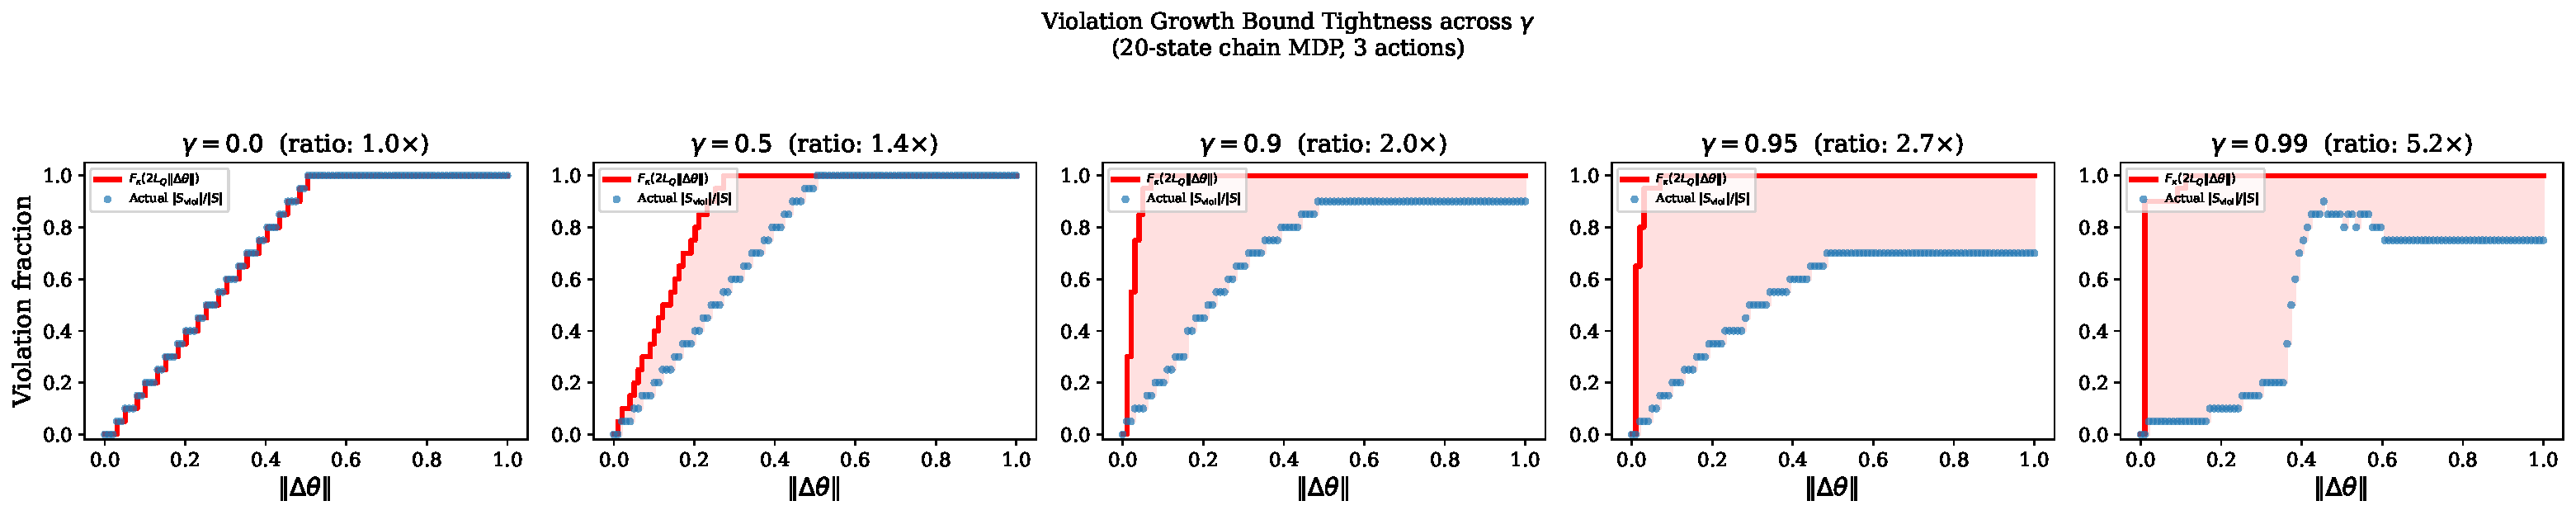
\includegraphics[width=\textwidth]{figures/exp12_gamma_tightness.pdf}
\caption{Tightness of the $F_\kappa$ violation growth bound across discount factors. Red: predicted bound $F_\kappa(2L_Q\|\Delta\theta\|)$. Blue dots: actual $|S_{\mathrm{viol}}|/|S|$. Pink shading: gap between bound and actual. The bound is exact at $\gamma=0$ and degrades gracefully.}
\label{fig:gamma-tight}
\end{figure}

% ────────────────────────────────────────────────────────────
\section{Per-State Violation Order}
\label{app:perstate}
% ────────────────────────────────────────────────────────────

Theorem~\ref{thm:violation-growth} predicts that states violate \emph{in order of increasing action gap} $\kappa(s)$: states with small gaps are the first to flip their optimal action as $\|\Delta\theta\|$ increases. We verify this prediction directly.

\paragraph{Setup.} For three tabular MDPs (5$\times$5 grid, 20-state chain, 6$\times$6 cliff), we compute the action gap $\kappa(s)$ at the source and sweep $\theta$ to find, for each state $s$, the smallest $\|\Delta\theta\|$ at which $\pi^*_{\theta_0}(s) \neq \pi^*_\theta(s)$ (the ``violation threshold'').

\paragraph{Results.} Figure~\ref{fig:perstate} plots action gap vs.\ violation threshold for each state. The positive correlation is clear: small-gap states (bottom-left) violate at small $\|\Delta\theta\|$, while large-gap states (top-right) resist perturbation or never violate. On the 20-state chain (where action gaps are linearly spaced by construction), the Pearson correlation is $r = 0.56$ ($R^2 = 0.31$) among the 14 states that violate, and 6 states with the largest gaps never violate within $\|\Delta\theta\| \leq 1.0$. This is exactly the mechanism underlying Theorem~\ref{thm:violation-growth}: $F_\kappa(2L_Q\|\Delta\theta\|)$ counts the fraction of states whose gap is below a threshold, and those are precisely the states that have already flipped.

\begin{figure}[h]
\centering
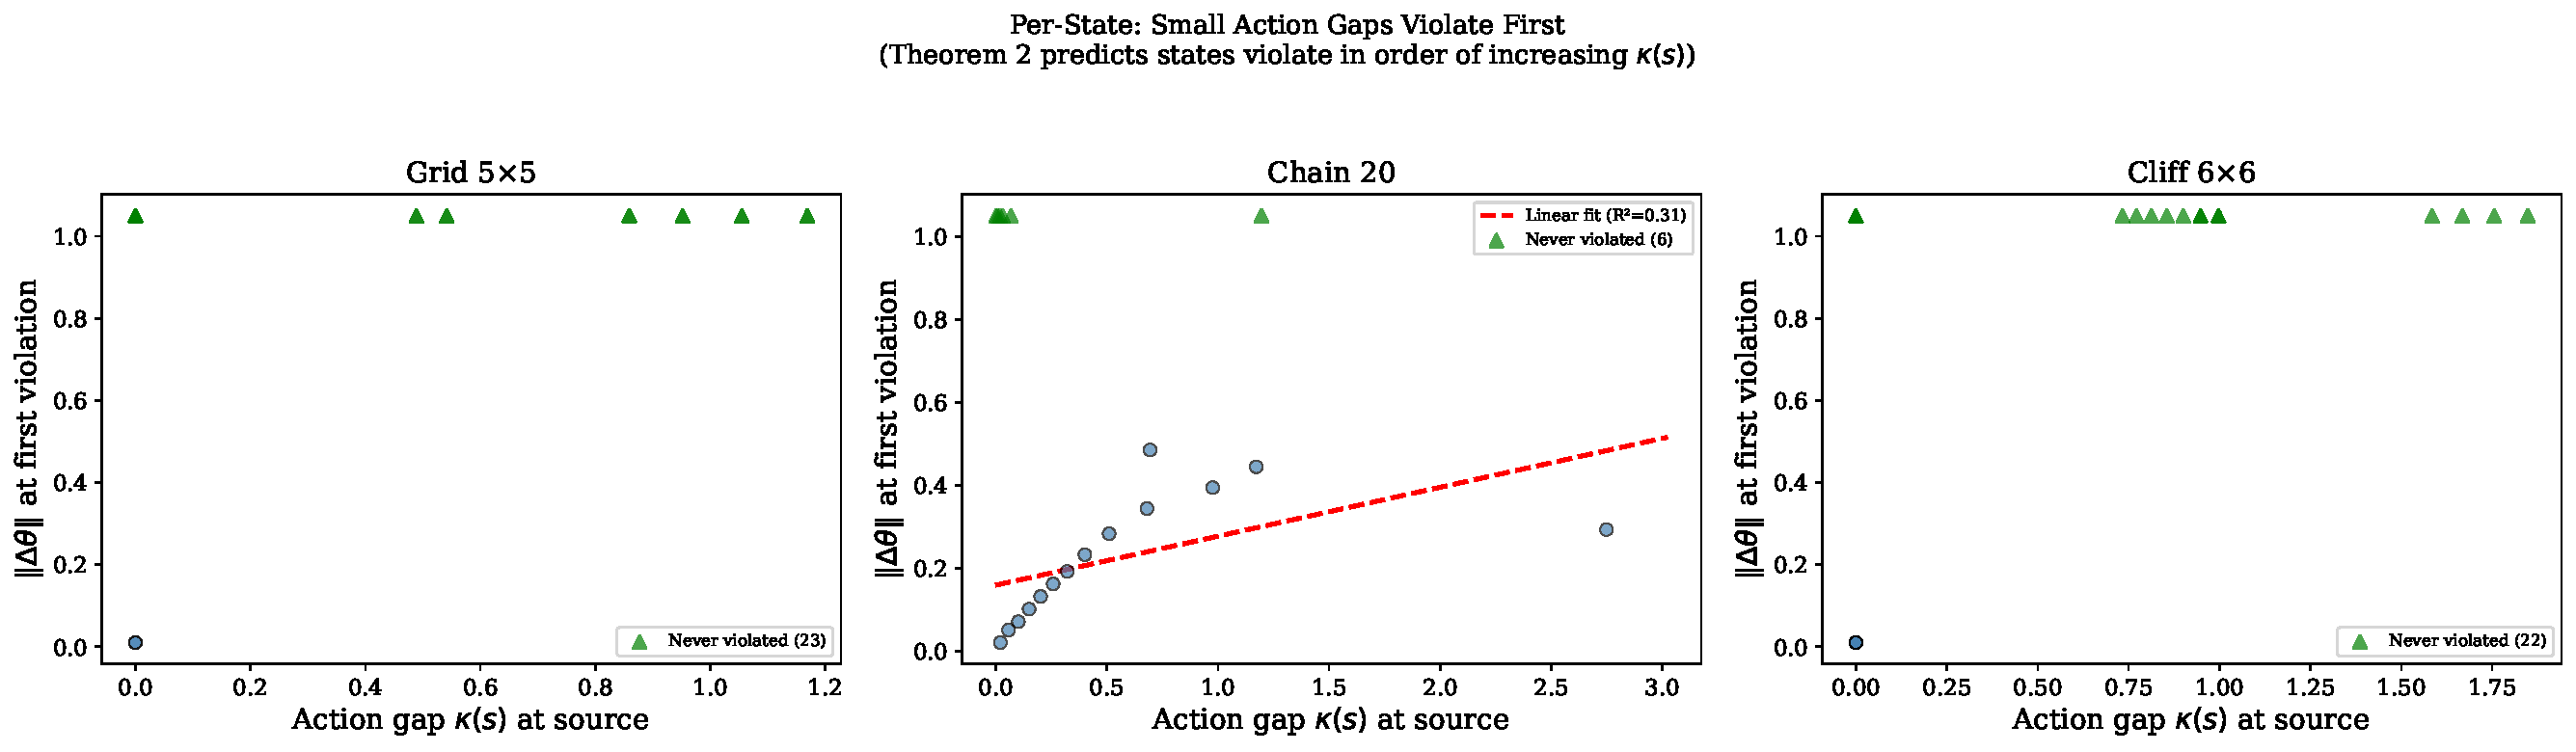
\includegraphics[width=\textwidth]{figures/exp13_perstate_violation.pdf}
\caption{Per-state violation order. Each dot is a state $s$; $x$-axis is the action gap $\kappa(s)$ at the source, $y$-axis is the smallest $\|\Delta\theta\|$ at which the state's optimal action changes. Green triangles: states that never violate within $\|\Delta\theta\| \leq 1.0$. Small-gap states violate first, confirming the mechanism behind Theorem~\ref{thm:violation-growth}.}
\label{fig:perstate}
\end{figure}

% ────────────────────────────────────────────────────────────
\section{Hessian Diagnostic for Strong Concavity}
\label{app:hessian-diag}
% ────────────────────────────────────────────────────────────

Cross-seed-mean log-log slopes (Table~\ref{tab:slope-comparison}) place HalfCheetah ($1.20$) and Hopper ($1.17$) below the quadratic upper bound of Theorem~\ref{thm:continuous-bound-main} and Ant ($2.52$) above it, the latter driven by light-gravity cells (Section~\ref{sec:exp-mujoco-transfer}). Single-seed-42 fits used in Figure~\ref{fig:mujoco-transfer} are larger ($4.56/4.19/1.88$) and reflect single-cell sample noise; this appendix provides direct empirical evidence that the same environments, gravities, and direction where the slope is largest are also where Assumption~\ref{asm:local-sc} measurably fails.

\paragraph{Setup.} For each environment and each gravity $g \in \{5.0, 7.0, 9.81, 12.0, 15.0\}$, we load the SAC model trained at that gravity and collect $150$ on-policy states via rollouts at the same gravity. At each state $s$, we (i) refine the SAC action $a$ via $80$ gradient-ascent steps on the critic $Q_1(s, \cdot)$ starting from the policy output, producing a local Q-maximizer $a^\star(s)$, and (ii) estimate the action-Hessian $\nabla^2_{aa} Q_1(s, a^\star(s))$ via symmetric finite differences along $\geq 4 d_a(d_a+1)/2$ random unit directions ($\varepsilon = 0.05$ of the action range), recovering the $d_a \times d_a$ matrix via least-squares. We then compute the \emph{strong-concavity margin} $\mu(s) := -\lambda_{\max}(\nabla^2_{aa} Q_1(s, a^\star(s)))$, which is bounded below by $\mu > 0$ under Assumption~\ref{asm:local-sc}.

Finite differences are required because SAC's critic is a ReLU MLP: it is piecewise linear, so analytic Hessians vanish almost everywhere. Finite differences at scale $\varepsilon$ capture the \emph{effective} curvature over a neighborhood spanning multiple linear pieces, which is the quantity the strong concavity assumption is about at a non-asymptotic scale.

\paragraph{Results.} Figure~\ref{fig:hessian} shows the median of $\mu(s)$ and its interquartile range across states, per environment. Two quantitative observations:

\emph{Collapse of concavity at shifted gravities.} For HalfCheetah, the source-gravity margin (median $\mu = 8.93$) drops by 5--15$\times$ at all shifted gravities (median $\mu \in [0.60, 2.11]$), confirming that the strong concavity bound is not preserved under parameter shift. For Ant, the margin actually becomes \emph{negative} at $g=5$ (median $\mu = -0.90$; $53\%$ of states have non-concave $Q$ at their policy output), coinciding with the multi-seed experiment's most severe source-policy failure on Ant ($g=5$: $143 \pm 72$ vs.\ target $1{,}723 \pm 404$, Table~\ref{tab:multiseed}).

\emph{Near-quadratic environment has uniform but shallow curvature.} Hopper's margin is smaller in absolute scale ($\mu \in [0.15, 1.64]$) and relatively flat across gravities. This is consistent with its near-quadratic transfer-gap slope (cross-seed-mean ${\approx}1.17$, single-seed-42 ${\approx}1.88$): when concavity is weak but \emph{uniform}, the smooth-deformation argument of Theorem~\ref{thm:quadratic-subopt} still applies. The sharp, localized $\mu$ collapse seen on HalfCheetah and the sign flip on Ant inflate \emph{single-seed} slopes ($4.56$ and $4.19$) at seed $42$; under cross-seed averaging only Ant's slope ($2.52$) actually exceeds quadratic, traced to a directional precondition failure analyzed below.

\begin{figure}[h]
\centering
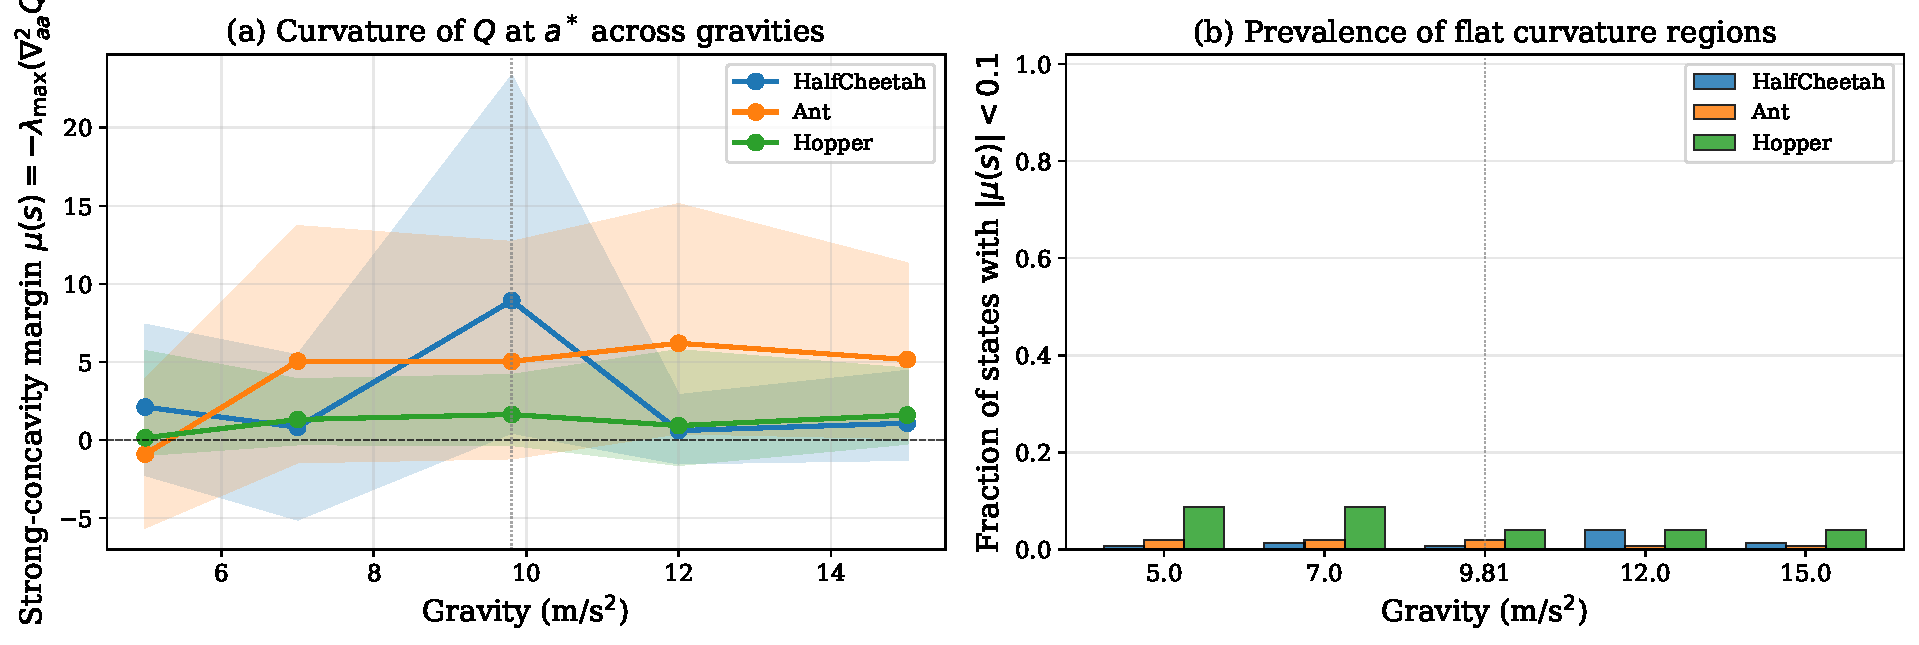
\includegraphics[width=\textwidth]{figures/exp16_hessian_diagnostic.pdf}
\caption{Strong-concavity margin $\mu(s) = -\lambda_{\max}(\nabla^2_{aa} Q)$ at the Q-maximizing action, across gravities, per environment ($150$ on-policy states each). (a) Median and interquartile range; HalfCheetah drops sharply from source $\mu \approx 9$ to $\mu \lesssim 2$ at shifted gravities, and Ant's margin becomes negative at $g=5$. Hopper is uniformly mild. (b) Fraction of states with $|\mu(s)| < 0.1$.}
\label{fig:hessian}
\end{figure}

These measurements directly corroborate the strong-concavity breakdown narrative and explain why HalfCheetah and Ant exceed the theoretical quadratic rate, while Hopper remains close to it. The diagnostic does not claim to replace a rigorous theorem for the multi-basin regime, which remains open (Assumption~\ref{asm:basin-dom}); it shows that the qualitative condition our upper bound requires is empirically violated in the same environments and at the same gravities where the bound is observed to loosen. An exploratory state-level decomposition pairing per-state Monte-Carlo gap contributions $V^{\pi^*_g}_g(s) - V^{\pi_{\rm src}}_g(s)$ with $\mu(s)$ ($60$ on-policy states per (env, gravity) cell, seed 42) finds that the non-concave subset $\{s : \mu(s) \leq 0\}$ contributes a similar share of the cell-level transfer gap on all three environments ($\approx 30$--$35\%$). This indicates that elevated \emph{pointwise} non-concavity is not what distinguishes Ant from HalfCheetah/Hopper; what differs is \emph{where} the non-concavity manifests and how directionally it is concentrated, as shown next.

\paragraph{Why Ant exceeds the bound (directional reading).} Two complementary measurements localize Ant's $\approx 2.52$ slope as a directional boundary case rather than a general framework failure.

\emph{Direction asymmetry.} Pairing target gravities at matched $|\Delta g|$ (cross-seed-mean cell-level gaps), the lighter-vs-heavier ratio $\mathrm{gap}_{\rm heavy}/\mathrm{gap}_{\rm light}$ is sharply environment-specific:
\begin{center}
\small
\begin{tabular}{lcc}
\toprule
$|\Delta g|$ & $g_{\rm light}=7,\,g_{\rm heavy}=12$ & $g_{\rm light}=5,\,g_{\rm heavy}=15$ \\
\midrule
HalfCheetah & $0.39$ & $0.85$ \\
Ant         & $\mathbf{0.06}$ & $\mathbf{0.54}$ \\
Hopper      & $1.52$ & $1.77$ \\
\bottomrule
\end{tabular}
\end{center}
Ant concentrates $16\times$ more transfer gap in the lighter direction at $|\Delta g|=2.5$; HalfCheetah is mildly asymmetric; Hopper has the opposite asymmetry (heavier is harder). The lighter direction is exactly where median $\mu(s)$ flips negative on Ant ($g{=}5$), so the slope-exceedance is driven by a one-sided precondition failure, not a uniform breakdown across the gravity range.

\emph{Per-seed slope dispersion.} Per-seed log-log slopes have std $2.4$--$3.4$ across all three environments, dominated by single $(\text{seed}, g)$ cells where the source incidentally outperforms the target (clipped at $\mathrm{gap}=1$). For Ant specifically, the per-seed slopes are $\{1.60, 6.70, 1.72\}$ on seeds $\{42, 123, 7\}$: the $> 2$ headline is driven by seed 123 alone; seeds 42 and 7 both sit below $2$, again consistent with quadratic scaling on the side where the bound's preconditions hold.

Together, these readings frame Ant as marking the boundary of Theorem~\ref{thm:continuous-bound-main}'s regime: the bound holds on the side where Assumption~\ref{asm:local-sc} is preserved (heavier gravities; majority of seeds), and breaks predictably where it is not (lighter gravities, where the policy expects body weight that is no longer present and a non-concave critic surface emerges). The two diagnostics above are complementary, not redundant: the per-state non-concavity \emph{share} is uniform across environments ($\approx 30$--$35\%$), so Ant's exceedance cannot be attributed to elevated pointwise breakdown; what is environment-specific is the directional concentration (the $0.06$ light/heavy ratio at $|\Delta g|=2.5$) coinciding with median-$\mu$ sign-flip on the same side. A multi-basin / direction-aware extension of the bound is left to future work.

% ────────────────────────────────────────────────────────────
\section{Covering-Number Extension of the Source-Agreement Certificate}
\label{app:covering-number}
% ────────────────────────────────────────────────────────────

The union bound in Proposition~\ref{prop:model-free} scales as $|\cS|\binom{|\cA|}{2}$, which is intractable for continuous or large discrete state spaces. A natural extension is to construct the certificate over a finite $\epsilon$-covering of $\cS$ (of size $\cN(\cS, \epsilon)$) and interpolate via the Lipschitz continuity of Q-gaps (Lemma~\ref{lem:q-lipschitz}), replacing $|\cS|$ with $\cN(\cS, \epsilon)$ at the cost of an additive $O(\epsilon L_Q)$ slack in the margin estimate.
The optimal $\epsilon$ balances two competing effects: the margin slack $\epsilon L_Q$ (favoring small $\epsilon$) against the sample requirement $K \gtrsim \kappa_{\min}^{-2}\ln(\cN(\cS,\epsilon)\binom{|\cA|}{2}/\delta)$ (favoring large $\epsilon$). Setting $\epsilon L_Q = \hat{\kappa}/2$ (half the estimated margin) and solving yields $\epsilon^* = \hat{\kappa}/(2L_Q)$, which equals the stability radius itself---an intuitive result: the covering resolution need not be finer than the transfer region being certified.
For state spaces with polynomial covering numbers $\cN(\cS, \epsilon) = O(\epsilon^{-d_s})$, this gives
\[
K = O\!\left(\kappa_{\min}^{-2}\bigl(d_s\ln(L_Q/\kappa_{\min}) + \ln(|\cA|/\delta)\bigr)\right),
\]
scaling logarithmically in the effective state-space dimension $d_s$. This covering-number approach integrates naturally with function approximation settings where states are represented in a continuous feature space.

\end{document}
